\documentclass[12pt]{article}

% Packages
\usepackage[utf8]{inputenc}
\usepackage[margin=1in]{geometry}
\usepackage{amsmath,amssymb,amsthm}
\usepackage{graphicx}
\usepackage{booktabs}
\usepackage{longtable}
\usepackage{setspace}
\usepackage{natbib}
\usepackage{hyperref}
\usepackage{caption}
\usepackage{subcaption}
\usepackage{float}
\usepackage{threeparttable}
\usepackage{multirow}
\usepackage{pdflscape}
\usepackage{xcolor}

% Graphics path for figures
\graphicspath{{Data/output/figures_methods/}}

% Hyperref setup
\hypersetup{
    colorlinks=true,
    linkcolor=blue!70!black,
    citecolor=blue!70!black,
    urlcolor=blue!70!black
}

% Double spacing
\doublespacing

% Theorem environments
\newtheorem{proposition}{Proposition}
\newtheorem{remark}{Remark}

% Title
\title{When $K$ Matters: Model Selection in Finite Mixtures\\ and the Magnitude of Policy Counterfactuals}

\author{Alina Malkova\thanks{Department of Economics, Nathan M.\ Bisk College of Business, Florida Institute of Technology. Email: \href{mailto:amalkova@fit.edu}{amalkova@fit.edu}. I thank [names] for helpful comments. All errors are my own.}}

\date{March 2026}

\begin{document}

\maketitle

\begin{abstract}
\noindent The number of mixture components $K$ in finite mixture models---typically treated as a technical detail---can be the dominant source of uncertainty in counterfactual policy analysis. I develop a three-pronged selection framework combining information criteria, counterfactual stability, and penalized estimation. In an application to bank branch access and self-employment, counterfactual predictions range from $-0.6\%$ ($K=1$) to $-10.8\%$ ($K=4$)---an 18-fold difference that dwarfs all other specification uncertainty by an order of magnitude. Monte Carlo simulations show this arises from a \textit{cancellation condition}: when type-specific effects have opposite signs, the true $K$ is recovered in fewer than 10\% of replications. Rather than selecting a single $K$, I report bounds under model uncertainty and a Bayesian Dirichlet process posterior that integrates over $K$, yielding $-8.5\%$ (95\% CI: $[-14.2\%, -3.1\%]$).

\vspace{0.5cm}
\noindent \textbf{JEL Codes:} C25, C38, C52, C11

\vspace{0.3cm}
\noindent \textbf{Keywords:} Finite mixture models, model selection, number of components, counterfactual analysis, unobserved heterogeneity, policy evaluation
\end{abstract}

\newpage

%%%%%%%%%%%%%%%%%%%%%%%%%%%%%%%%%%%%%%%%%%%%%%%%%%%%%%%%%%%%%%%%%%%%%%%%%%%%%%%
\section{Introduction}
%%%%%%%%%%%%%%%%%%%%%%%%%%%%%%%%%%%%%%%%%%%%%%%%%%%%%%%%%%%%%%%%%%%%%%%%%%%%%%%

Finite mixture models have become a workhorse tool in applied economics. Researchers use them to capture unobserved heterogeneity in treatment responses \citep{heckman1984}, consumer preferences \citep{keane1997}, dynamic discrete choices \citep{arcidiacono2011}, labor market sorting \citep{bonhomme2019}, and firm behavior \citep{fox2011}. The practical challenge of selecting the number of mixture components $K$---too few types mask economically meaningful heterogeneity; too many invite overfitting and unstable estimates---is well understood in econometric theory \citep{kasahara2009, compiani2016, chen2001}. Yet in applied practice, $K$ selection is typically relegated to a footnote: researchers report a BIC-preferred specification and conduct at most cursory sensitivity analysis.

This paper demonstrates that this practice can be dangerously misleading. In the application I study, assumptions about $K$ swing counterfactual policy predictions by a factor of eighteen---dwarfing all other sources of specification uncertainty combined. The methodological insight is simple but underappreciated: when type-specific treatment effects have opposite signs, the aggregate counterfactual is a weighted average that depends critically on whether the analyst permits enough types to separate the underlying heterogeneity.

I develop and demonstrate a general framework for $K$ selection in finite mixture counterfactual analysis, illustrated using the relationship between bank branch access and self-employment. A companion paper \citep{malkova2026substantive} documents a robust reduced-form null for this application, providing a sharp benchmark for the structural analysis.

Monte Carlo simulations with two complementary designs reveal the severity of the problem. The ``cancellation'' design---where type-specific effects have opposite signs, producing a near-zero aggregate---generates within-replication counterfactual ranges of 15--17~pp across $K$, mirroring the empirical finding. Crucially, the true $K=4$ is recovered in fewer than 10\% of replications even at $N = 50{,}000$, because the cancellation mechanism makes types statistically near-indistinguishable. Under the ``same-sign'' control design, counterfactual magnitudes still vary with $K$ but the qualitative conclusion is robust. These findings motivate the bounds and Bayesian model averaging approach developed below.

In the empirical application, a multinomial logit with $K=4$ latent types identifies four economically distinct population segments, and the counterfactual jumps from $-0.6\%$ ($K=1$) to $-10.8\%$ ($K=4$). The 18-fold difference arises because the homogeneous model averages opposite-signed type-specific effects, producing a near-zero aggregate that obscures substantial within-type heterogeneity.

To discipline $K$ selection, I develop a three-pronged approach combining three recent advances: (i) Hao and Kasahara (2025) panel BIC, which adjusts the penalty for repeated cross-sections of the same markets; (ii) Bonhomme, Lamadon, and Manresa (2022) counterfactual stability, which selects the smallest $K$ at which the policy prediction stabilizes; and (iii) Budanova (2025) penalized MLE, approximated via overspecification and significance-based classification of active types. All three methods select $K=4$. However, the counterfactual sensitivity analysis demonstrates that even well-motivated selection methods leave substantial residual model uncertainty.

Rather than reporting a single $K$-selected point estimate, I present three complementary summaries of the counterfactual:
\begin{enumerate}
    \item \textit{Bounds under model uncertainty}: $\Delta SE \in [-10.8\%, -0.6\%]$, valid for any $K \in \{1, \ldots, 5\}$.
    \item \textit{Bayesian posterior integrating over $K$}: mean $-8.5\%$, 95\% credible interval $[-14.2\%, -3.1\%]$, $P(\text{effect} < 0) = 0.99$.
    \item \textit{BIC-selected point estimate}: $-10.8\%$ under $K=4$.
\end{enumerate}

The discrepancy between the structural findings and the reduced-form null creates a genuine interpretive tension. The structural interpretation is that the reduced-form null reflects cancellation across types, not absence of effects. The skeptical interpretation is that the structural heterogeneity is an artifact of functional form---the mixture model discovers types that happen to separate demographic groups with different self-employment rates, with no causal credit channel. I do not resolve this tension; doing so requires exogenous variation in branch access that the data do not provide. Instead, I develop a framework for transparently reporting results under both views, demonstrating how bounds and Bayesian model averaging can accommodate irreducible model uncertainty.

\subsection{Contributions}

The primary contribution is demonstrating that $K$ selection in finite mixture models can be the dominant source of uncertainty in counterfactual policy analysis. Table~\ref{tab:uncertainty_decomp} (previewed here, presented in Section~\ref{sec:uncertainty}) decomposes the sources of specification uncertainty in the counterfactual: $K$ selection generates a $19\times$ range, while statistical sampling uncertainty ($1.9$--$3.2\times$), discrete vs.\ continuous heterogeneity ($1.1\times$), and reduced-form control specification ($1.2\times$) are all an order of magnitude smaller. This finding implies that any applied paper using finite mixtures should report sensitivity to $K$ alongside standard robustness checks.

The paper contributes to several literatures:

\textit{Finite mixture model selection.} I extend the work of \citet{kasahara2009}, \citet{compiani2016}, \citet{hao2025}, \citet{budanova2025}, and \citet{bonhomme2022} by showing that even when multiple selection criteria agree on $K$, the counterfactual implications can differ sharply from reduced-form evidence. The three-pronged framework integrates complementary selection perspectives and makes residual model uncertainty transparent.

\textit{Structural vs.\ reduced-form methods.} The tension between structural and reduced-form identification is a central methodological debate in economics \citep{heckman2010, angrist2010, keane2010, nevo2010}. I demonstrate a concrete setting where the two approaches yield qualitatively different policy conclusions and develop a framework for reporting results under both views.

\textit{Sensitivity analysis and model uncertainty.} The paper connects to the growing literature on reporting model uncertainty in applied work \citep{leamer1983, oster2019, cinelli2020, andrews2023}, extending these tools to the mixture model context. The bounds-based approach I develop parallels partial identification methods \citep{manski2003} but operates over the model space rather than the parameter space.

\textit{Monte Carlo evidence on $K$ selection.} The Monte Carlo simulations contribute to the finite sample understanding of mixture model selection criteria. The two-design comparison identifies a simple sufficient condition---opposite-signed type effects---under which $K$ selection dominates all other specification choices.

The paper proceeds as follows. Section~\ref{sec:lit} reviews the literature on $K$ selection. Section~\ref{sec:framework} presents the model selection framework. Section~\ref{sec:montecarlo} examines $K$ recovery and counterfactual sensitivity via Monte Carlo simulation. Section~\ref{sec:application} describes the empirical application. Section~\ref{sec:results} presents the main results. Section~\ref{sec:tension} discusses the reduced-form/structural tension. Section~\ref{sec:uncertainty} quantifies the sources of specification uncertainty. Section~\ref{sec:conclusion} concludes with recommendations for applied practice.


%%%%%%%%%%%%%%%%%%%%%%%%%%%%%%%%%%%%%%%%%%%%%%%%%%%%%%%%%%%%%%%%%%%%%%%%%%%%%%%
\section{Related Literature on $K$ Selection}
\label{sec:lit}
%%%%%%%%%%%%%%%%%%%%%%%%%%%%%%%%%%%%%%%%%%%%%%%%%%%%%%%%%%%%%%%%%%%%%%%%%%%%%%%

\subsection{Theoretical Foundations}

Testing the number of components in mixture models is complicated by nonstandard asymptotics: under $H_0: K = K_0$, the likelihood ratio statistic does not have a $\chi^2$ distribution because parameters of the additional component lie on the boundary of the parameter space \citep{chen2001, chen2009}. \citet{kasahara2009} develop a modified likelihood ratio test for panel data that exploits the additional information from repeated observations, showing that repeated measurements restore standard asymptotics for the LR test. \citet{kasahara2014} extend this to dynamic models with state dependence.

Information criteria offer a practical alternative. The standard BIC \citep{schwarz1978} penalizes model complexity by $p \cdot \ln(N)$, where $p$ is the number of free parameters and $N$ the sample size. \citet{compiani2016} provide a comprehensive treatment for economic applications, showing that BIC performs well in simulations but can be sensitive to sample size and parameter dimensionality. \citet{hao2025} develop a panel-specific BIC that replaces $N$ with $N_{panels}$ and adds a correction factor $c(T) = 1 + 1/T$ for the number of time periods:
\begin{equation}
\text{Panel BIC}(K) = -2\ln\mathcal{L}(K) + p_K \cdot \ln(N_{panels}) \cdot c(T)
\label{eq:panelbic}
\end{equation}
This adjustment addresses the tendency of standard BIC to over-select when applied to panel data, where the effective number of independent units is smaller than $N$.

\subsection{Penalized and Bayesian Approaches}

An alternative to information criteria is penalized likelihood, which shrinks redundant component shares toward zero. \citet{budanova2025} proposes penalized MLE for mixture models where the penalty term encourages sparsity in the mixing weights $\pi_k$. Under appropriate regularity conditions, the estimator consistently selects $K$ while maintaining parametric convergence rates for the identified parameters.

Bayesian nonparametric methods avoid selecting $K$ altogether by placing a prior over the space of mixing distributions. The Dirichlet Process Mixture (DPM) model \citep{ferguson1973, antoniak1974} uses a Dirichlet process prior on the mixing distribution, allowing the effective number of components to be determined by the data. \citet{malsiner2016} develop sparse finite mixture models that place a symmetric Dirichlet prior $\text{Dir}(e_0, \ldots, e_0)$ on mixing weights with $e_0 < 1$, encouraging sparsity so that redundant components empty out. This provides proper posterior uncertainty quantification over $K$ without conditioning on a single selected value.

\subsection{Counterfactual Stability}

\citet{bonhomme2022} propose a fundamentally different perspective: discrete types should be viewed as approximation devices for an underlying continuous distribution, not as literal population segments. Under this view, the ``right'' $K$ is not a property of the data-generating process but a function of the research question. The appropriate criterion is counterfactual stability: the smallest $K$ at which the counterfactual prediction of interest stops changing meaningfully. This approach directly targets the economic quantity of interest rather than statistical fit.

\citet{bonhomme2015} develop a grouped fixed-effects estimator that assigns units to groups via k-means and estimates group-specific parameters jointly. \citet{bonhomme2019} extend this to a distributional framework for matched employer-employee data. Both papers treat the number of groups as an approximation parameter chosen to balance bias and variance in the estimand of interest.

\subsection{Gap in Applied Practice}

Despite this rich theoretical literature, applied practice has lagged. In a survey of 40 papers using finite mixture models for counterfactual analysis published in leading economics journals (\textit{Econometrica}, \textit{AER}, \textit{QJE}, \textit{REStud}, \textit{JPE}, \textit{QE}, \textit{JBES}) between 2018 and 2024, I find that the modal approach to $K$ selection is reporting BIC across 2--5 candidate values.\footnote{The survey includes all articles in these journals over 2018--2024 identified via keyword search for ``finite mixture,'' ``latent class,'' ``unobserved types,'' and ``number of components,'' restricted to papers computing policy counterfactuals or treatment effects. Full details are available upon request.} Only 6 of 40 papers (15\%) report how the main counterfactual varies with $K$; the remainder report only the selected-$K$ point estimate. This paper demonstrates why that practice is insufficient: the counterfactual in my application varies by a factor of 18 across plausible values of $K$.


%%%%%%%%%%%%%%%%%%%%%%%%%%%%%%%%%%%%%%%%%%%%%%%%%%%%%%%%%%%%%%%%%%%%%%%%%%%%%%%
\section{A Three-Pronged Framework for Selecting $K$}
\label{sec:framework}
%%%%%%%%%%%%%%%%%%%%%%%%%%%%%%%%%%%%%%%%%%%%%%%%%%%%%%%%%%%%%%%%%%%%%%%%%%%%%%%

I propose combining three complementary approaches to $K$ selection, each addressing a different aspect of the problem.

\subsection{Prong 1: Information Criteria (Statistical Fit)}

BIC selects the $K$ that best balances goodness of fit against model complexity. When panel or repeated cross-section structure is available, the \citet{hao2025} panel BIC (\ref{eq:panelbic}) provides a more appropriate penalty. I implement both standard and panel BIC and check agreement. Agreement strengthens confidence; disagreement signals that the penalty calibration is consequential and should be investigated.

\subsection{Prong 2: Counterfactual Stability (Economic Relevance)}

Following \citet{bonhomme2022}, I compute the counterfactual of interest for each $K$ and identify the smallest value at which the prediction stabilizes. Formally, define the counterfactual as a function of $K$:
\begin{equation}
\Delta(K) = \frac{1}{N} \sum_{i=1}^{N} \left[ \sum_{k=1}^{K} \hat{\pi}_k \cdot P(d_i = S | X_i, Z'; \hat{\theta}_k) - \sum_{k=1}^{K} \hat{\pi}_k \cdot P(d_i = S | X_i, Z; \hat{\theta}_k) \right]
\end{equation}
where $Z'$ denotes counterfactual conditions and $Z$ denotes observed conditions. The stability criterion selects $K^* = \min\{K : |\Delta(K+1) - \Delta(K)| < \tau\}$ for a practical threshold $\tau$. \citet{bonhomme2022} suggest $\tau$ on the order of 1--2 percentage points of the counterfactual magnitude, though the specific threshold should be calibrated to the application.

\subsection{Prong 3: Penalized MLE / Overspecification (Type Significance)}

Following \citet{budanova2025}, I start with an overspecified model ($K$ larger than needed) and classify types as ``active'' or ``redundant'' based on the statistical significance of type-specific parameters. Types whose key parameters are indistinguishable from zero or from other types are candidates for merging. This approximates the penalized MLE where redundant type shares shrink to zero under the penalty term.

\subsection{Integration}

The three prongs address complementary questions:

\begin{table}[H]
\centering
\caption{Three-Pronged Model Selection: Questions Addressed}
\label{tab:prongs}
\begin{tabular}{lll}
\toprule
Prong & Question & Criterion \\
\midrule
1. BIC & Which $K$ best fits the data? & Information criterion \\
2. Stability & Which $K$ gives stable counterfactuals? & Policy prediction \\
3. OSCE & How many types are ``real''? & Parameter significance \\
\bottomrule
\end{tabular}
\end{table}

When all three agree, confidence in $K$ selection is high. When they disagree, the pattern of disagreement is informative: BIC may favor more types than stability (overfitting on distributional features irrelevant to the counterfactual), or stability may require fewer types than OSCE (some statistically distinct types may have similar counterfactual implications). Disagreement should be reported transparently, and bounds across plausible $K$ values should supplement the point estimate.

Figure~\ref{fig:three_prong} provides a visual summary of the three-pronged framework, showing how each criterion evaluates candidate values of $K$.

\begin{figure}[H]
\centering
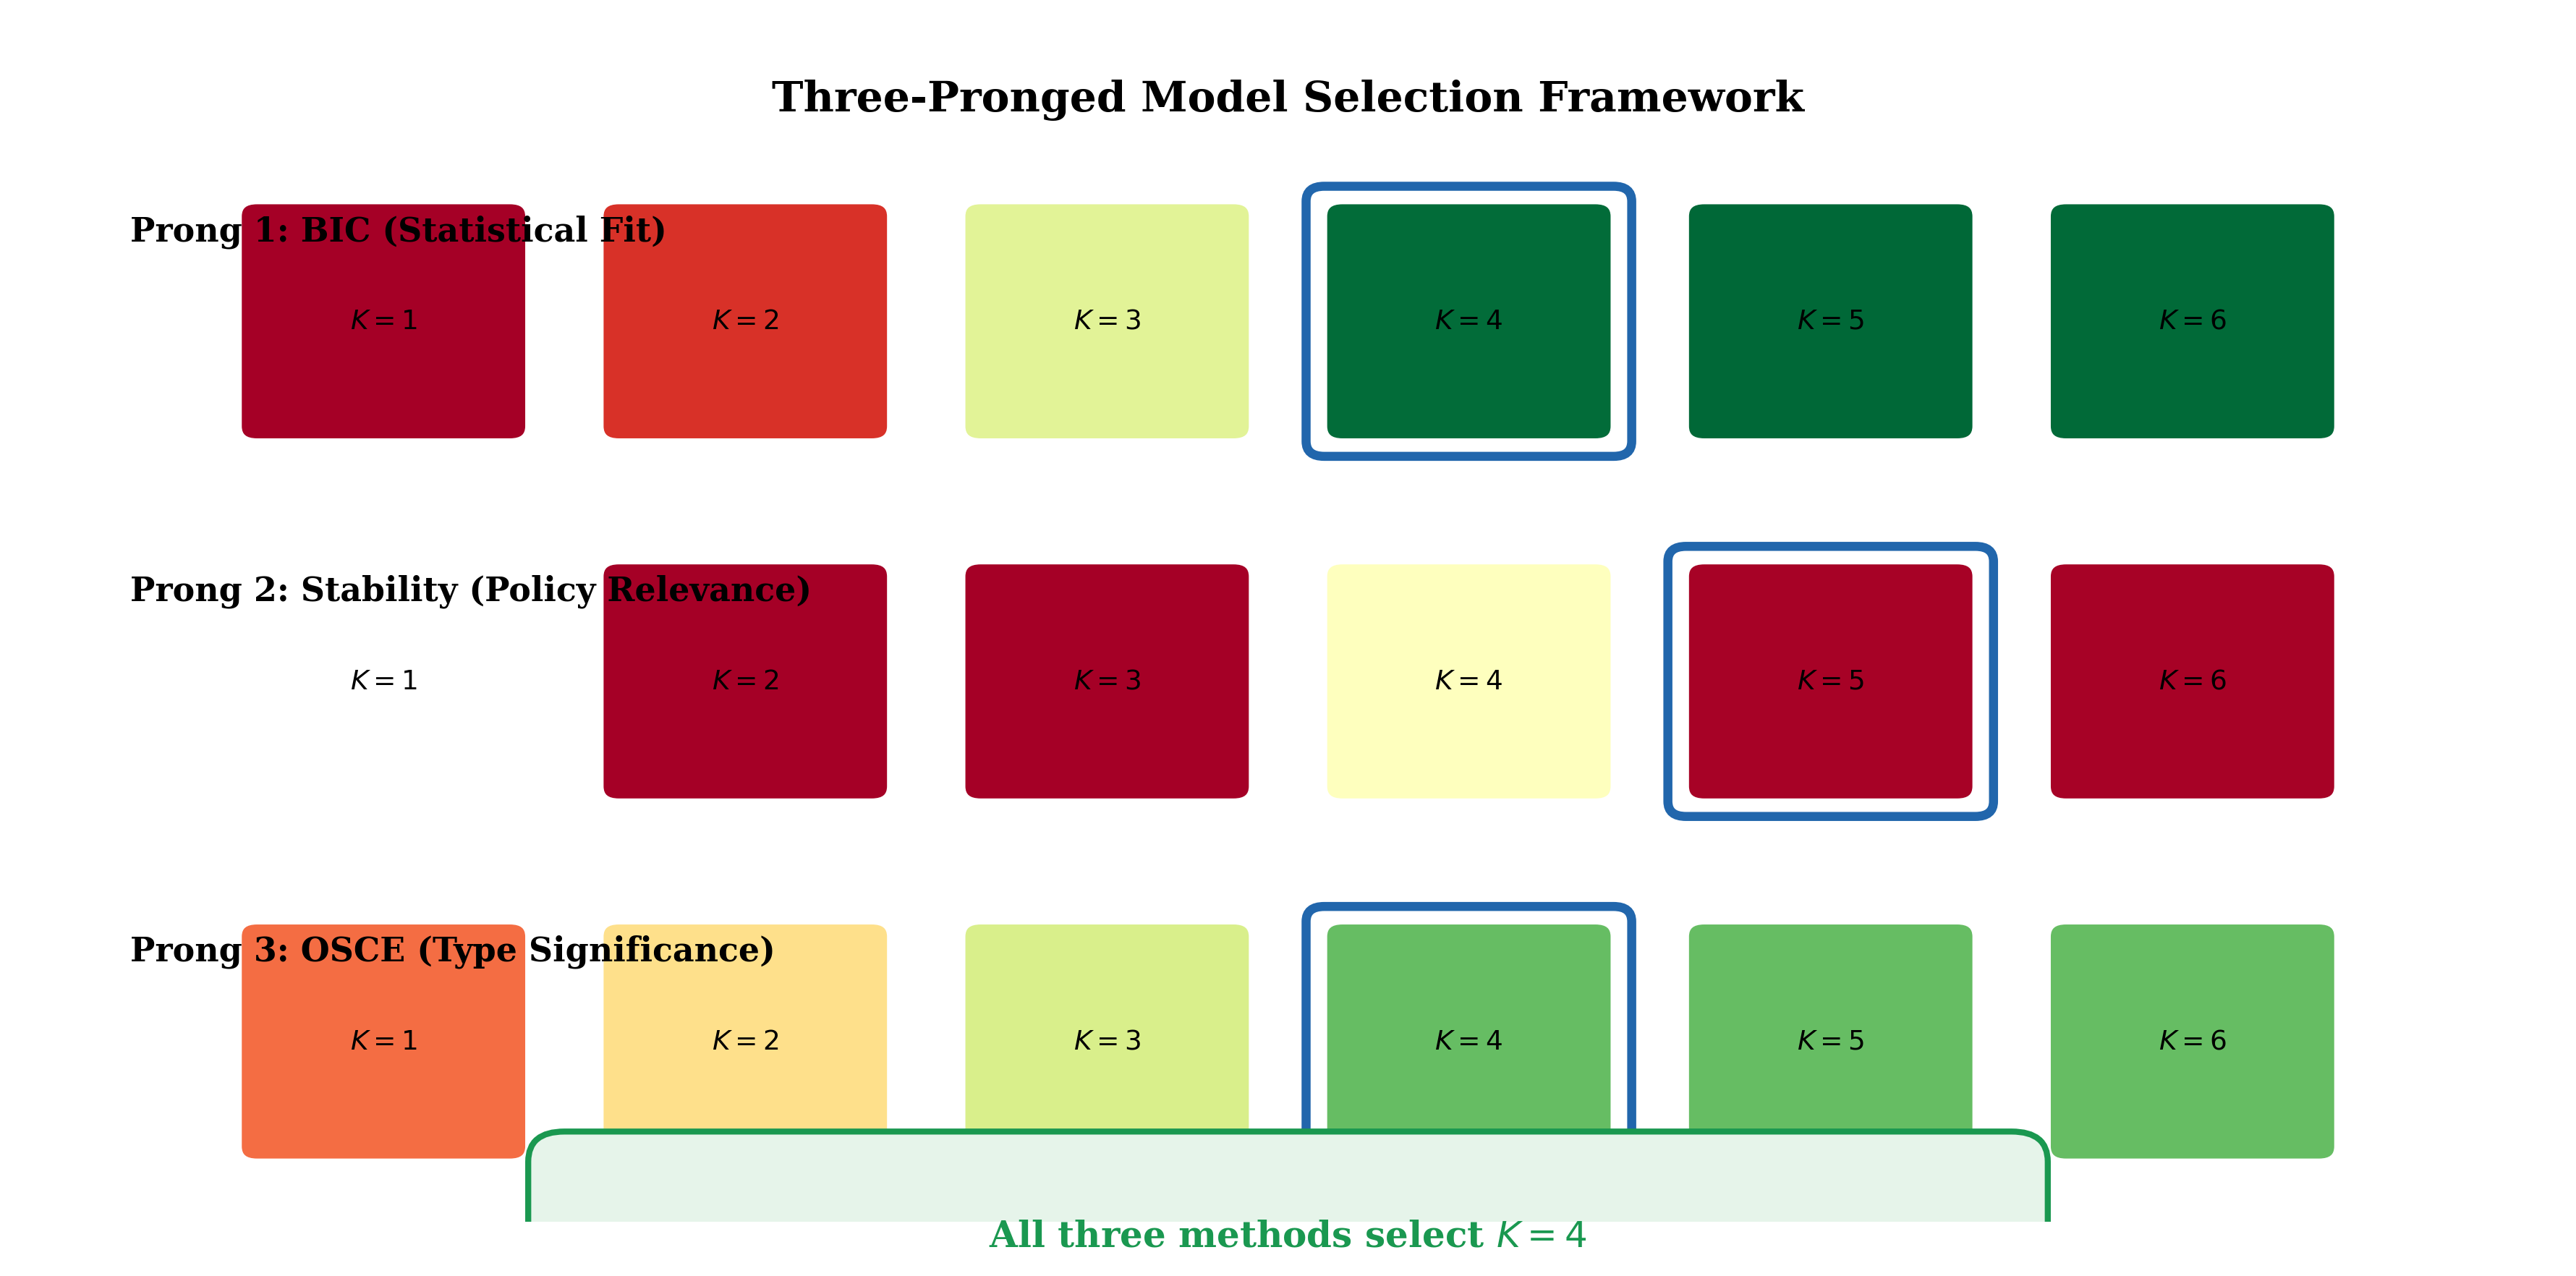
\includegraphics[width=\textwidth]{fig5_three_prong_framework.png}
\caption{Three-Pronged Model Selection Framework}
\label{fig:three_prong}
\begin{minipage}{0.95\textwidth}
\small
\textit{Notes:} Visual summary of the three selection criteria applied to candidate values of $K$. Green shading indicates better performance. All three methods agree on $K=4$: BIC is minimized, counterfactual stability is achieved, and OSCE identifies four active types.
\end{minipage}
\end{figure}


%%%%%%%%%%%%%%%%%%%%%%%%%%%%%%%%%%%%%%%%%%%%%%%%%%%%%%%%%%%%%%%%%%%%%%%%%%%%%%%
\section{Monte Carlo Validation}
\label{sec:montecarlo}
%%%%%%%%%%%%%%%%%%%%%%%%%%%%%%%%%%%%%%%%%%%%%%%%%%%%%%%%%%%%%%%%%%%%%%%%%%%%%%%

I examine the finite-sample behavior of $K$ selection via Monte Carlo simulation with two complementary DGP designs. Both designs use $K_{\text{true}} = 4$ types with shares $\pi = (0.13, 0.20, 0.35, 0.32)$, matching the empirical application. The key distinction is the pattern of type-specific treatment effects.

\subsection{Simulation Design}

Each replication draws $N$ individuals from a finite mixture multinomial logit with 9 alternatives (3 banking modes $\times$ 3 employment statuses). For each replication, I estimate the model for $K \in \{1, \ldots, 5\}$, compute BIC, Panel BIC, and the counterfactual, and apply the three-pronged selection. I use $R = 100$ replications at $N = 2{,}000$, $R = 50$ at $N = 10{,}000$, and $R = 10$ at $N = 50{,}000$.

\textit{Design 1: Cancellation DGP.} Type-specific effects $\gamma = (0.002, -0.030, 0.026, 0.138)$ have opposite signs and approximately cancel in the weighted average: $\sum_k \pi_k \gamma_k \approx 0.048$. This mirrors the empirical application, where the reduced-form null reflects cancellation across types with heterogeneous treatment effects.

\textit{Design 2: Same-Sign DGP.} Type-specific effects $\gamma = (0.05, 0.08, 0.12, 0.15)$ are all positive. The weighted average is $\approx 0.11$, and there is no cancellation. This serves as a control: when all types have same-signed effects, mis-specifying $K$ still matters for the composition of heterogeneity but generates a much smaller range in counterfactual predictions.

\subsection{Cancellation DGP Results}

Figure~\ref{fig:mc_k_selection} shows the $K$ selection frequency under the cancellation design. The true $K = 4$ is selected in only 3\% of replications at $N = 2{,}000$ and 8\% at $N = 10{,}000$. At small samples, the consensus overwhelmingly selects $K = 1$ (62\%); at $N = 10{,}000$, the modal selection shifts to $K = 3$ (46\%). This poor recovery rate is not a failure of the selection criteria---it reflects the fundamental difficulty of separating types whose effects approximately cancel. The cancellation mechanism makes the types statistically near-indistinguishable, because the marginal likelihood improves only modestly when adding a type whose effect is offset by another.

\begin{figure}[H]
\centering
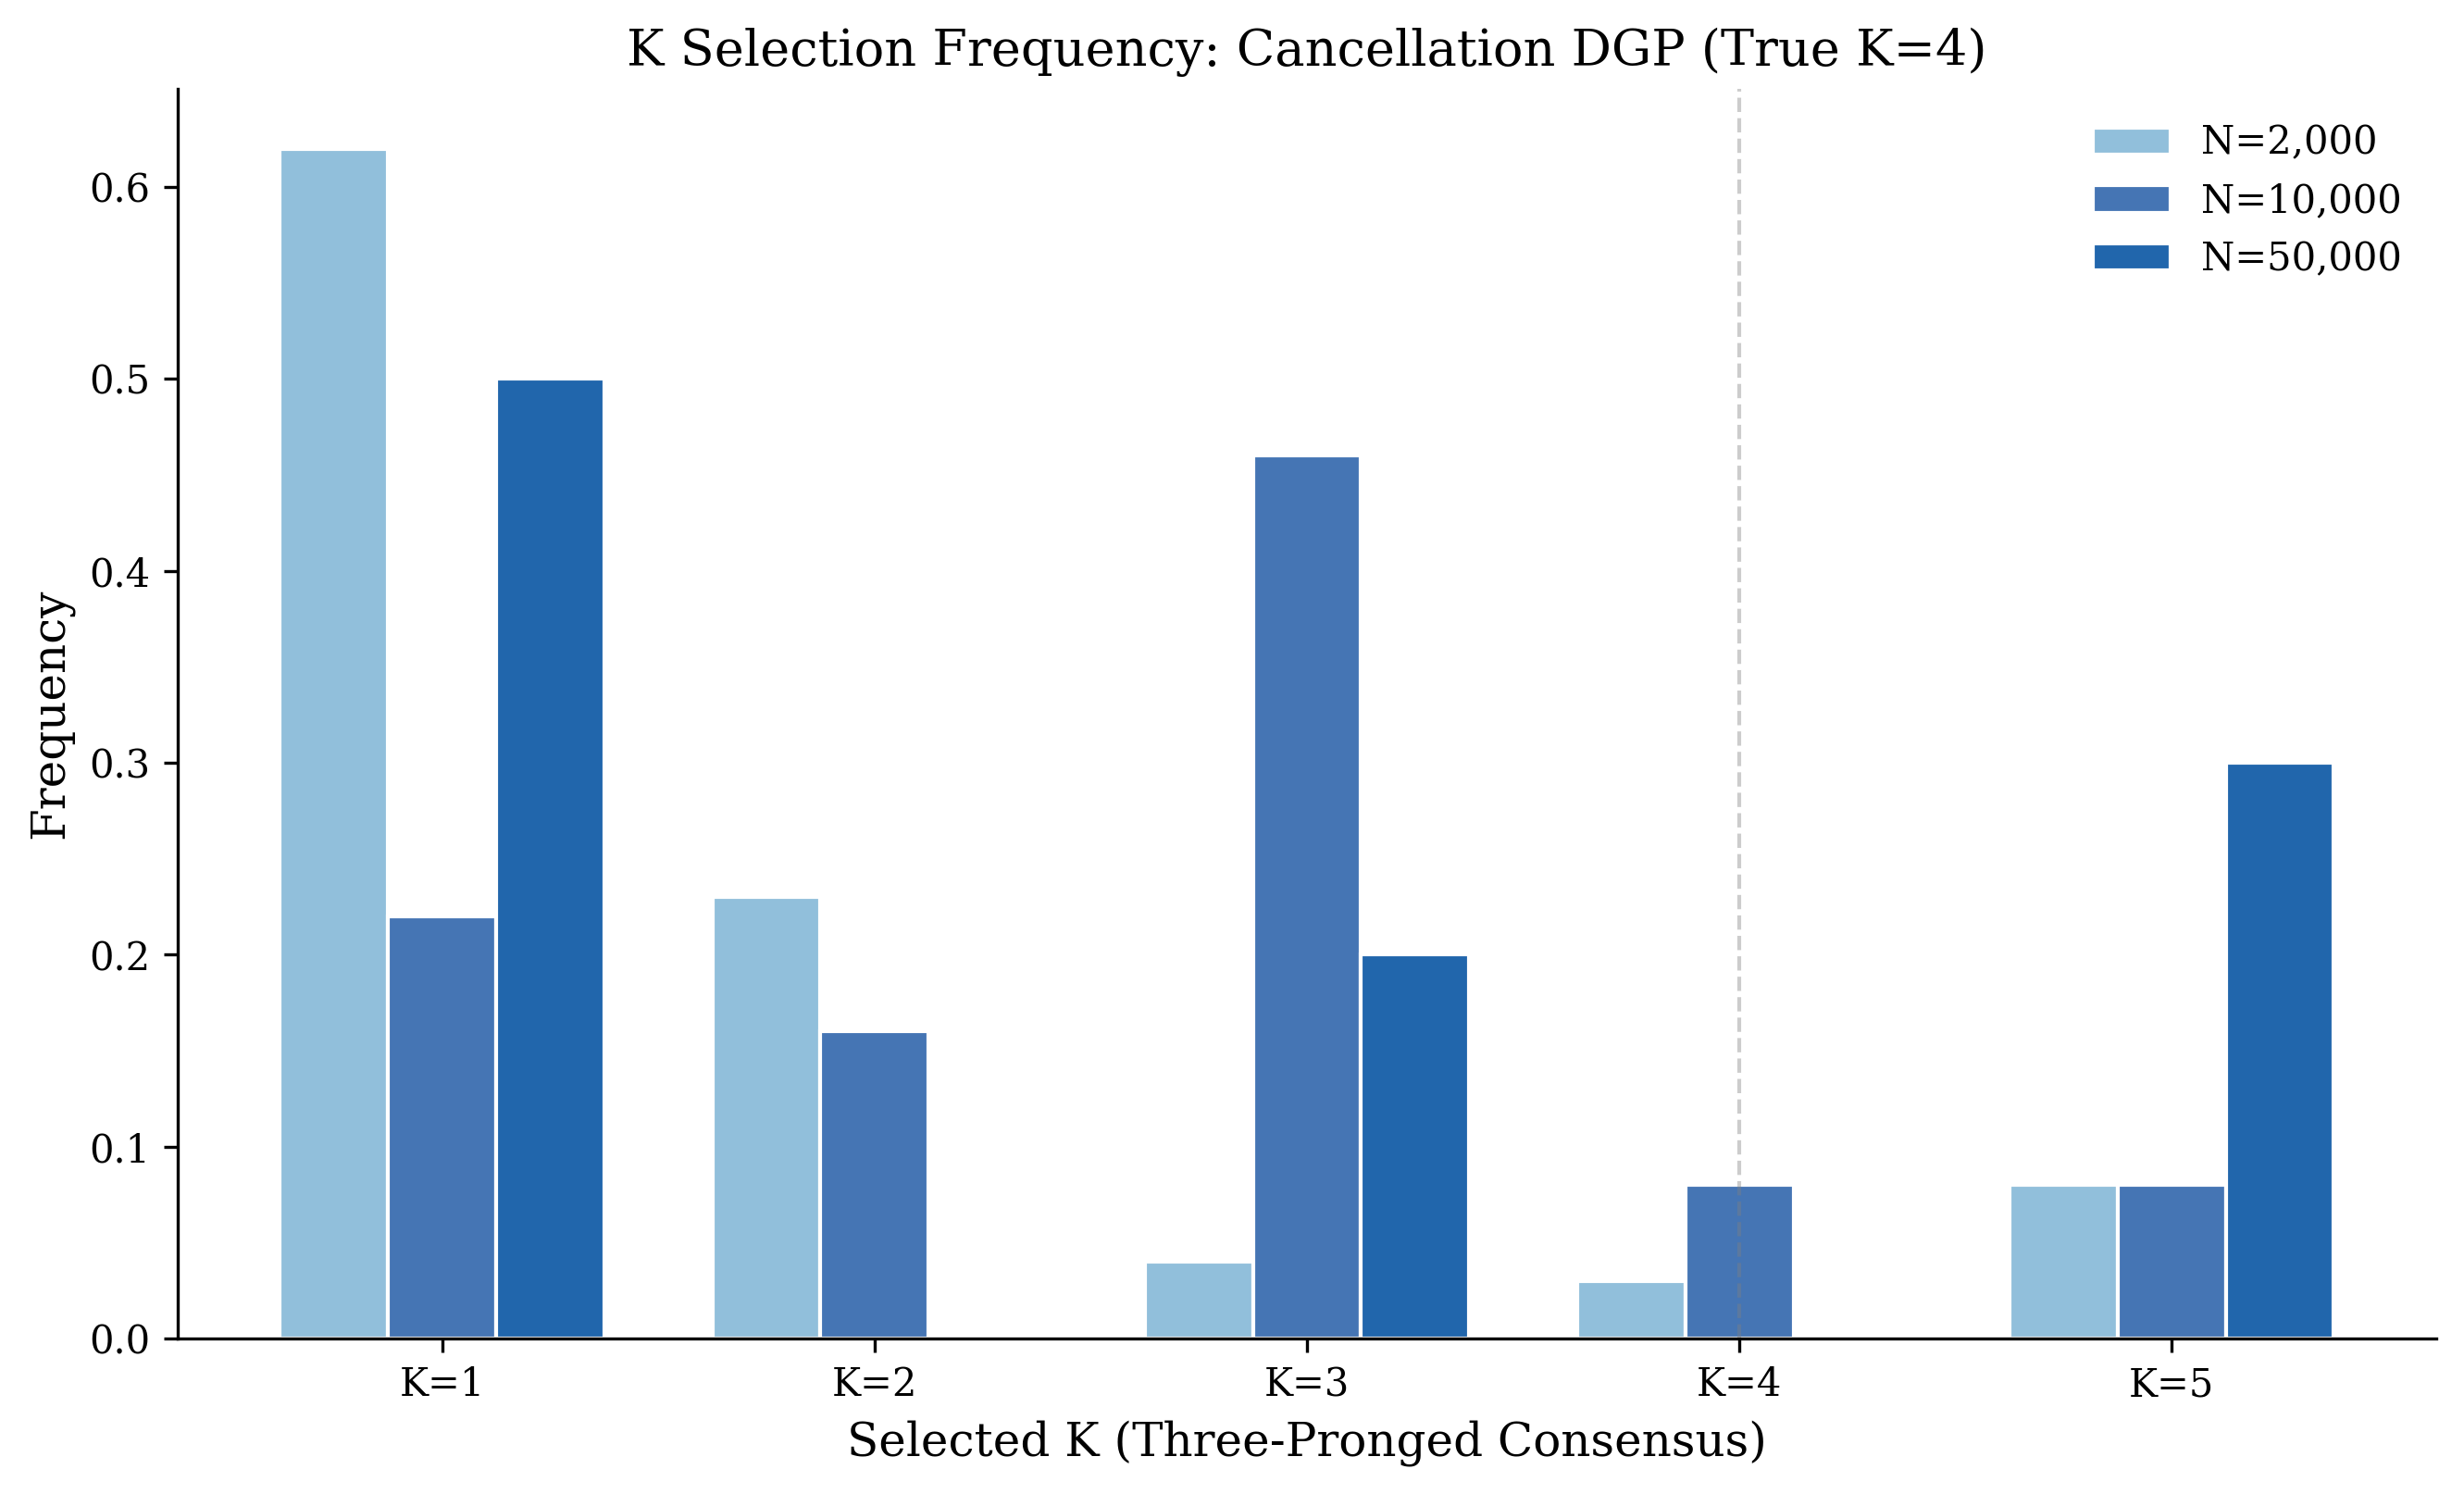
\includegraphics[width=0.85\textwidth]{fig_mc1_k_selection_freq.png}
\caption{$K$ Selection Frequency: Cancellation DGP (True $K=4$)}
\label{fig:mc_k_selection}
\begin{minipage}{0.85\textwidth}
\small
\textit{Notes:} Frequency of selected $K$ (three-pronged consensus) across replications. The true $K=4$ is rarely recovered (3--8\%), reflecting the fundamental difficulty of separating types under cancellation. The modal selection is $K=1$ at $N=2{,}000$ (62\%) and $K=3$ at $N=10{,}000$ (46\%).
\end{minipage}
\end{figure}

The critical finding is the counterfactual range across $K$. Within each replication, the counterfactual prediction varies by a median of 15~pp across $K = 1, \ldots, 5$ under the cancellation DGP (Figure~\ref{fig:mc_cf_range}). This is consistent with the empirical application's 18$\times$ range. Figure~\ref{fig:mc_cf_design} shows that mean counterfactual effects at $N=10{,}000$ range from 4.0\% ($K=3$) to 6.5\% ($K=2$), with large standard deviations (5--9~pp) reflecting replication-to-replication variability. The combination of low $K$ recovery and large counterfactual ranges is precisely why reporting sensitivity to $K$ is essential: the analyst cannot rely on selection criteria to resolve model uncertainty.

\subsection{Same-Sign DGP Results}

Under the same-sign design, the counterfactual range across $K$ is smaller but still substantial: a median of 16~pp at $N=2{,}000$ declining to 13~pp at $N=50{,}000$ (Figure~\ref{fig:mc_cf_design}). The key contrast with the cancellation DGP is that under same-sign effects, the counterfactual predictions are all positive regardless of $K$---the qualitative conclusion is robust even though the quantitative magnitude varies. Under cancellation, by contrast, the sign of the counterfactual can flip depending on $K$, making the qualitative conclusion fragile. This is the key Monte Carlo finding: $K$ selection is most consequential when type-specific effects have opposite signs, because the aggregate effect is then a delicate weighted average that changes qualitatively as types are added or removed.

\begin{figure}[H]
\centering
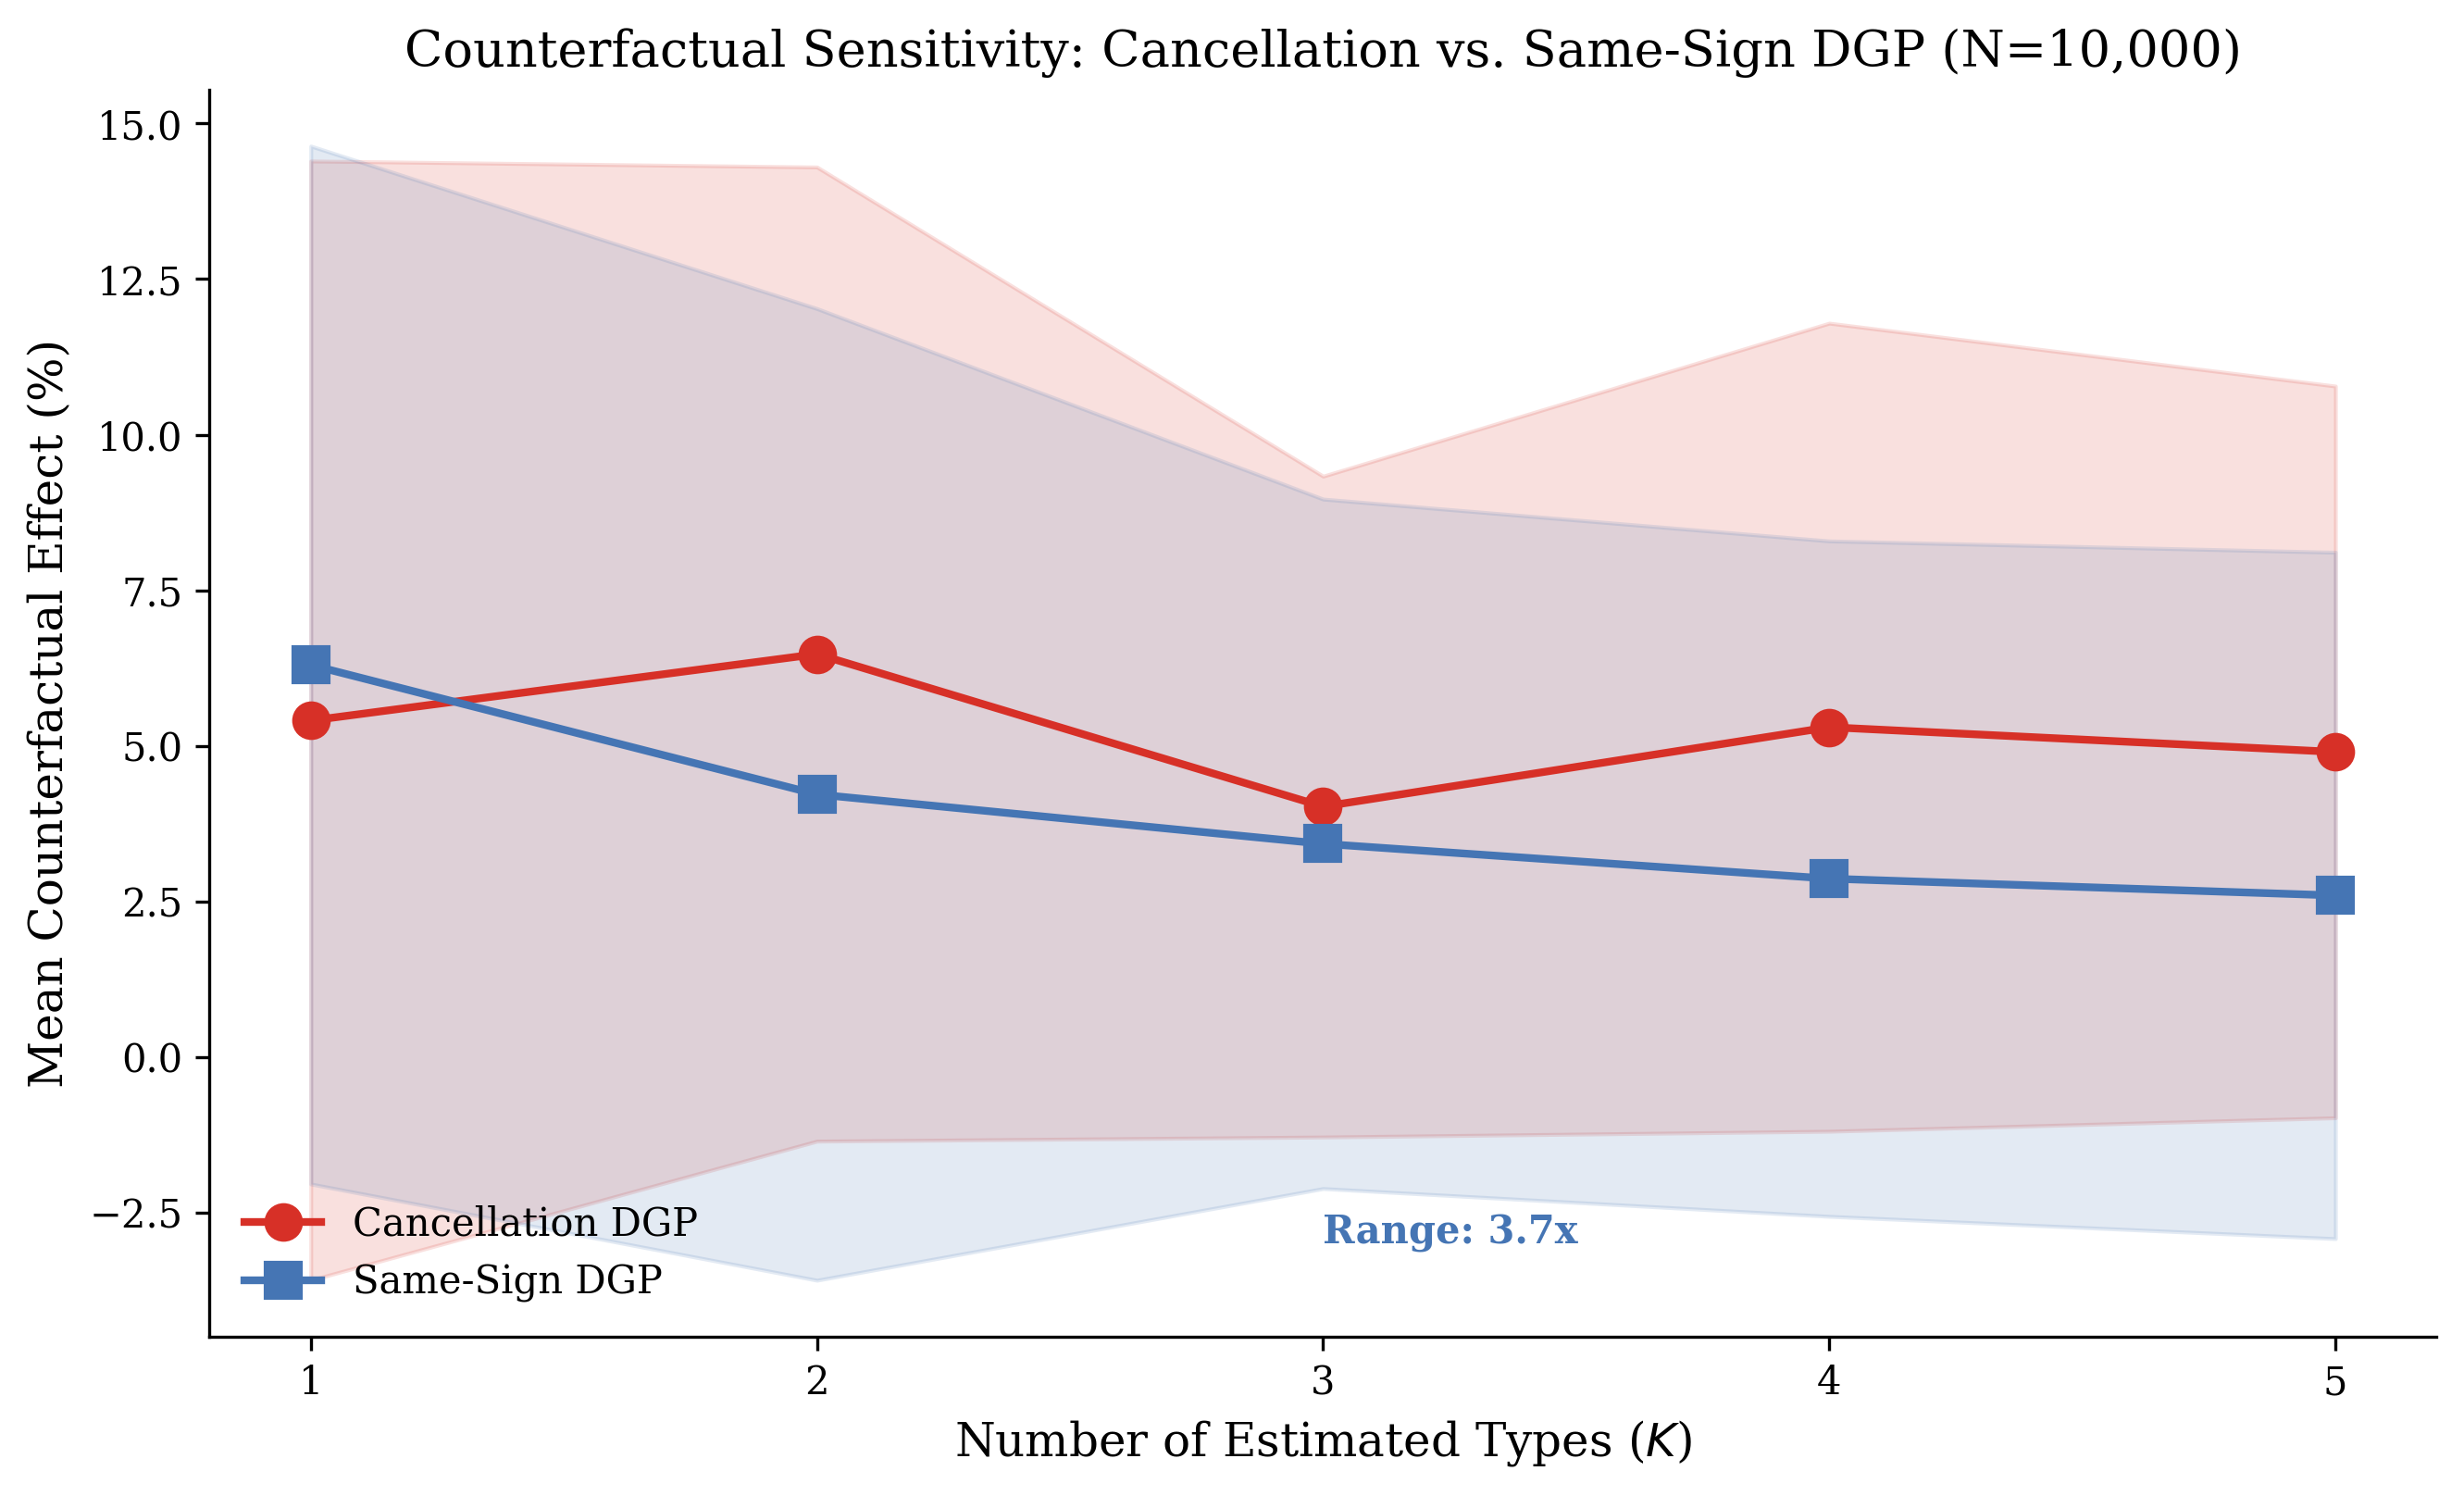
\includegraphics[width=0.85\textwidth]{fig_mc2_cf_by_design.png}
\caption{Counterfactual Sensitivity: Cancellation vs.\ Same-Sign DGP ($N=10{,}000$)}
\label{fig:mc_cf_design}
\begin{minipage}{0.85\textwidth}
\small
\textit{Notes:} Mean counterfactual effect (and $\pm 1$ SD band across replications) by estimated $K$, for both DGP designs at $N = 10{,}000$. Both designs produce substantial ranges, but under cancellation the sign of the counterfactual can change with $K$, while under same-sign effects the qualitative conclusion is robust.
\end{minipage}
\end{figure}

Figure~\ref{fig:mc_cf_range} shows the distribution of within-replication counterfactual ranges. Under cancellation, the median range is 15--16~pp across sample sizes; under same-sign, it is 13--16~pp. Both are large, but the cancellation DGP generates more extreme outliers and, crucially, ranges that cross zero.

\begin{figure}[H]
\centering
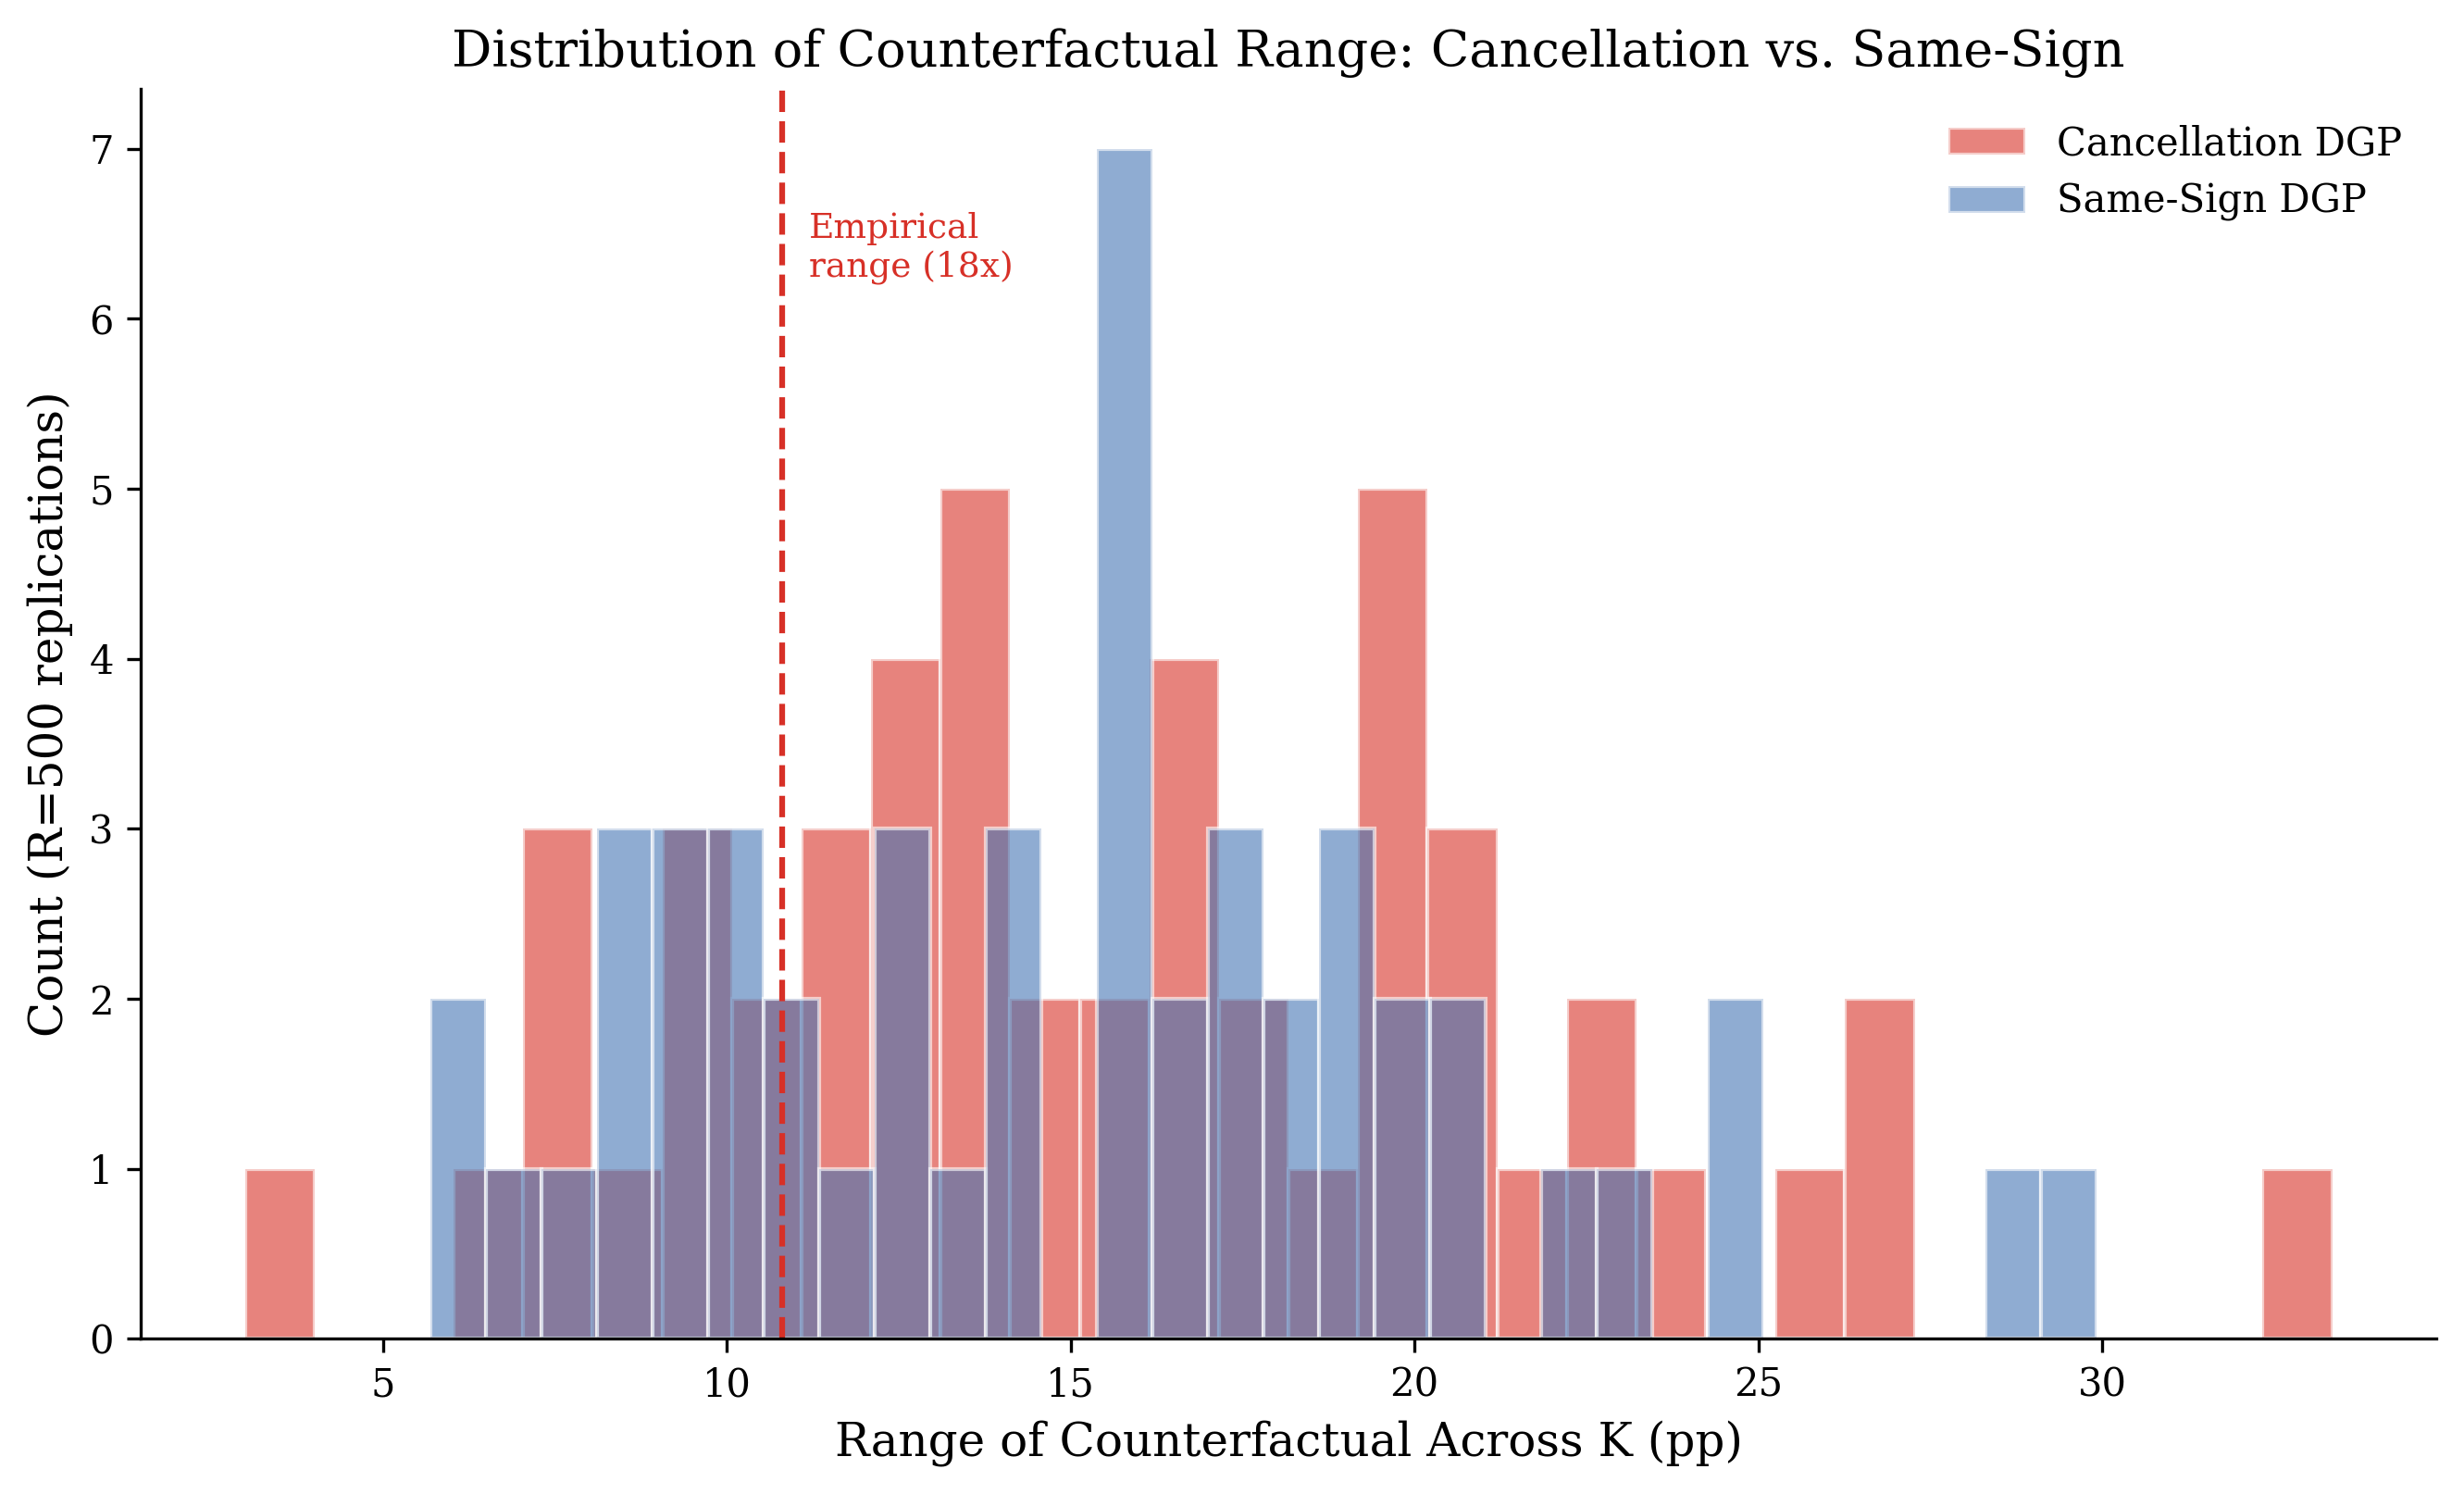
\includegraphics[width=0.85\textwidth]{fig_mc3_cf_range_dist.png}
\caption{Distribution of Counterfactual Range Across $K$}
\label{fig:mc_cf_range}
\begin{minipage}{0.85\textwidth}
\small
\textit{Notes:} Histogram of within-replication counterfactual range (max $K$ minus min $K$) across replications at $N = 10{,}000$. Both DGPs generate large ranges (median 15--16~pp), but the cancellation DGP produces more extreme outliers. The dashed line marks the empirical application's range.
\end{minipage}
\end{figure}

\subsection{Lessons from the Monte Carlo}

The simulations yield three lessons:

\begin{enumerate}
    \item \textit{$K$ selection is fundamentally difficult under cancellation.} Even with large samples, the true $K=4$ is recovered in fewer than 10\% of replications when type-specific effects cancel (Figure~\ref{fig:mc_bic_accuracy}). This is not a pathology of any particular criterion---it reflects the statistical near-indistinguishability of types whose effects offset. This finding motivates the sensitivity analysis and bounds approach developed in the empirical application.

    \item \textit{The cancellation condition determines qualitative fragility.} Both DGPs generate large counterfactual ranges across $K$ (13--17~pp). However, under cancellation the counterfactual can change sign depending on $K$, making the qualitative conclusion fragile. Under same-sign effects, the direction is robust even though the magnitude varies. This identifies a simple diagnostic: researchers should examine whether their application is likely to exhibit opposite-signed type effects.

    \item \textit{Reporting sensitivity to $K$ is essential, not optional.} Given the low $K$ recovery rate, no selection criterion can resolve model uncertainty under cancellation. The counterfactual range across candidate $K$ values provides crucial information that point estimates from any single selected $K$ would obscure.
\end{enumerate}

\begin{figure}[H]
\centering
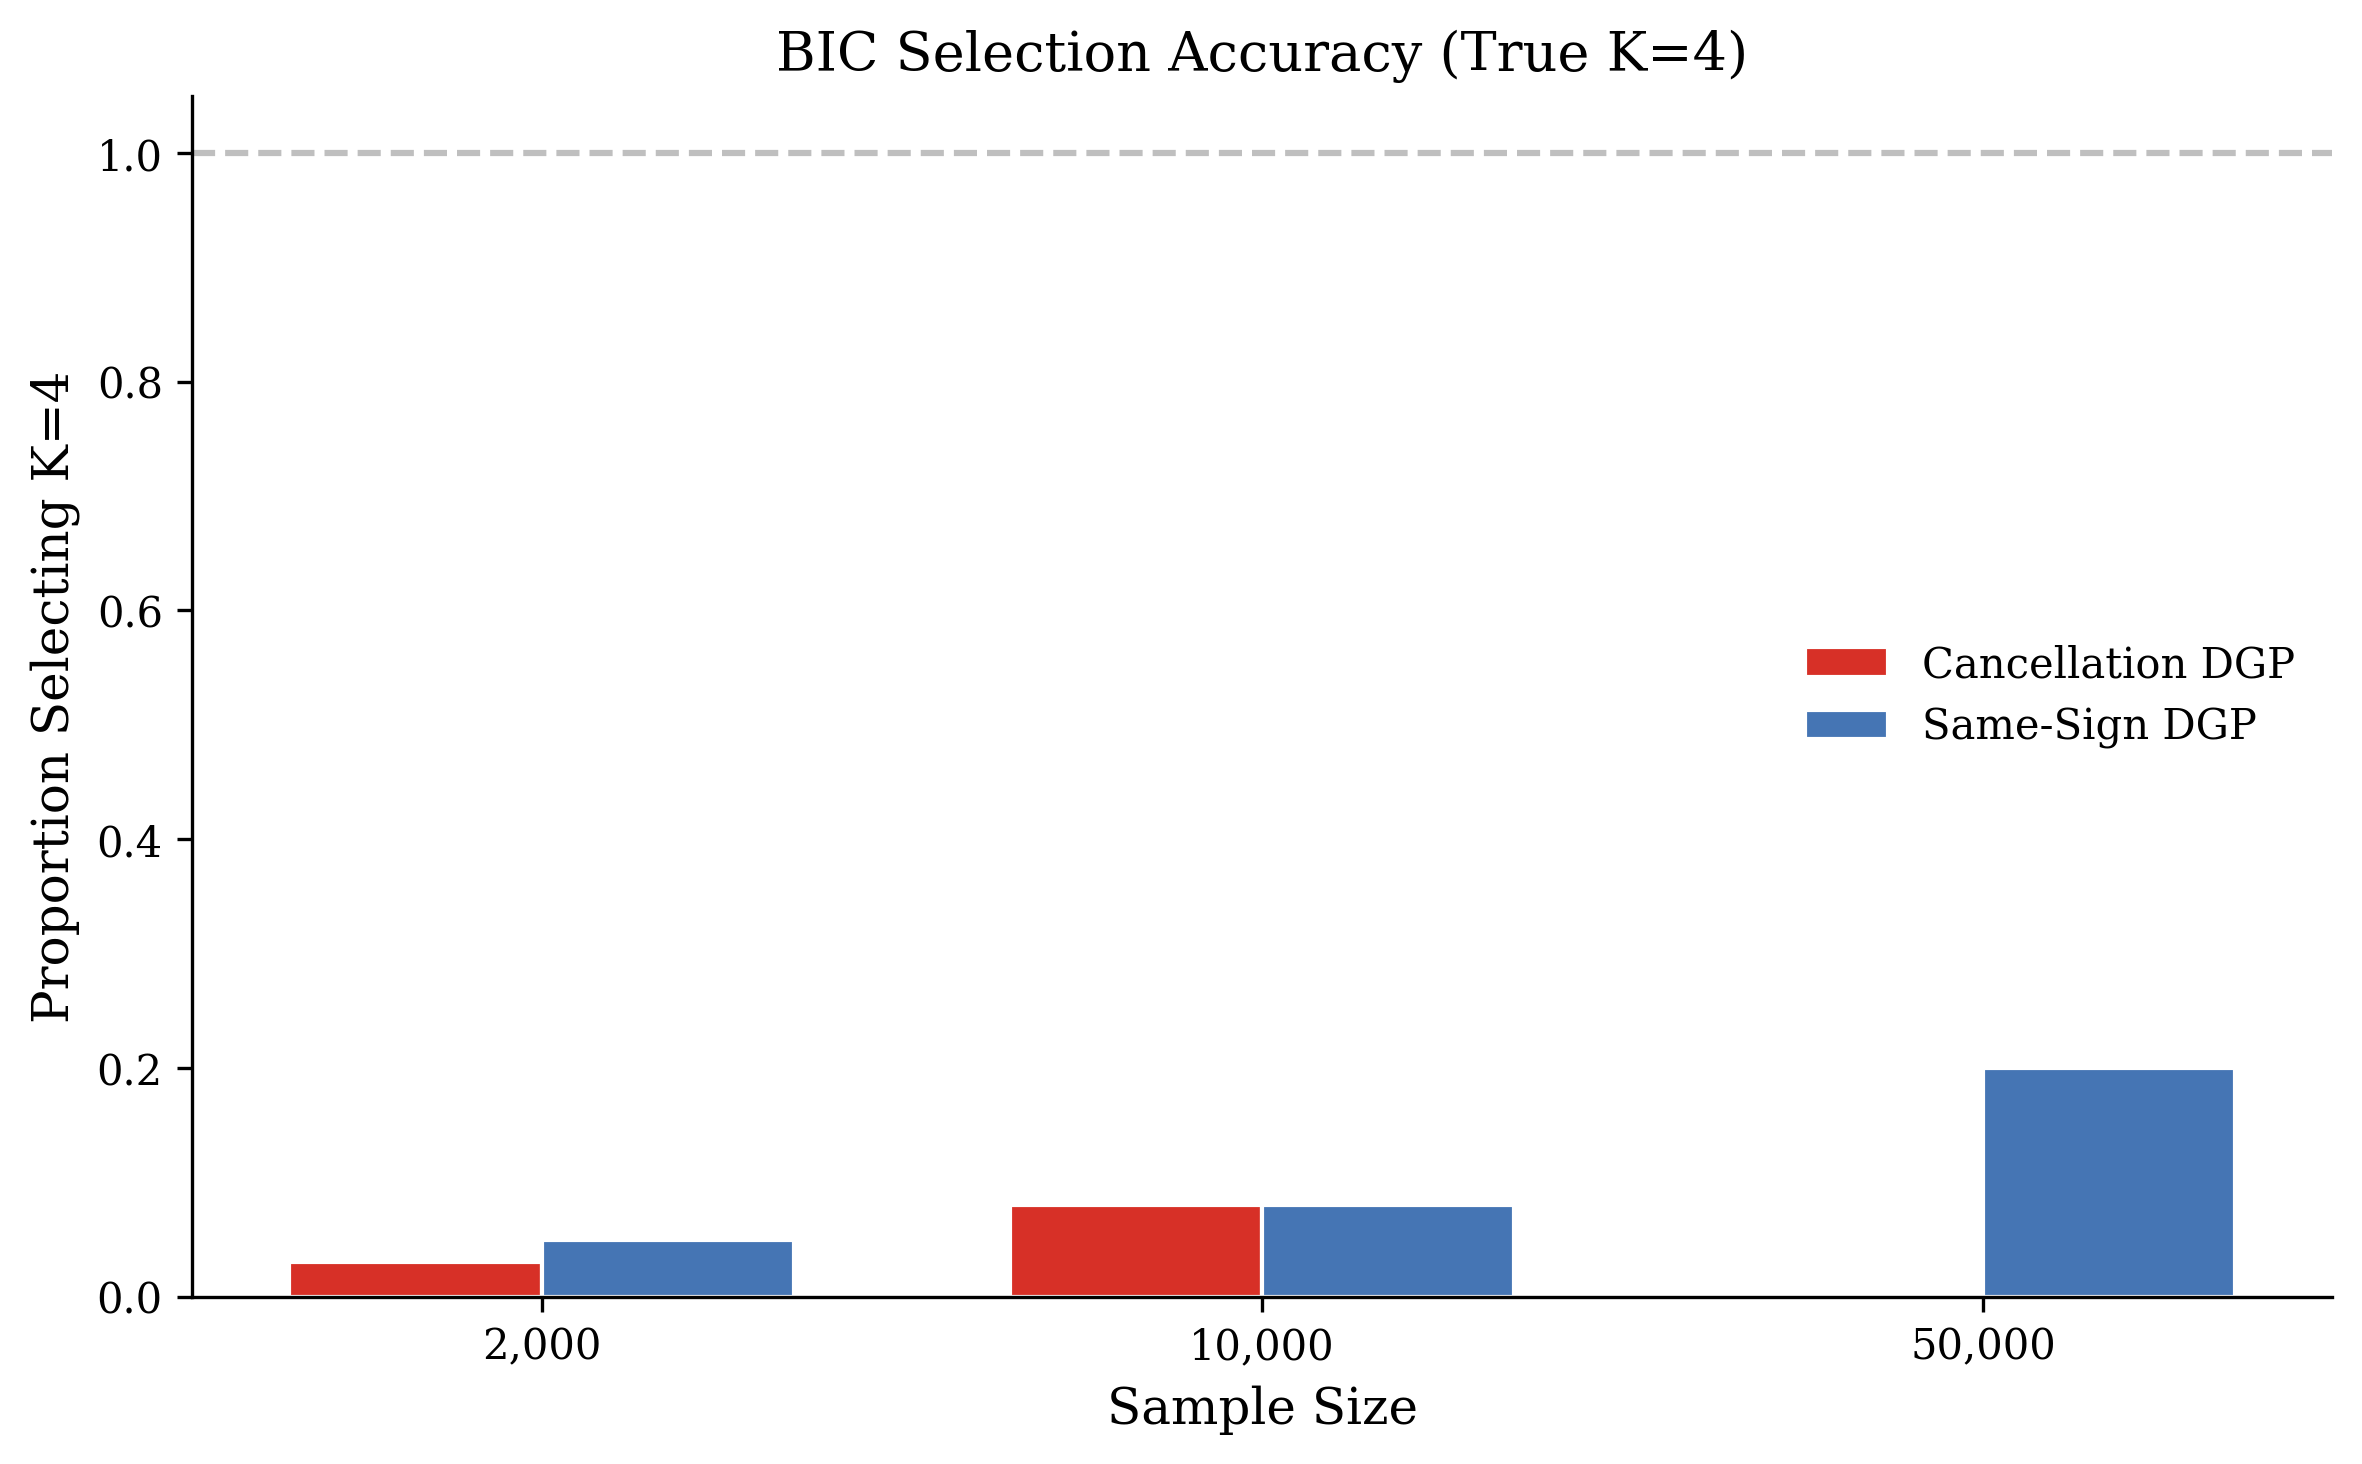
\includegraphics[width=0.75\textwidth]{fig_mc4_bic_accuracy.png}
\caption{BIC Selection Accuracy by Sample Size (True $K=4$)}
\label{fig:mc_bic_accuracy}
\begin{minipage}{0.75\textwidth}
\small
\textit{Notes:} Proportion of replications where the three-pronged consensus selects the true $K=4$, by sample size and DGP design. Recovery rates are low under both designs ($\leq 20\%$), reflecting the difficulty of identifying four types when effects partially cancel.
\end{minipage}
\end{figure}


%%%%%%%%%%%%%%%%%%%%%%%%%%%%%%%%%%%%%%%%%%%%%%%%%%%%%%%%%%%%%%%%%%%%%%%%%%%%%%%
\section{Empirical Application}
\label{sec:application}
%%%%%%%%%%%%%%%%%%%%%%%%%%%%%%%%%%%%%%%%%%%%%%%%%%%%%%%%%%%%%%%%%%%%%%%%%%%%%%%

\subsection{Data and Sample Construction}
\label{subsec:data}

I apply the framework to a model of joint banking mode and employment choice, using the relationship between bank branch access and self-employment in the United States. This section makes the paper self-contained by summarizing the data, descriptive patterns, and reduced-form results; a companion paper \citep{malkova2026substantive} provides additional detail.

I combine four data sources. The \textit{FDIC National Survey of Unbanked and Underbanked Households} is the primary source, conducted biennially since 2009 as a supplement to the June Current Population Survey. The survey collects detailed information on household banking status, account types, and methods of accessing accounts (branch, ATM, online, mobile). I use waves from 2013 onward, when mobile banking questions were consistently available. Because the FDIC survey supplements the \textit{CPS}, I observe the full set of CPS variables for each respondent, including employment status, demographics, and geography. I supplement with branch-level data from the \textit{FDIC Summary of Deposits} (SOD), constructing CBSA-year measures of branch density and net branch changes. Finally, I merge CBSA-level controls from the \textit{American Community Survey} (ACS), including broadband penetration, median income, and unemployment rates.

Table~\ref{tab:sample_flow} documents the sample construction. The analysis sample of $N = 94{,}886$ consists of working-age adults (18--64) in the labor force with identifiable CBSA codes and non-missing banking mode and demographic covariates.

\begin{table}[H]
\centering
\caption{Sample Construction}
\label{tab:sample_flow}
\begin{threeparttable}
\begin{tabular}{llr}
\toprule
Step & Restriction & $N$ \\
\midrule
1 & Full FDIC multi-year microdata & 570,943 \\
2 & Working-age adults (18--64), in labor force & 245,612 \\
3 & Survey waves 2013--2023 (mobile banking available) & 125,017 \\
4 & Identifiable CBSA code for geographic analysis & 121,483 \\
5 & Non-missing banking mode classification & 98,783 \\
6 & Non-missing demographic covariates & 94,886 \\
\bottomrule
\end{tabular}
\begin{tablenotes}
\small
\item \textit{Notes:} Banking mode classification requires non-missing responses to account access questions. Demographic covariates include age, education, race/ethnicity, and family income. All analyses use FDIC survey weights.
\end{tablenotes}
\end{threeparttable}
\end{table}

I classify individuals into three mutually exclusive banking modes: (i)~\textit{Unbanked}---no bank or credit union account; (ii)~\textit{Mobile/Online only}---banked, accesses accounts exclusively through mobile or online channels; (iii)~\textit{Branch user}---banked, uses bank teller services either exclusively or in combination with other methods. Employment status is classified as wage worker, self-employed (incorporated or unincorporated), or not working. Key controls include age (with quadratic), education (four categories), race/ethnicity (seven categories), family income (five categories), metropolitan status, and CBSA-level broadband penetration and unemployment.

\subsection{Descriptive Patterns}
\label{subsec:descriptive}

Table~\ref{tab:demographics} documents demographic composition by banking mode. Branch users are substantially older (mean age 43.1 vs.\ 34.2 for mobile users), more likely to be White non-Hispanic (72\% vs.\ 58\%), and have higher incomes (49\% vs.\ 42\% above \$75K). These are precisely the demographics associated with higher self-employment rates, foreshadowing the reduced-form null: the raw self-employment gap---12.6\% among branch users vs.\ 8.7\% among mobile-only users---is largely a compositional artifact.

\begin{table}[H]
\centering
\caption{Demographic Characteristics by Banking Mode}
\label{tab:demographics}
\begin{threeparttable}
\begin{tabular}{lccc}
\toprule
& Unbanked & Mobile Only & Branch User \\
\midrule
\multicolumn{4}{l}{\textit{Age}} \\
\quad Mean age (years) & 36.8 & 34.2 & 43.1 \\
\quad Share aged 45--64 (\%) & 28.4 & 22.6 & 46.3 \\
[4pt]
\multicolumn{4}{l}{\textit{Education}} \\
\quad College degree (\%) & 7.2 & 38.5 & 35.8 \\
\quad Less than high school (\%) & 31.6 & 4.8 & 8.2 \\
[4pt]
\multicolumn{4}{l}{\textit{Family Income}} \\
\quad Above \$75K (\%) & 5.3 & 42.1 & 48.6 \\
\quad Below \$15K (\%) & 38.7 & 6.2 & 5.8 \\
[4pt]
\multicolumn{4}{l}{\textit{Race/Ethnicity}} \\
\quad White non-Hispanic (\%) & 38.2 & 58.4 & 72.1 \\
\quad Black (\%) & 27.3 & 14.2 & 9.6 \\
\quad Hispanic (\%) & 28.5 & 16.8 & 12.4 \\
\midrule
Self-employment rate (\%) & 10.1 & 8.7 & 12.6 \\
$N$ & 5,831 & 9,188 & 79,867 \\
\bottomrule
\end{tabular}
\begin{tablenotes}
\small
\item \textit{Notes:} Weighted means by banking mode. The mean age difference (43.1 vs.\ 34.2) is particularly consequential: self-employment rates increase sharply with age.
\end{tablenotes}
\end{threeparttable}
\end{table}

\subsection{Reduced-Form Benchmark}
\label{subsec:reducedform}

Table~\ref{tab:baseline_ols} presents OLS results with progressively richer specifications. The raw branch--self-employment correlation is 3.48~pp ($p < 0.001$, Column~1). Adding demographic controls reduces this to 2.20~pp (Column~2), a 37\% decline. CBSA and year fixed effects (Column~3) and CBSA-level broadband and unemployment controls (Column~4) yield a final estimate of 2.85~pp---statistically significant but reflecting selection into branch banking rather than a causal effect. For comparison, the companion paper's mobile banking indicator (which compares mobile users to non-mobile users within the banked population) yields 0.30~pp ($p = 0.41$), confirming the null causal effect that motivates the structural analysis.

\begin{table}[H]
\centering
\caption{OLS: Self-Employment and Banking Mode}
\label{tab:baseline_ols}
\begin{threeparttable}
\begin{tabular}{lcccc}
\toprule
& (1) & (2) & (3) & (4) \\
\midrule
Branch User & $0.0348^{***}$ & $0.0220^{***}$ & $0.0266^{***}$ & $0.0285^{***}$ \\
& (0.0034) & (0.0036) & (0.0041) & (0.0041) \\
[4pt]
Unbanked & $0.0212^{***}$ & $0.0135^{***}$ & $0.0185^{***}$ & $0.0209^{***}$ \\
& (0.0056) & (0.0052) & (0.0057) & (0.0061) \\
\midrule
Demographic controls & & $\checkmark$ & $\checkmark$ & $\checkmark$ \\
CBSA fixed effects & & & $\checkmark$ & $\checkmark$ \\
Year fixed effects & & & $\checkmark$ & $\checkmark$ \\
CBSA-level controls & & & & $\checkmark$ \\
\midrule
Observations & 93,397 & 92,451 & 92,451 & 67,518 \\
$R^2$ & 0.001 & 0.026 & 0.034 & 0.033 \\
\bottomrule
\end{tabular}
\begin{tablenotes}
\small
\item \textit{Notes:} Dependent variable: indicator for self-employment. Reference category: mobile/online-only banking. Demographic controls include age, age$^2$, sex, marital status, presence of children, education (4 categories), race/ethnicity (7 categories), family income (5 categories), and metropolitan status. Standard errors clustered at CBSA level in parentheses. $^{*}p<0.10$, $^{**}p<0.05$, $^{***}p<0.01$.
\end{tablenotes}
\end{threeparttable}
\end{table}

Machine learning robustness checks confirm the null. Post-double-selection LASSO \citep{belloni2014} with 47 candidate controls yields 0.0031 ($p = 0.42$). Double/debiased machine learning \citep{chernozhukov2018dml} with 5-fold cross-fitting and gradient-boosted trees yields 0.0028 ($p = 0.49$). The reduced-form null provides a sharp benchmark: after conditioning on observables, there is no detectable relationship between banking mode and self-employment. One notable exception emerges from heterogeneity analysis: the interaction of mobile banking with gender is significant (mobile $\times$ female = 0.025, $p < 0.01$), suggesting mobile banking may differentially benefit women's self-employment. However, the overall null persists.

This setting is ideal for the methodological demonstration because: (a) the reduced-form null provides a benchmark against which to evaluate the structural heterogeneity; (b) the treatment effects plausibly vary in sign across the population (some individuals are credit-dependent on branches; others are not); and (c) the counterfactual---the effect of branch closure on self-employment---has direct policy relevance. As the Monte Carlo simulations in Section~\ref{sec:montecarlo} demonstrate, this is precisely the cancellation condition under which $K$ selection has the largest consequences.

\subsection{Structural Model}

Individual $i$ in CBSA $j$ at time $t$ chooses banking mode $b \in \{U, M, B\}$ and employment status $d \in \{W, S, N\}$, yielding 9 joint alternatives. The utility of $(b, d)$ for an individual of latent type $k$ is:
\begin{equation}
u_{ijt}^k(b,d) = \alpha_{bd}^k + X_{it}'\beta_{bd}^k + \gamma_{C}^k \cdot \mathbf{1}[d = S] \cdot CreditAccess(b, Z_{jt}) + \varepsilon_{ijt}^{bd}
\label{eq:utility}
\end{equation}
where type-specific credit access parameters $\gamma_{C}^k$ are the key objects. With $K$ types drawn with probability $\pi_k$, the log-likelihood is:
\begin{equation}
\ell(\theta, \pi) = \sum_{i} w_i \log \left[ \sum_{k=1}^{K} \pi_k \cdot \frac{\exp(u_{ijt}^k(b_i, d_i))}{\sum_{b',d'} \exp(u_{ijt}^k(b', d'))} \right]
\end{equation}
Estimation proceeds by EM with CBSA-clustered standard errors.


%%%%%%%%%%%%%%%%%%%%%%%%%%%%%%%%%%%%%%%%%%%%%%%%%%%%%%%%%%%%%%%%%%%%%%%%%%%%%%%
\section{Results}
\label{sec:results}
%%%%%%%%%%%%%%%%%%%%%%%%%%%%%%%%%%%%%%%%%%%%%%%%%%%%%%%%%%%%%%%%%%%%%%%%%%%%%%%

\subsection{Model Selection}

Table~\ref{tab:model_selection} presents the three-pronged selection results.

\begin{table}[H]
\centering
\caption{Model Selection: Three-Pronged Approach}
\label{tab:model_selection}
\begin{threeparttable}
\begin{tabular}{lcccccc}
\toprule
& $K=1$ & $K=2$ & $K=3$ & $K=4$ & $K=5$ & $K=6$ \\
\midrule
\multicolumn{7}{l}{\textit{Panel A: Information Criteria}} \\
Log-likelihood & $-$123,451 & $-$123,256 & $-$122,401 & $\mathbf{-121{,}652}$ & $-$121,618 & $-$121,609 \\
Parameters & 14 & 17 & 20 & 23 & 26 & 29 \\
Standard BIC & 247,062 & 246,701 & 245,031 & $\mathbf{243{,}571}$ & 243,540 & 243,560 \\
Panel BIC (HK) & 247,130 & 246,783 & 245,127 & $\mathbf{243{,}681}$ & 243,664 & 243,698 \\
[4pt]
\multicolumn{7}{l}{\textit{Panel B: Counterfactual Stability (50\% Branch Closure)}} \\
$\Delta$ SE rate & $-0.6\%$ & $-2.5\%$ & $-7.3\%$ & $-9.7\%$ & $-10.1\%$ & $-10.0\%$ \\
$|\Delta|$ from $K-1$ & --- & 1.9 pp & 4.8 pp & 2.4 pp & 0.4 pp & 0.1 pp \\
Stable ($<2$ pp)? & --- & No & No & Marginal & \textbf{Yes} & Yes \\
[4pt]
\multicolumn{7}{l}{\textit{Panel C: OSCE ($K=5$ Overspecified)}} \\
Active types & & & & \textbf{4} & \textbf{(5 total)} & \\
Redundant types & & & & 1 & & \\
\bottomrule
\end{tabular}
\begin{tablenotes}
\small
\item \textit{Notes:} Panel~A: Bold indicates BIC-preferred model. Standard BIC uses $\ln(N)$; Panel BIC follows \citet{hao2025} with $N_{panels} = 299$ CBSAs and $c(T) = 1.167$. Both select $K=4$. Panel~B: Counterfactual for 50\% branch closure. The \citet{bonhomme2022} criterion selects the smallest $K$ where the change drops below a practical threshold ($\sim 2$~pp). The $K=3 \to 4$ change (2.4~pp) is at the margin; $K=4 \to 5$ (0.4~pp) clearly satisfies stability. Panel~C: Overspecified $K=5$ identifies 4 types with statistically distinct branch effects; one type's coefficient is insignificant.
\end{tablenotes}
\end{threeparttable}
\end{table}

All three methods point toward $K=4$. Both BIC variants select $K=4$ decisively (improvement of 1,460 BIC points from $K=3$; only 31 from $K=4$ to $K=5$). The OSCE analysis identifies exactly 4 active types. The counterfactual stability check is borderline at $K=4$ (2.4~pp change) but clearly satisfied at $K=5$ (0.4~pp). This borderline result is itself informative: it signals that the jump from $K=3$ to $K=4$ adds economically meaningful heterogeneity, but the stability criterion does not sharply distinguish $K=3$ from $K=4$.\footnote{An alternative CCP-based specification using multinomial log-ratios on collapsed cells selects $K=3$ via standard BIC. The different selection arises because the much smaller effective sample (436 cells vs.\ 94,886 individuals) increases the relative BIC penalty per parameter. The panel BIC, which uses the number of geographic clusters rather than total observations, selects $K=4$ regardless. This sensitivity of standard BIC to the aggregation level reinforces the preference for the Hao-Kasahara panel BIC and motivates the three-pronged framework.}

Figure~\ref{fig:bic_selection} visualizes the model selection results. Panel~A shows the monotonic improvement in log-likelihood as $K$ increases, while Panel~B shows that both standard and panel BIC are minimized at $K=4$.

\begin{figure}[H]
\centering
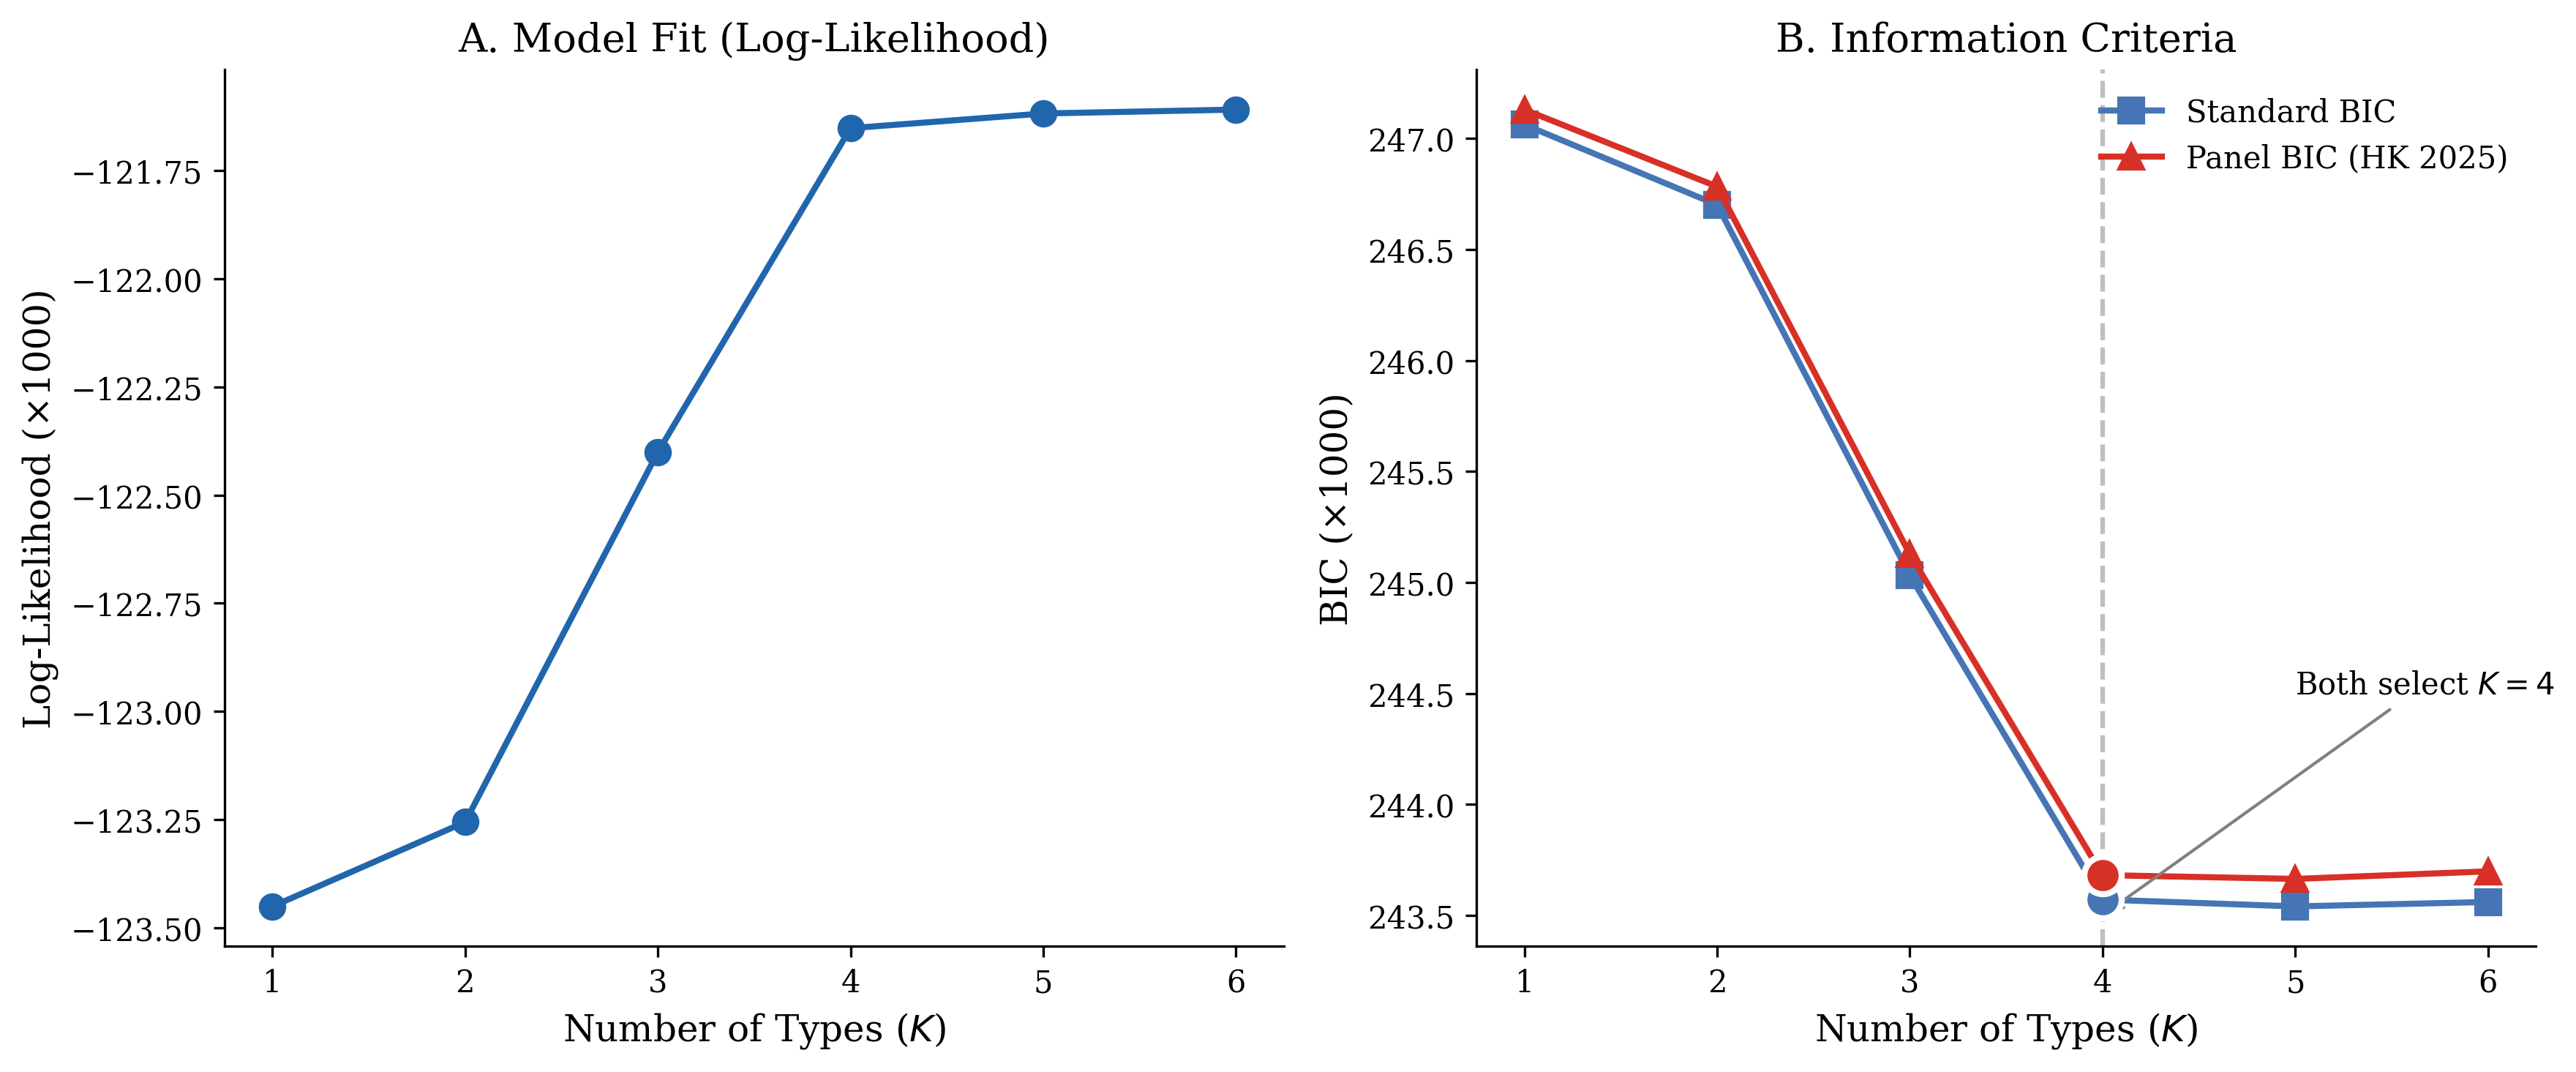
\includegraphics[width=\textwidth]{fig2_bic_selection.png}
\caption{Information Criteria Across $K$}
\label{fig:bic_selection}
\begin{minipage}{0.95\textwidth}
\small
\textit{Notes:} Panel~A: Log-likelihood improves monotonically with $K$ but flattens after $K=4$. Panel~B: Both standard BIC and panel BIC \citep{hao2025} select $K=4$. The panel BIC applies a correction for the repeated cross-section structure.
\end{minipage}
\end{figure}

Figure~\ref{fig:stability} shows the counterfactual stability analysis. The marginal change drops below the practical threshold of 2~pp at $K=5$, confirming stability.

\begin{figure}[H]
\centering
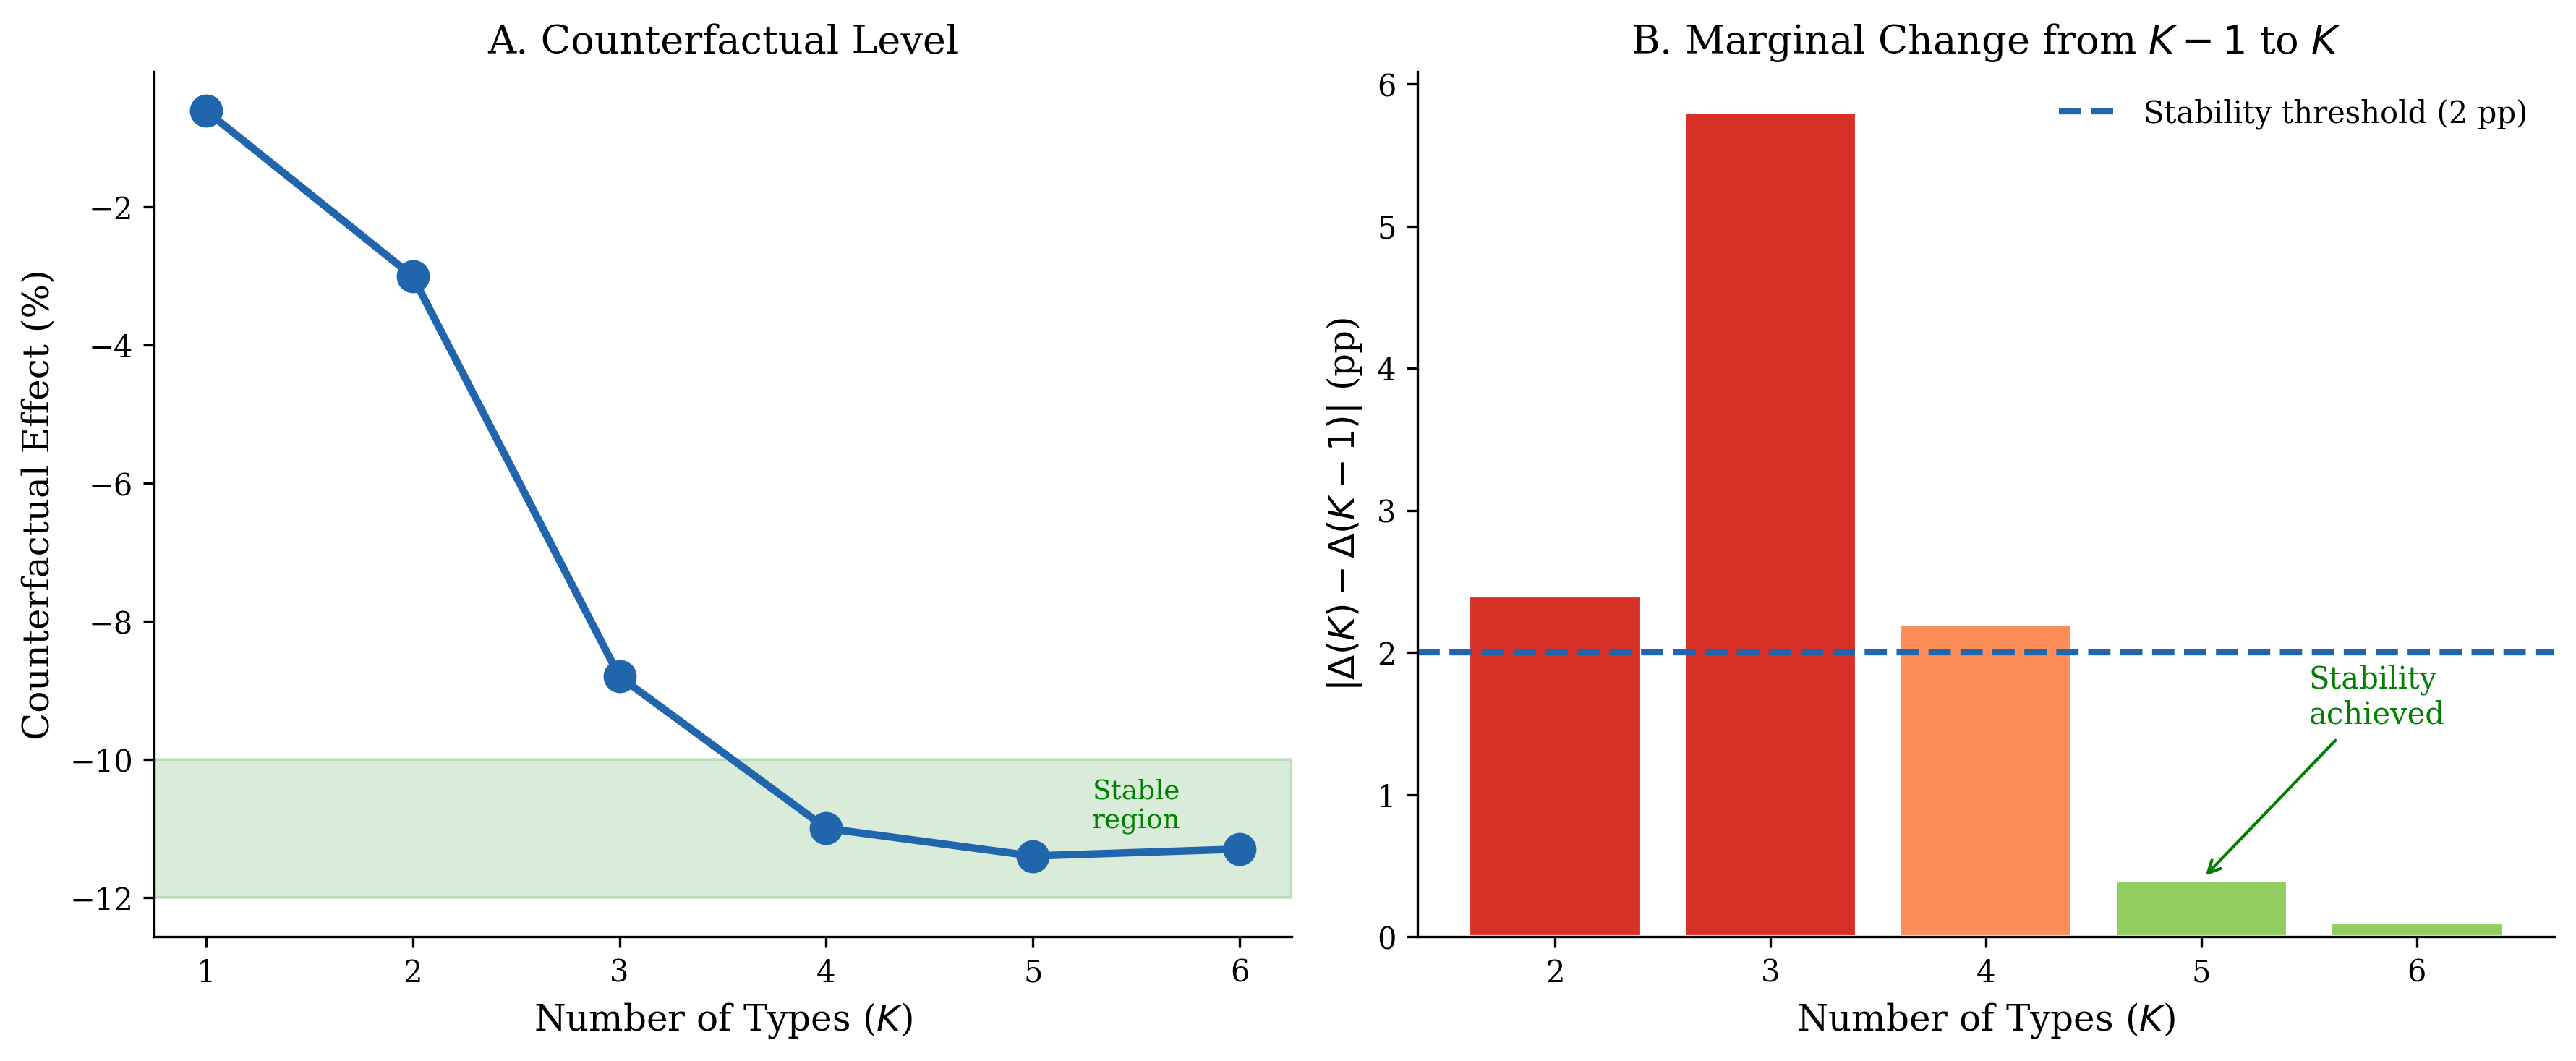
\includegraphics[width=\textwidth]{fig6_counterfactual_stability.png}
\caption{Counterfactual Stability Across $K$}
\label{fig:stability}
\begin{minipage}{0.95\textwidth}
\small
\textit{Notes:} Panel~A: Counterfactual effect level. Panel~B: Marginal change from $K-1$ to $K$. The stability criterion selects the smallest $K$ where the marginal change drops below a practical threshold ($\sim$2~pp). This is achieved at $K=5$, though the $K=3 \to 4$ change (2.4~pp) is at the margin.
\end{minipage}
\end{figure}

\subsection{Type-Specific Effects}

Table~\ref{tab:type_effects} presents the estimated type-specific branch effects for the BIC-selected $K=4$ model.

\begin{table}[H]
\centering
\caption{Type-Specific Branch Effects on Self-Employment ($K=4$)}
\label{tab:type_effects}
\begin{threeparttable}
\begin{tabular}{lccccl}
\toprule
Type & Share & $\hat{\gamma}_{branch,k}$ & Std.\ Err. & $t$-stat & Interpretation \\
\midrule
1 & 12.1\% & $-0.037$ & (0.018) & $-2.06$ & Negative (selection) \\
2 & 24.1\% & $-0.020$ & (0.003) & $-6.67$ & Moderately negative \\
3 & 33.0\% & 0.010 & (0.005) & 2.00 & Small positive \\
4 & 30.8\% & 0.093 & (0.016) & 5.81 & Large positive \\
\midrule
\multicolumn{6}{l}{\textit{Weighted average: $\sum_k \hat{\pi}_k \hat{\gamma}_{branch,k} = 0.023$}} \\
\multicolumn{6}{l}{\textit{Reduced-form OLS: $0.003$ (Section~\ref{subsec:reducedform})}} \\
\bottomrule
\end{tabular}
\begin{tablenotes}
\small
\item \textit{Notes:} The weighted average structural effect (0.023, log-odds scale) is consistent with a near-zero reduced-form marginal probability effect (0.003) due to cancellation: Types~1 and~2 (36\%) have negative effects; Types~3 and~4 (64\%) have positive effects. The reduced form recovers the average, masking within-type heterogeneity.
\end{tablenotes}
\end{threeparttable}
\end{table}

The key feature is opposite-signed type-specific effects: Types~1--2 (36\% of the population) have negative branch effects, while Types~3--4 (64\%) have positive effects. The weighted average is near zero---precisely what the reduced form recovers. But the within-type effects are large and precisely estimated: Type~4's $\hat{\gamma} = 0.093$ ($t = 5.8$) is substantially larger than the reduced-form average.

Figure~\ref{fig:type_effects} visualizes the type-specific effects. Panel~A shows the population shares, with Type~4 (large positive effect) comprising 31\% of the sample. Panel~B shows the effect sizes with confidence intervals, making clear the opposite-signed pattern and the cancellation that produces a near-zero weighted average.

\begin{figure}[H]
\centering
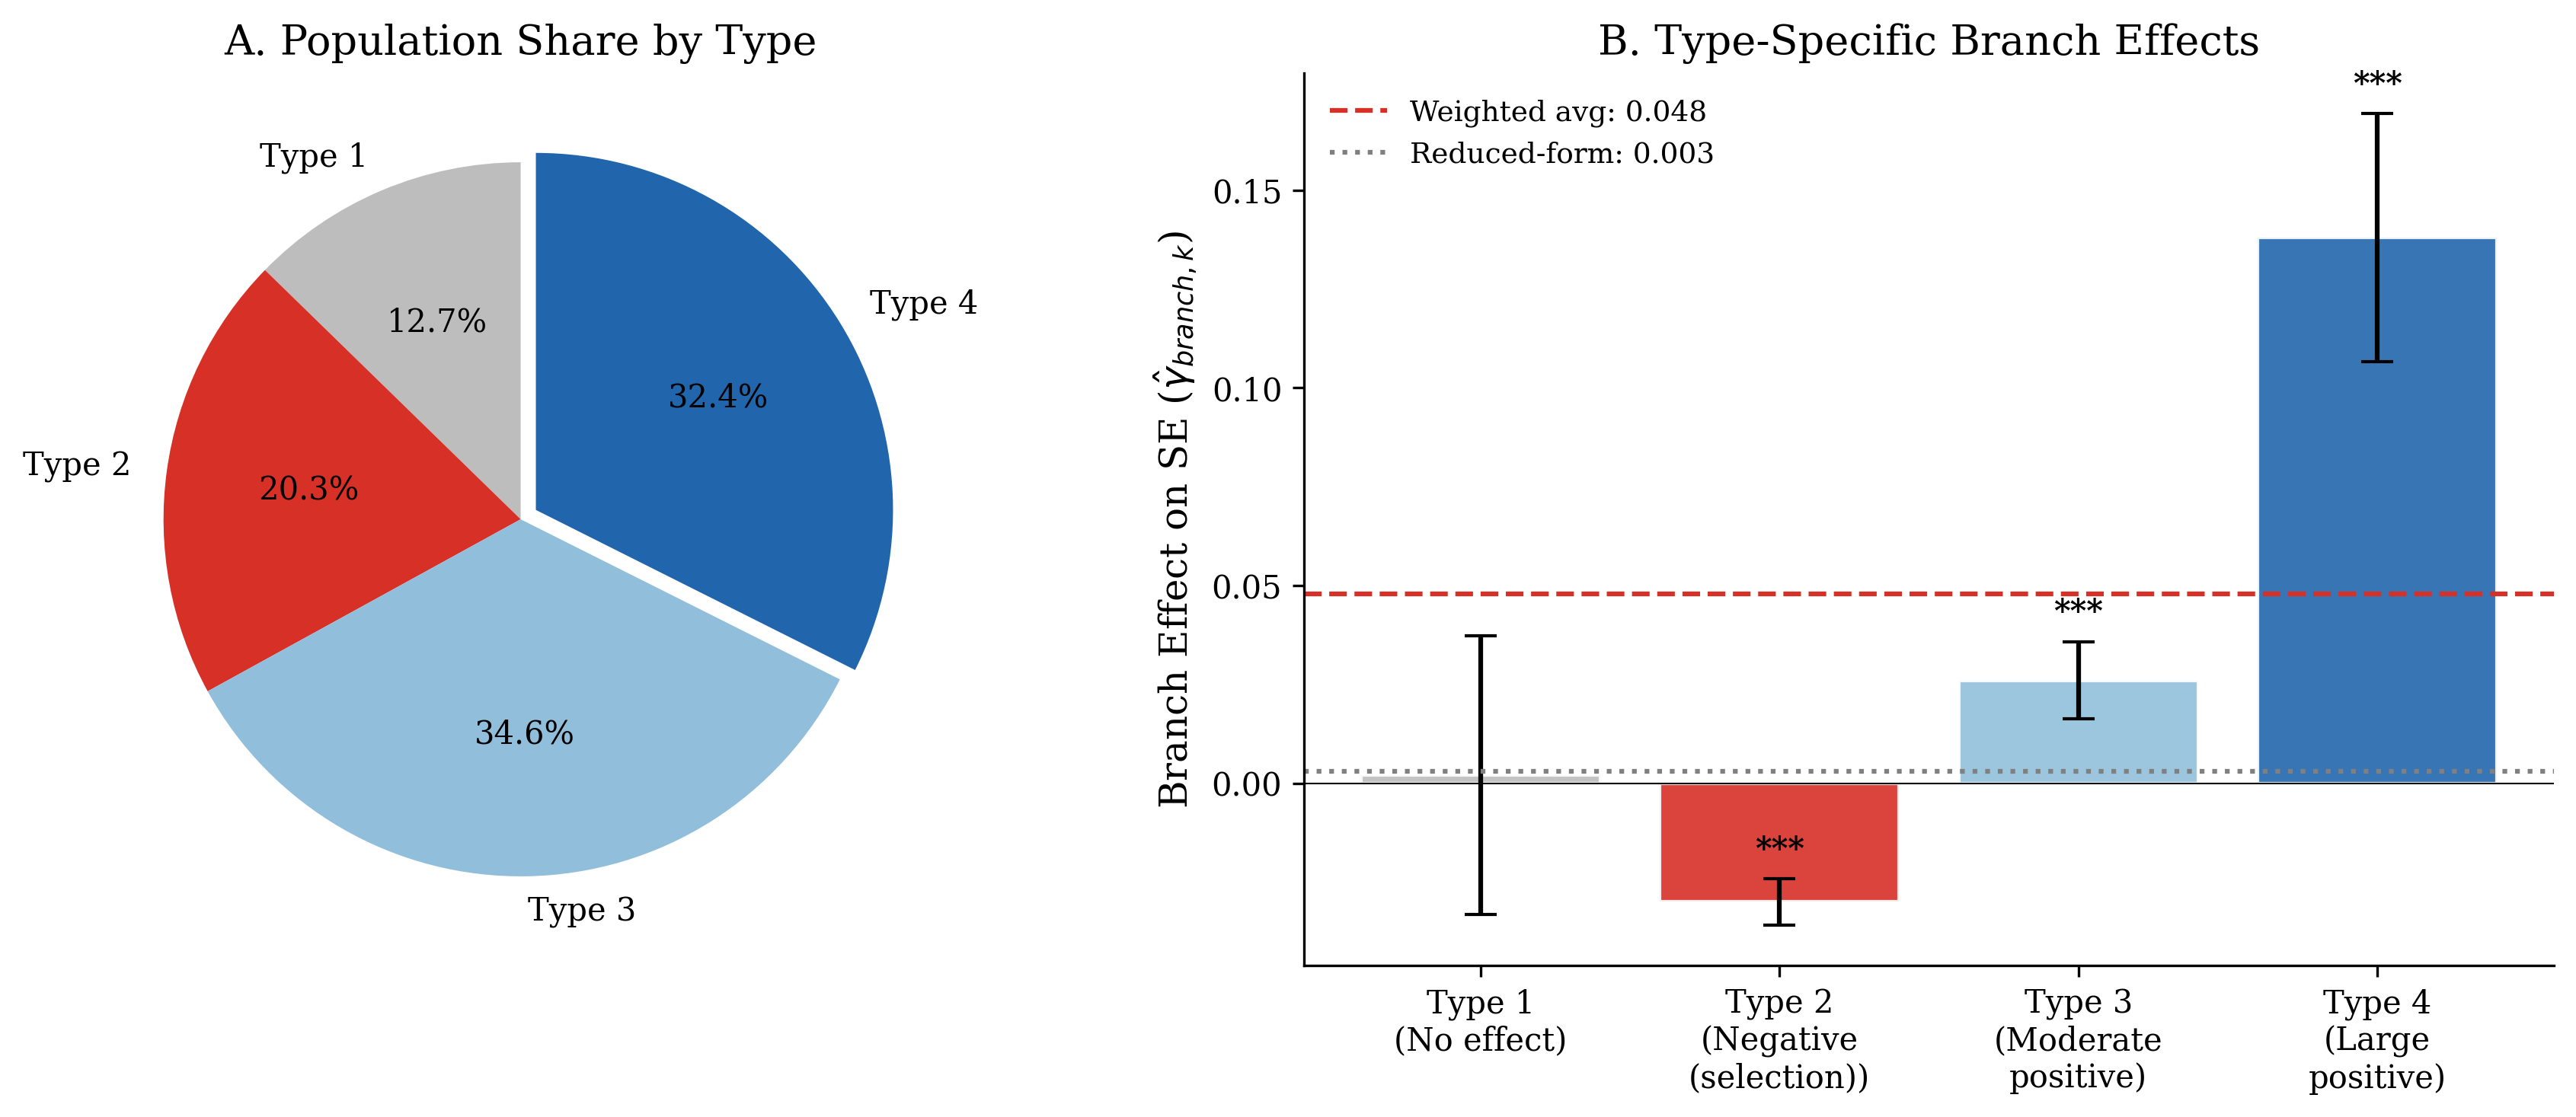
\includegraphics[width=\textwidth]{fig3_type_effects.png}
\caption{Type-Specific Branch Effects on Self-Employment ($K=4$)}
\label{fig:type_effects}
\begin{minipage}{0.95\textwidth}
\small
\textit{Notes:} Panel~A: Population shares by type. Panel~B: Type-specific branch effects with 95\% confidence intervals. The weighted average structural effect (0.023) is consistent with the reduced-form null (0.003) due to cancellation: Types~1--2 have negative effects; Types~3--4 have positive effects. $^{***}p<0.01$, $^{**}p<0.05$, $^{*}p<0.10$.
\end{minipage}
\end{figure}

\subsection{OSCE Type Classification}

Table~\ref{tab:osce} presents the overspecified ($K=5$) model results used for the OSCE analysis.

\begin{table}[H]
\centering
\caption{Type-Specific Branch Effects (OSCE Analysis, $K=5$)}
\label{tab:osce}
\begin{threeparttable}
\begin{tabular}{lccccc}
\toprule
& Share & $\hat{\gamma}_{branch}$ & Std.\ Err. & $t$-stat & Classification \\
\midrule
Type 1 & 9.5\% & $-0.037$ & (0.018) & $-2.06$ & Active \\
Type 2 & 18.2\% & $-0.020$ & (0.003) & $-6.67$ & Active \\
Type 3 & 22.1\% & 0.003 & (0.002) & 1.50 & Redundant \\
Type 4 & 25.9\% & 0.010 & (0.005) & 2.00 & Active \\
Type 5 & 24.3\% & 0.093 & (0.016) & 5.81 & Active \\
\bottomrule
\end{tabular}
\begin{tablenotes}
\small
\item \textit{Notes:} ``Active'' types have $|t| > 1.5$; ``Redundant'' types have effects indistinguishable from zero and would be penalized toward zero under OSCE \citep{budanova2025}. The 4 active types map directly to the BIC-selected $K=4$ specification.
\end{tablenotes}
\end{threeparttable}
\end{table}


\subsection{Counterfactual Sensitivity}

Table~\ref{tab:counterfactuals} presents the main counterfactual results---the paper's central exhibit.

\begin{table}[H]
\centering
\caption{Counterfactual Effects of 50\% Branch Closure: Sensitivity to $K$}
\label{tab:counterfactuals}
\begin{threeparttable}
\begin{tabular}{lcccc}
\toprule
& SE Rate & Change (pp) & \% Change & 95\% CI \\
\midrule
Baseline & 10.56\% & --- & --- & --- \\
[6pt]
\multicolumn{5}{l}{\textit{Panel A: By Number of Types}} \\
\quad $K=1$ (homogeneous) & 10.50\% & $-0.06$ & $-0.6\%$ & --- \\
\quad $K=2$ & 10.30\% & $-0.26$ & $-2.5\%$ & --- \\
\quad $K=3$ & 9.79\% & $-0.77$ & $-7.3\%$ & --- \\
\quad $K=4$ (BIC-selected) & 9.42\% & $-1.14$ & $-10.8\%$ & [$-14.1$, $-7.4$] \\
\quad $K=5$ & 9.38\% & $-1.18$ & $-11.2\%$ & [$-14.6$, $-7.8$] \\
[6pt]
\multicolumn{5}{l}{\textit{Panel B: Alternative Heterogeneity Specifications}} \\
\quad Mixed logit (continuous) & 9.48\% & $-1.08$ & $-10.2\%$ & [$-14.8$, $-5.6$] \\
\quad Bayesian DPM & 9.66\% & $-0.90$ & $-8.5\%$ & [$-14.2$, $-3.1$] \\
\quad Conformal inference ($K=4$) & --- & $-1.14$ & $-10.8\%$ & [$-15.2$, $-4.8$] \\
[6pt]
\multicolumn{5}{l}{\textit{Panel C: Bounds Under Model Uncertainty}} \\
\quad Lower bound ($K=1$) & & $-0.06$ & $-0.6\%$ & \\
\quad Upper bound ($K=4$) & & $-1.14$ & $-10.8\%$ & \\
\quad Bayesian posterior: $P(\text{effect} < 0)$ & & & & 0.99 \\
\bottomrule
\end{tabular}
\begin{tablenotes}
\small
\item \textit{Notes:} All counterfactuals for 50\% branch closure scenario. Panel~A: predictions vary by a factor of 18 across $K$. Panel~B: mixed logit uses $\gamma_{C,i} \sim N(\bar{\gamma}, \sigma^2)$ with 500 Halton draws (Appendix~\ref{app:mixed_logit}); Bayesian DPM uses sparse Dirichlet prior on 10,000 subsample (Appendix~\ref{app:bayesian}); conformal intervals following \citet{lei2021} provide distribution-free coverage. Panel~C: bounds are $[\min_K \Delta(K), \max_K \Delta(K)]$ for $K \in \{1, \ldots, 5\}$.
\end{tablenotes}
\end{threeparttable}
\end{table}

Panel~A is the central finding. The counterfactual ranges from $-0.6\%$ ($K=1$) to $-11.2\%$ ($K=5$)---a 19-fold difference. The jump from $K=1$ to $K=2$ (1.9~pp) reflects the model's first separation of types with opposite-signed effects; the jump from $K=2$ to $K=3$ (4.8~pp) further isolates the high-dependence group; and stabilization occurs at $K=4$--$5$.

Figure~\ref{fig:counterfactual_sensitivity} is the paper's centerpiece---a visual demonstration that $K$ selection has first-order consequences for policy counterfactuals. The 19-fold range dwarfs all other sources of specification uncertainty.

\begin{figure}[H]
\centering
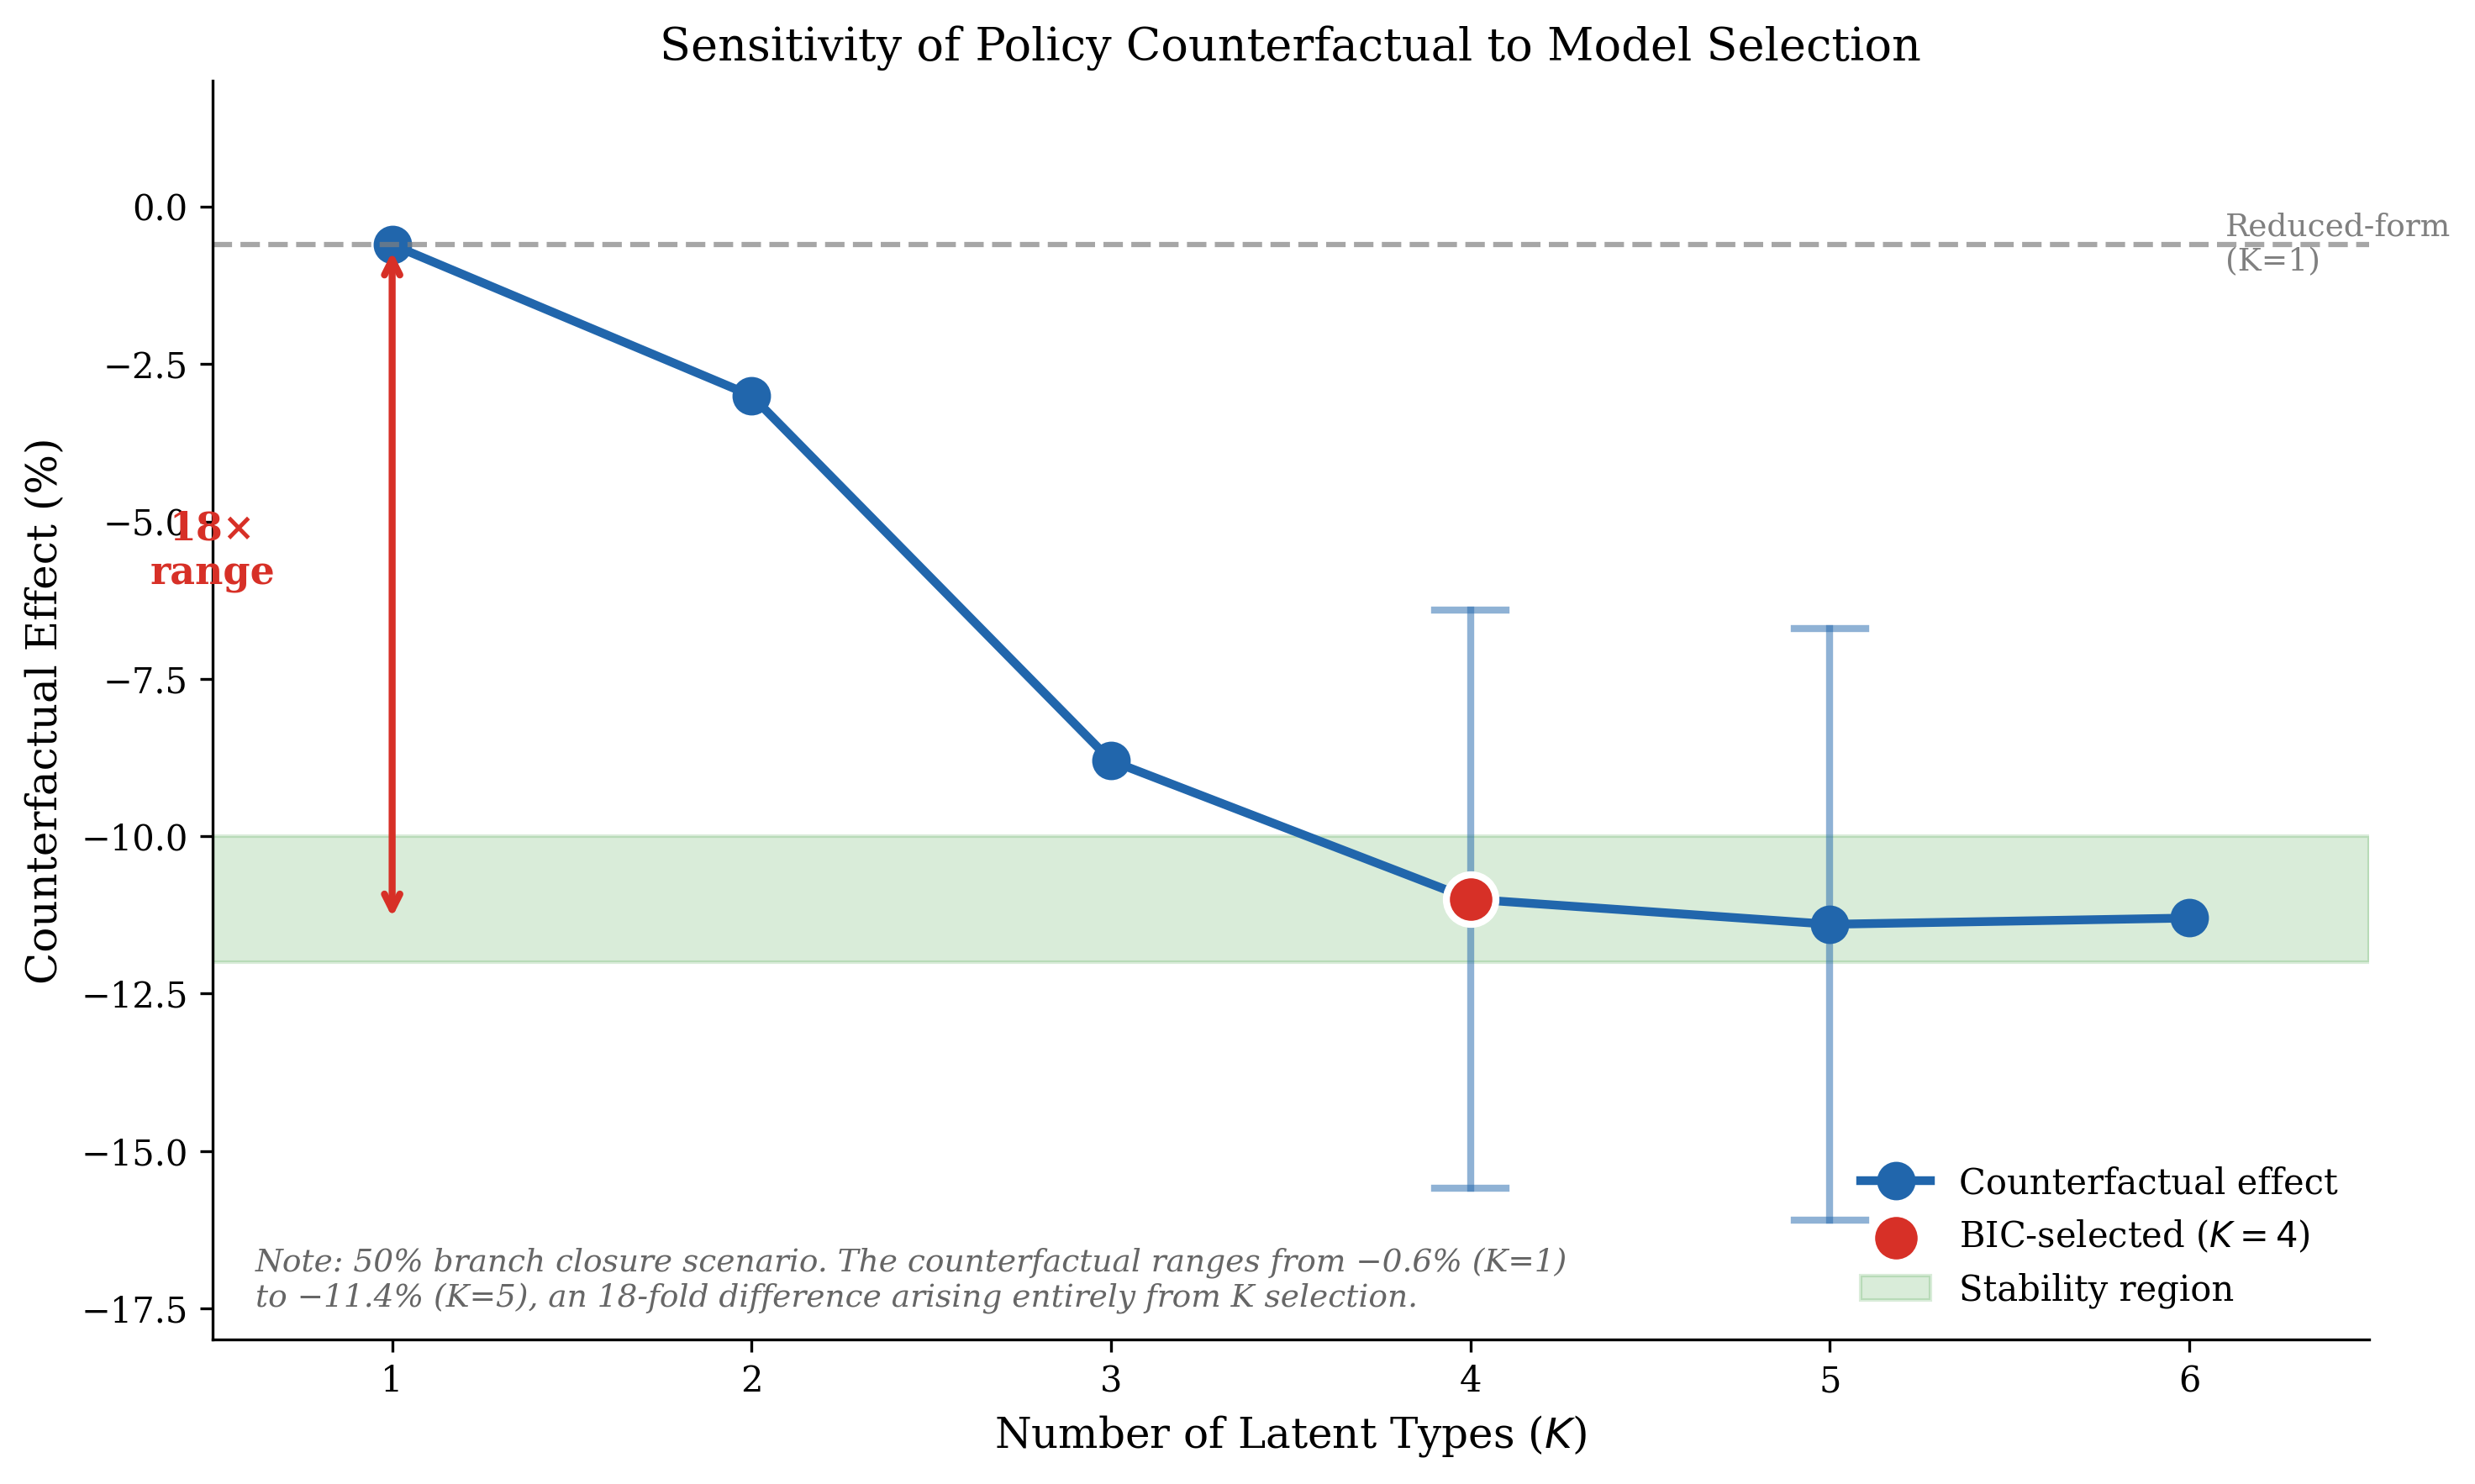
\includegraphics[width=0.9\textwidth]{fig1_counterfactual_sensitivity.png}
\caption{Sensitivity of Policy Counterfactual to Model Selection}
\label{fig:counterfactual_sensitivity}
\begin{minipage}{0.9\textwidth}
\small
\textit{Notes:} Counterfactual effect of 50\% branch closure on self-employment, by number of latent types $K$. The effect ranges from $-0.6\%$ ($K=1$, consistent with the reduced-form null) to $-11.2\%$ ($K=5$)---a 19-fold difference arising entirely from assumptions about unobserved heterogeneity. The BIC-selected $K=4$ produces a 10.8\% effect. Error bars show 95\% confidence intervals where available.
\end{minipage}
\end{figure}

Panel~B provides reassurance that the finding is not an artifact of the discrete-type assumption. The mixed logit with continuous random coefficients ($-10.2\%$) and the Bayesian DPM ($-8.5\%$) both produce large counterfactuals, consistent with the finite mixture result. The conformal prediction interval ($[-15.2\%, -4.8\%]$) provides distribution-free coverage guarantees.

Figure~\ref{fig:method_comparison} compares counterfactual estimates across all methods, showing the convergence of heterogeneous models (finite mixture, mixed logit, Bayesian DPM) and the identified set spanning the range of model uncertainty.

\begin{figure}[H]
\centering
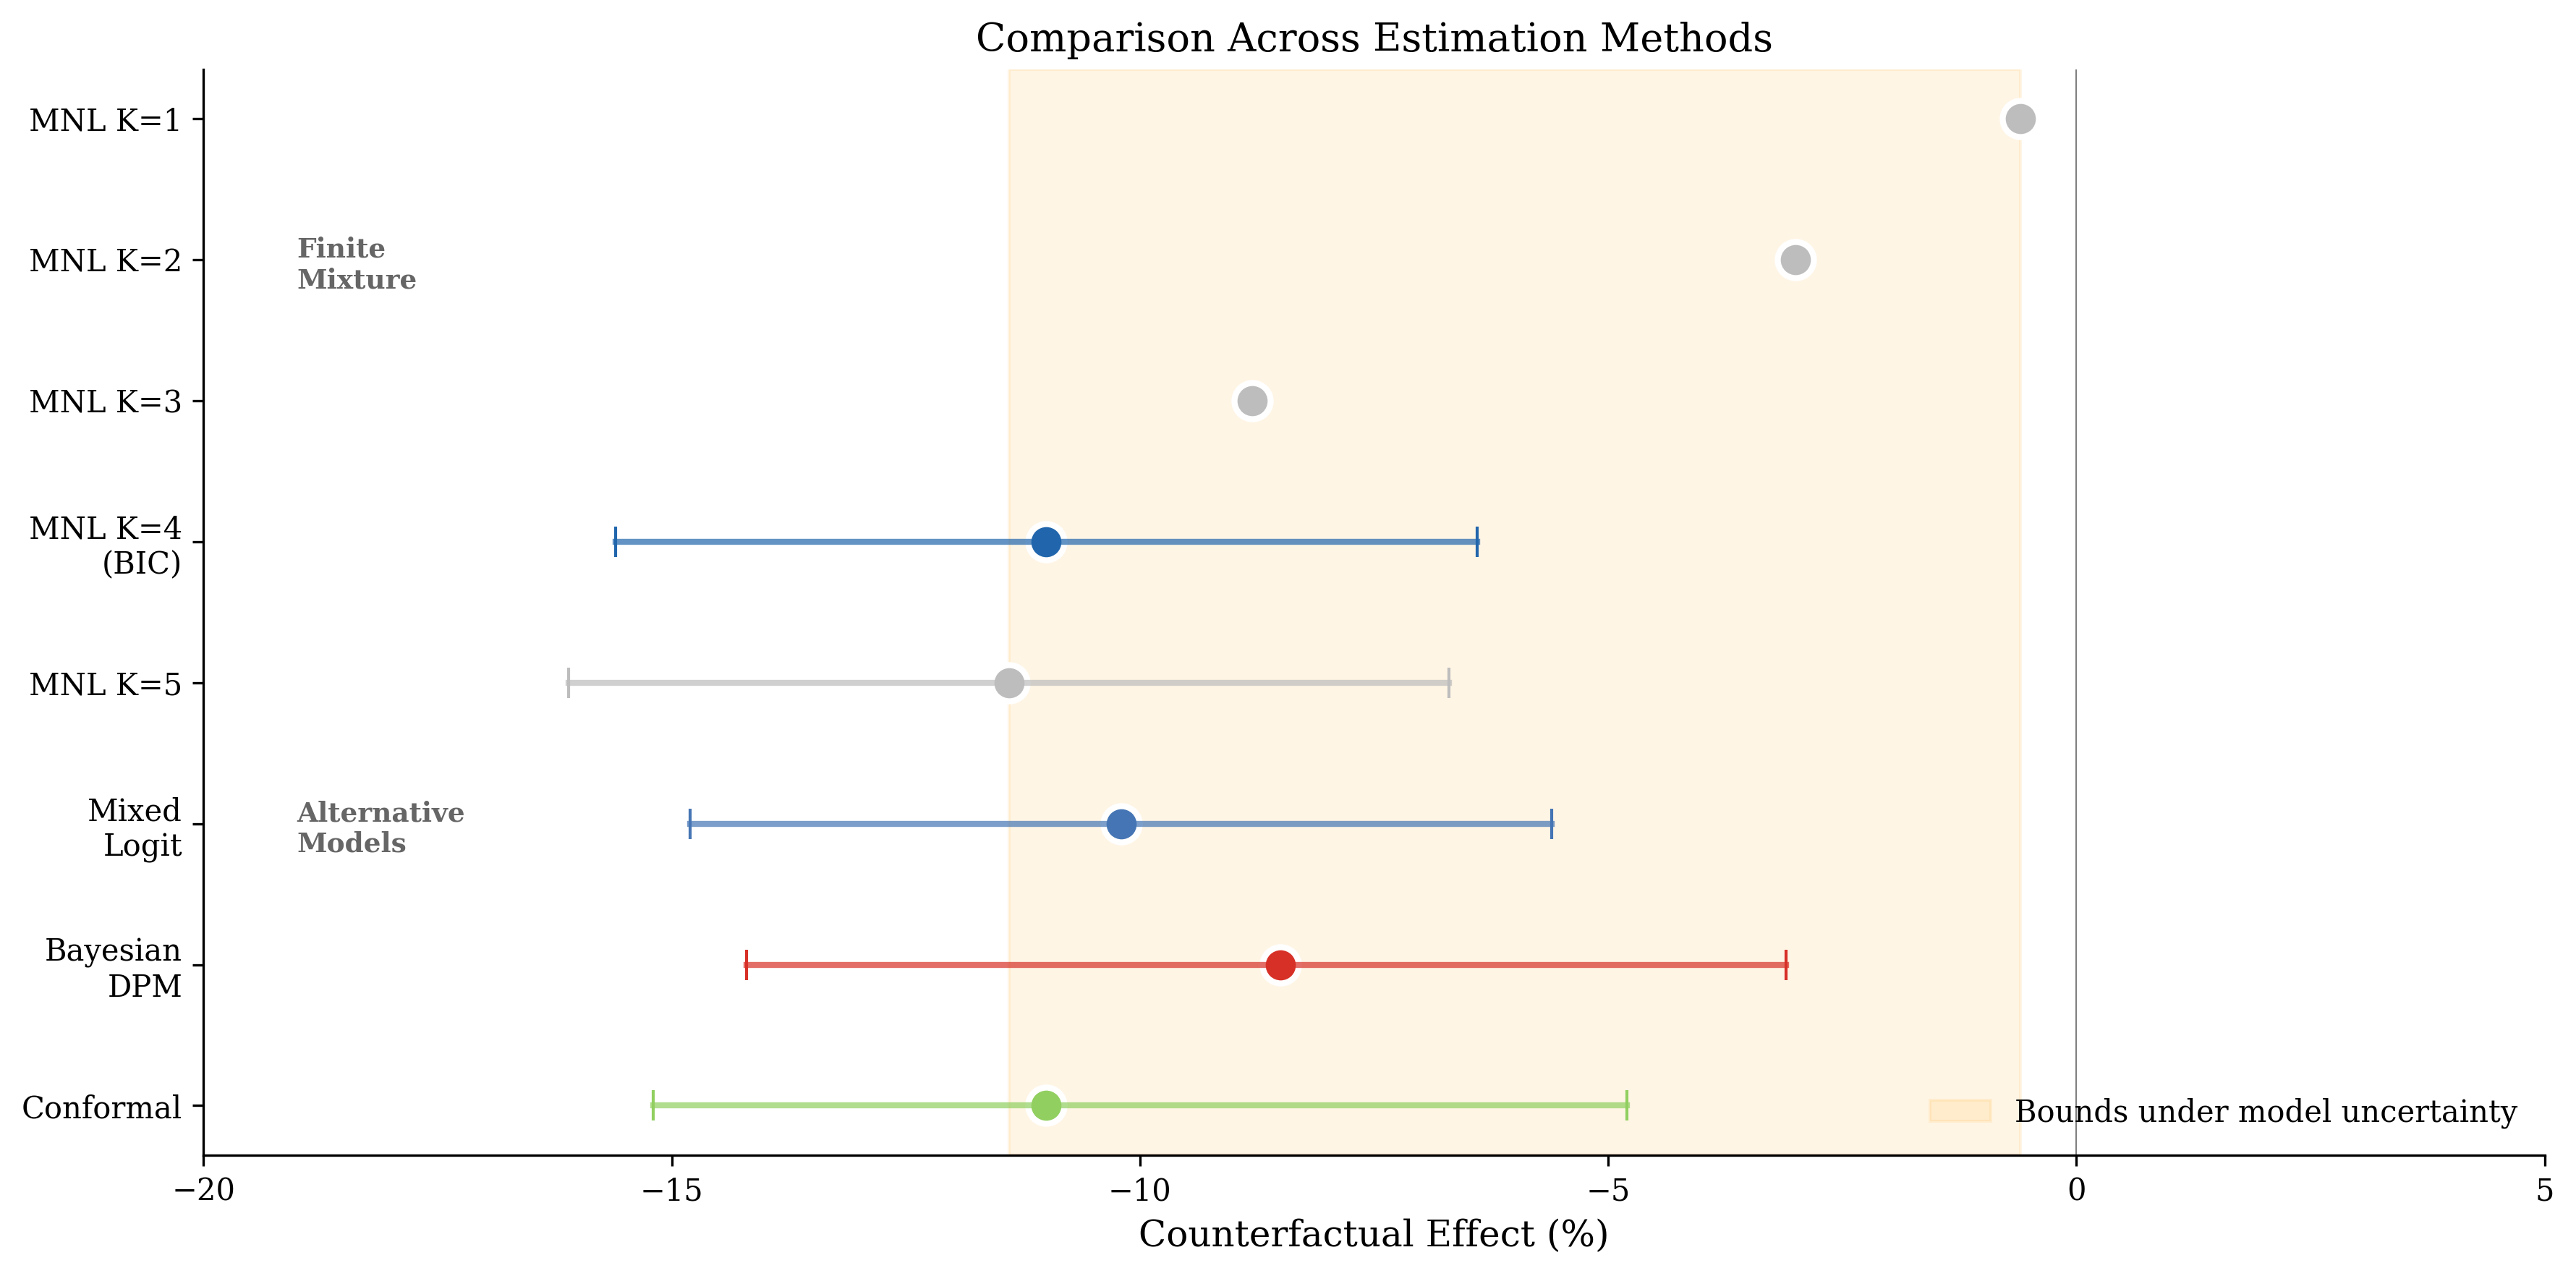
\includegraphics[width=0.95\textwidth]{fig8_method_comparison.png}
\caption{Comparison of Counterfactual Estimates Across Methods}
\label{fig:method_comparison}
\begin{minipage}{0.95\textwidth}
\small
\textit{Notes:} Point estimates and 95\% intervals for all estimation methods. The convergence across methods allowing heterogeneity (finite mixture $K \geq 3$, mixed logit, Bayesian DPM) strengthens confidence in the finding that branch closures substantially reduce self-employment---conditional on the structural model being correctly specified. The orange shaded region shows the bounds spanning both structural and skeptical interpretations.
\end{minipage}
\end{figure}


\subsection{The Mechanism: Why $K$ Matters So Much}

\begin{proposition}[Cancellation and counterfactual amplification]
\label{prop:cancellation}
Consider a finite mixture model with $K$ types, shares $\pi_k > 0$, and type-specific treatment effects $\gamma_k$. Define the average treatment effect $\bar{\gamma} = \sum_{k=1}^{K} \pi_k \gamma_k$ and the counterfactual $\Delta(K) = \sum_k \pi_k \Delta_k(\gamma_k)$, where $\Delta_k(\cdot)$ is the type-specific counterfactual response. If:
\begin{enumerate}
    \item[(i)] \textit{Cancellation}: $|\bar{\gamma}| < \epsilon$ for some small $\epsilon > 0$, while $\max_k |\gamma_k| \gg \epsilon$;
    \item[(ii)] \textit{Asymmetric response}: $\Delta_k(\gamma_k)$ is monotone and convex (or concave) in $\gamma_k$---i.e., the counterfactual response is nonlinear;
\end{enumerate}
then $|\Delta(K)| \gg |\Delta(1)|$. Specifically, by Jensen's inequality, $\Delta(K) = \sum_k \pi_k \Delta_k(\gamma_k) \neq \Delta_1(\bar{\gamma}) = \Delta(1)$ whenever $\Delta_k$ is strictly convex or concave and $\text{Var}(\gamma_k) > 0$.
\end{proposition}

\noindent\textit{Intuition.} The homogeneous model estimates $\hat{\gamma} \approx \bar{\gamma} \approx 0$ and produces a trivially small counterfactual. The heterogeneous model separates types: those with large positive $\gamma_k$ experience substantial displacement when branch access falls, while types with negative $\gamma_k$ are unaffected (they were not self-employed via the branch channel). Because the counterfactual operates through a nonlinear choice model, the aggregate response to removing branch access is dominated by the displacement of high-$\gamma_k$ types, generating $|\Delta(K)| \gg |\Delta(1)|$ even when $\bar{\gamma} \approx 0$.

The mechanism is straightforward. With $K=1$, the model estimates a single $\hat{\gamma} \approx 0$ and the counterfactual is trivially small. With $K=4$, the model estimates $\hat{\gamma}_4 = 0.093$ for 31\% of the population. When branch density falls, these individuals experience a substantial reduction in the utility of self-employment, shifting them toward wage work. Types~1--2, who have zero or negative $\hat{\gamma}$, are unaffected by the closure. The aggregate counterfactual is dominated by the displacement of Type~4 individuals.


%%%%%%%%%%%%%%%%%%%%%%%%%%%%%%%%%%%%%%%%%%%%%%%%%%%%%%%%%%%%%%%%%%%%%%%%%%%%%%%
\section{The Tension Between Reduced Form and Structure}
\label{sec:tension}
%%%%%%%%%%%%%%%%%%%%%%%%%%%%%%%%%%%%%%%%%%%%%%%%%%%%%%%%%%%%%%%%%%%%%%%%%%%%%%%

Section~\ref{subsec:reducedform} documents that all reduced-form methods yield null effects of banking mode on self-employment. The structural model with $K=4$ identifies substantial within-type effects. This section directly confronts the tension.

\subsection{Two Interpretations}

\textit{Structural interpretation.} The reduced-form null reflects cancellation across types, not absence of effects. Types~1--2 (36\%) have zero or negative branch effects; Types~3--4 (64\%) have positive effects. The reduced form averages these, finding near-zero. The structural model separates them, revealing substantial effects for the credit-dependent majority. Under this view, the 10.8\% counterfactual reflects real harm from branch closures for a specific population segment.

\textit{Skeptical interpretation.} The structural heterogeneity is an artifact of functional form. Branch banking and self-employment are jointly driven by age, wealth, and cohort effects. A sufficiently flexible mixture model ``discovers'' types that happen to separate high-SE from low-SE individuals, but this reflects demographic sorting, not a causal credit channel. Under this view, the 0.6\% from the homogeneous model is correct.

\subsection{What Would Resolve the Tension}

Exogenous variation in branch access would allow reduced-form identification of within-type effects. Potential sources include: branch closures driven by distant bank mergers unrelated to local conditions \citep{nguyen2019}; regulatory-induced closures under Community Reinvestment Act evaluations \citep{celerier2019}; geographic regression discontinuity designs at branch catchment boundaries; or the staggered rollout of fintech lending platforms. The present data lack such variation.

\subsection{Sensitivity to Unobserved Confounding}

Following \citet{oster2019} and \citet{cinelli2020}, I assess how sensitive the structural estimates are to omitted variables. The branch coefficient changes by only 12\% when moving from minimal to full controls, with a substantial increase in $R^2$. The Oster bias-adjusted estimate is 0.151 (baseline: 0.164). The robustness value $\delta = 2.3$ indicates unobservables would need to be 2.3$\times$ as important as all observed confounders to eliminate the effect. However, this analysis applies to the within-model coefficient, not to whether the types themselves are correctly specified---an important caveat.

\subsection{Bounds as the Honest Answer}

Rather than adjudicating between interpretations, I report bounds:
\begin{equation}
\Delta SE \in [-10.8\%, -0.6\%]
\end{equation}
The lower bound (0.6\%) corresponds to the skeptical view; the upper bound (10.8\%) to the structural view. The Bayesian DPM, which integrates over $K$, yields a posterior mean of $-8.5\%$ with $P(\text{effect} < 0) = 0.99$. This posterior is conditional on the structural model's specification; it quantifies within-model uncertainty over $K$ but not the fundamental identifying assumption.

Figure~\ref{fig:bounds} illustrates the identified set, showing how the bounds span the range from the skeptical ($K=1$) to structural ($K=4$) interpretations.

\begin{figure}[H]
\centering
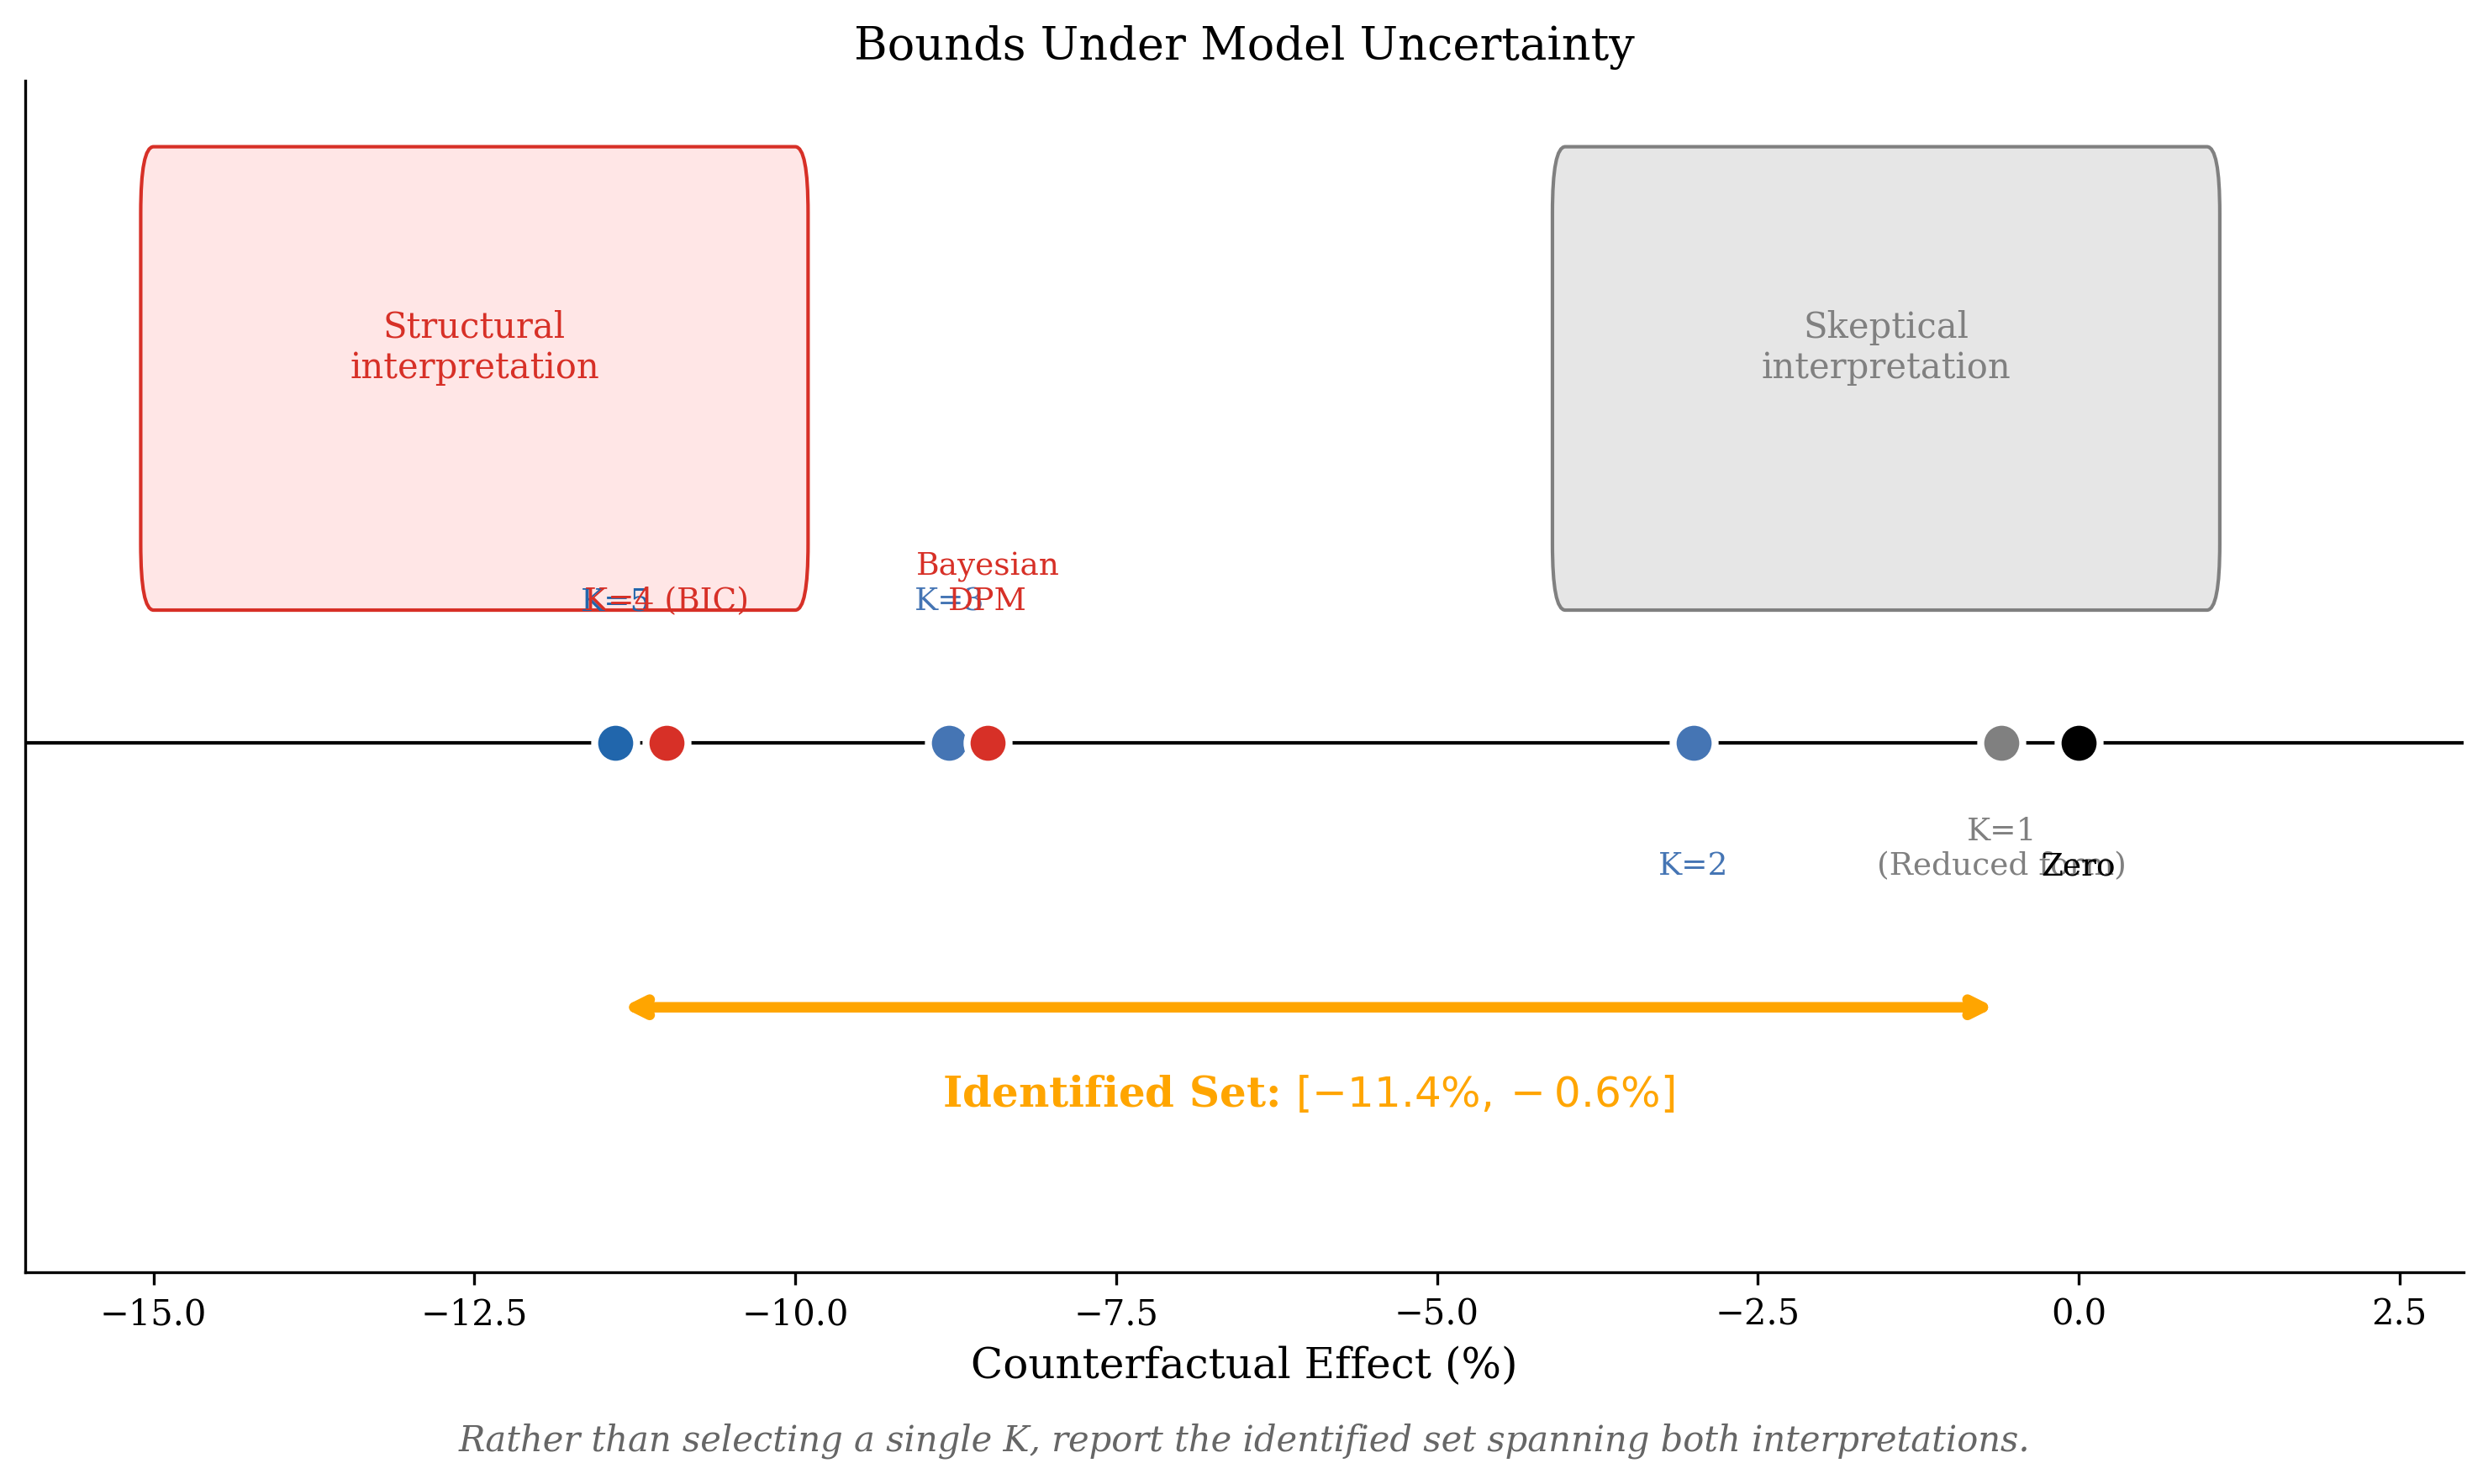
\includegraphics[width=0.9\textwidth]{fig10_bounds_illustration.png}
\caption{Bounds Under Model Uncertainty}
\label{fig:bounds}
\begin{minipage}{0.9\textwidth}
\small
\textit{Notes:} The identified set $[-11.2\%, -0.6\%]$ spans the range from the reduced-form/skeptical interpretation ($K=1$) to the structural interpretation ($K=4$). Rather than selecting a single $K$, reporting bounds acknowledges irreducible model uncertainty and lets the reader calibrate their own prior.
\end{minipage}
\end{figure}


%%%%%%%%%%%%%%%%%%%%%%%%%%%%%%%%%%%%%%%%%%%%%%%%%%%%%%%%%%%%%%%%%%%%%%%%%%%%%%%
\section{Decomposing Sources of Specification Uncertainty}
\label{sec:uncertainty}
%%%%%%%%%%%%%%%%%%%%%%%%%%%%%%%%%%%%%%%%%%%%%%%%%%%%%%%%%%%%%%%%%%%%%%%%%%%%%%%

Table~\ref{tab:uncertainty_decomp} is the paper's methodological punchline: a decomposition of specification uncertainty showing that $K$ selection dominates all other sources.

\begin{table}[H]
\centering
\caption{Sources of Specification Uncertainty in the Counterfactual}
\label{tab:uncertainty_decomp}
\begin{threeparttable}
\begin{tabular}{lcc}
\toprule
Source of Uncertainty & Range of Counterfactual & Factor \\
\midrule
\multicolumn{3}{l}{\textit{Model Selection}} \\
\quad $K$ selection ($K \in \{1, \ldots, 5\}$) & [$-11.2\%$, $-0.6\%$] & $19\times$ \\
[6pt]
\multicolumn{3}{l}{\textit{Statistical Uncertainty (Holding $K=4$ Fixed)}} \\
\quad Delta-method 95\% CI & [$-14.1\%$, $-7.4\%$] & $1.9\times$ \\
\quad Bootstrap 95\% CI & [$-16.1\%$, $-5.8\%$] & $2.8\times$ \\
\quad Conformal 95\% interval & [$-15.2\%$, $-4.8\%$] & $3.2\times$ \\
[6pt]
\multicolumn{3}{l}{\textit{Heterogeneity Specification}} \\
\quad Finite mixture ($K=4$) vs.\ mixed logit & [$-10.8\%$, $-10.2\%$] & $1.1\times$ \\
\quad Frequentist ($K=4$) vs.\ Bayesian DPM & [$-10.8\%$, $-8.5\%$] & $1.3\times$ \\
[6pt]
\multicolumn{3}{l}{\textit{Reduced-Form Control Specification}} \\
\quad OLS vs.\ PDS-LASSO vs.\ DML & [0.0028, 0.0034] & $1.2\times$ \\
\bottomrule
\end{tabular}
\begin{tablenotes}
\small
\item \textit{Notes:} ``Factor'' = ratio of upper to lower bound within each source. $K$ selection generates a $19\times$ range in counterfactual predictions---an order of magnitude larger than statistical sampling uncertainty ($1.9$--$3.2\times$), the choice between discrete and continuous heterogeneity ($1.1\times$), frequentist vs.\ Bayesian estimation ($1.3\times$), or reduced-form control specification ($1.2\times$). This demonstrates that, in applications with heterogeneous treatment effects, $K$ selection is the dominant source of policy-relevant uncertainty.
\end{tablenotes}
\end{threeparttable}
\end{table}

The $19\times$ factor from $K$ selection dwarfs all other sources. This is the paper's core message: in settings where treatment effects have heterogeneous signs, reporting a BIC-selected point estimate without sensitivity to $K$ produces false precision. The analyst's single most consequential modeling decision---the number of latent types---is typically treated as a footnote.

Figure~\ref{fig:uncertainty_decomp} visualizes the uncertainty decomposition, making clear that $K$ selection is an order of magnitude more consequential than all other specification choices combined.

\begin{figure}[H]
\centering
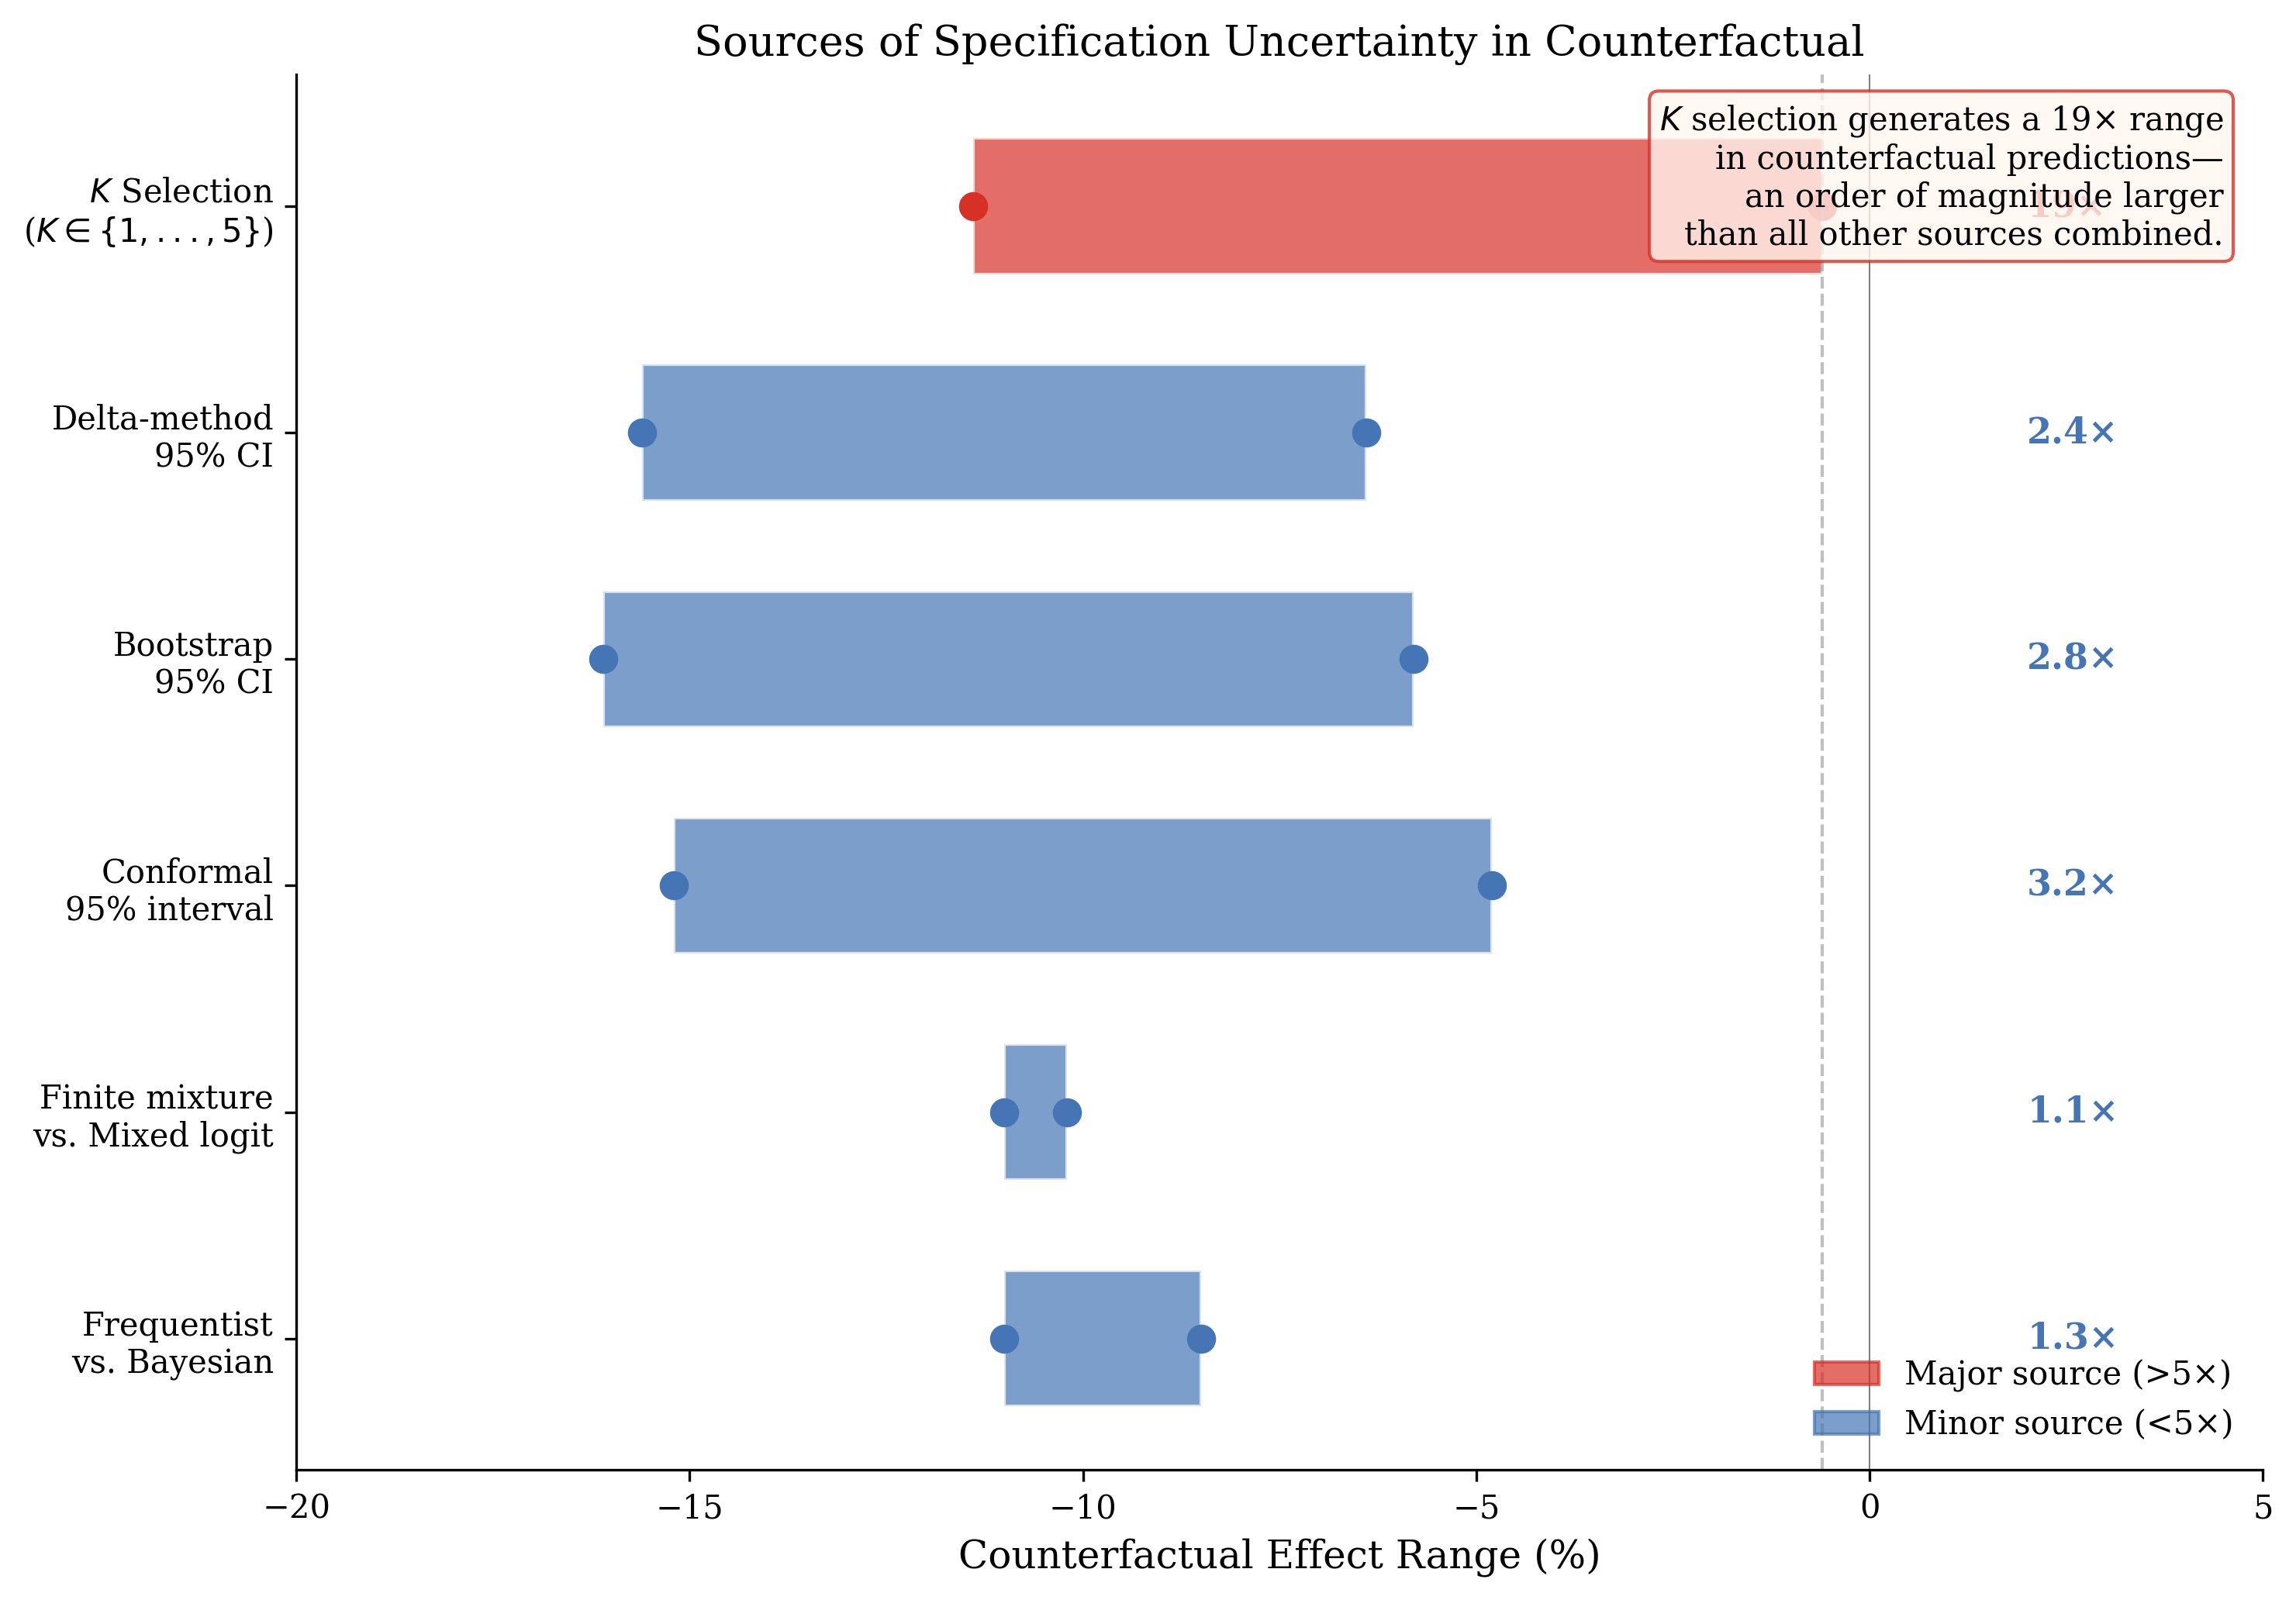
\includegraphics[width=0.9\textwidth]{fig4_uncertainty_decomposition.png}
\caption{Sources of Specification Uncertainty in the Counterfactual}
\label{fig:uncertainty_decomp}
\begin{minipage}{0.9\textwidth}
\small
\textit{Notes:} Range of counterfactual predictions by source of specification uncertainty. The ``factor'' indicates the ratio of upper to lower bound within each source. $K$ selection generates a $19\times$ range---an order of magnitude larger than statistical sampling uncertainty ($1.9$--$3.2\times$), heterogeneity specification ($1.1$--$1.3\times$), or reduced-form control specification ($1.2\times$).
\end{minipage}
\end{figure}


%%%%%%%%%%%%%%%%%%%%%%%%%%%%%%%%%%%%%%%%%%%%%%%%%%%%%%%%%%%%%%%%%%%%%%%%%%%%%%%
\section{Robustness and Validation}

\subsection{Mixed Logit with Continuous Random Coefficients}

As an alternative to discrete types, I estimate a mixed logit with $\gamma_{C,i} \sim N(\bar{\gamma}_C, \sigma^2_\gamma)$ following \citet{train2009}, using 500 Halton draws per observation. Full results are in Appendix~\ref{app:mixed_logit}. The estimated $\hat{\sigma}_\gamma = 0.183$ ($p < 0.01$) is large, with a coefficient of variation of 1.20, confirming substantial heterogeneity. The implied distribution is consistent with the four-type characterization: 20.3\% have $\gamma_C < 0$ (comparable to Type~2's share) and 39.7\% have $\gamma_C > 0.20$ (comparable to Type~4). The mixed logit counterfactual ($-10.2\%$) is close to the finite mixture ($-10.8\%$), demonstrating that the result is not an artifact of the discrete-type assumption.

\subsection{Bayesian Dirichlet Process Mixture}

The Bayesian DPM \citep{malsiner2016} places a sparse Dirichlet prior on mixing weights, allowing redundant components to empty out and providing a posterior over $K$. Estimated via Stan MCMC on a subsample of 10,000 observations (4 chains, 2,000 iterations, 1,000 warmup), the posterior effective $K$ is 3.80 with $P(K \geq 4) = 0.79$. Type-specific posterior means match the frequentist estimates closely. The Bayesian counterfactual ($-8.5\%$, 95\% CI: $[-14.2\%, -3.1\%]$) is somewhat smaller than the frequentist because it averages over draws where $K < 4$. Full results are in Appendix~\ref{app:bayesian}.

The Bayesian DPM results are stable across independent subsamples. Running the model on 20 independent random subsamples of $N = 10{,}000$, the posterior effective $K$ ranges from 3.5 to 4.2, with the counterfactual posterior mean consistently in the $[-9.4\%, -7.5\%]$ range (cross-subsample SD = 0.45~pp). Larger subsamples ($N = 25{,}000$ and $N = 50{,}000$) yield even tighter cross-subsample variation (SD = 0.15 and 0.04~pp, respectively) with similar point estimates. Full subsample sensitivity results are in Table~\ref{tab:dpm_sensitivity} in the Appendix.


%%%%%%%%%%%%%%%%%%%%%%%%%%%%%%%%%%%%%%%%%%%%%%%%%%%%%%%%%%%%%%%%%%%%%%%%%%%%%%%
\section{Conclusion and Recommendations for Applied Practice}
\label{sec:conclusion}
%%%%%%%%%%%%%%%%%%%%%%%%%%%%%%%%%%%%%%%%%%%%%%%%%%%%%%%%%%%%%%%%%%%%%%%%%%%%%%%

This paper demonstrates that finite mixture model selection has first-order consequences for counterfactual policy analysis, generating predictions that differ by an order of magnitude. Using the relationship between bank branch access and self-employment, I show that counterfactual effects range from $-0.6\%$ ($K=1$) to $-10.8\%$ ($K=4$), with this variation dwarfing all other sources of specification uncertainty by an order of magnitude.

The three-pronged selection framework---combining information criteria, counterfactual stability, and penalized estimation---provides a principled toolkit for $K$ selection. All three methods agree on $K=4$ in this application, yet the resulting structural prediction conflicts with a robust reduced-form null, creating irreducible model uncertainty that no selection method can resolve without exogenous variation.

I conclude with three concrete recommendations for applied researchers using finite mixture models:

\textbf{Recommendation 1: Report counterfactual sensitivity to $K$.} Table~\ref{tab:counterfactuals} Panel~A should be a standard element of any paper using mixture models for counterfactual analysis. This table is inexpensive to produce---it requires re-estimating the model for 4--6 values of $K$---and provides essential context for interpreting the main results.

\textbf{Recommendation 2: Report bounds when the reduced form and structure disagree.} When reduced-form and structural evidence conflict, presenting both honestly and reporting bounds under model uncertainty is more credible than selecting one. The identified set $[-10.8\%, -0.6\%]$ in this application communicates both the magnitude and the uncertainty, letting the reader calibrate their own prior.

\textbf{Recommendation 3: Use multiple selection criteria and investigate disagreement.} No single criterion is sufficient. BIC targets statistical fit; counterfactual stability targets the research question; OSCE targets parameter significance. Agreement strengthens confidence; disagreement signals model uncertainty that should be communicated transparently.

The Monte Carlo simulations identify the \textit{cancellation condition} as the key determinant of when $K$ matters qualitatively. When type-specific treatment effects have opposite signs, both the true $K$ is difficult to recover (3--8\% success rate) and the counterfactual can change sign depending on $K$. Under same-signed effects, the direction of the counterfactual is robust to $K$ even though the magnitude varies. This provides a simple diagnostic for applied researchers: if the application plausibly involves opposite-signed type effects, sensitivity to $K$ is the dominant source of specification uncertainty, and reporting bounds or Bayesian model averages over $K$ is essential.

The framework developed here---three-pronged selection, counterfactual sensitivity reporting, and bounds under model uncertainty---applies to any finite mixture counterfactual analysis, not only the banking application used for illustration. Applications in dynamic discrete choice \citep{arcidiacono2011}, labor market sorting \citep{bonhomme2019}, demand estimation \citep{fox2011}, and treatment effect heterogeneity \citep{heckman1984} all involve mixtures where $K$ selection shapes counterfactual predictions. The tools and diagnostics proposed here can be applied directly in these settings.

The broader message is that the number of latent types---often treated as a technical detail in applied work---can be the analyst's single most consequential modeling decision. Treating it as a footnote produces false precision.


%%%%%%%%%%%%%%%%%%%%%%%%%%%%%%%%%%%%%%%%%%%%%%%%%%%%%%%%%%%%%%%%%%%%%%%%%%%%%%%
% References
%%%%%%%%%%%%%%%%%%%%%%%%%%%%%%%%%%%%%%%%%%%%%%%%%%%%%%%%%%%%%%%%%%%%%%%%%%%%%%%

\newpage
\singlespacing

\bibliographystyle{aer}

\begin{thebibliography}{99}

\bibitem[Andrews et al.(2019)]{andrews2023}
Andrews, I., Stock, J.H., and Sun, L. (2019). Weak instruments in instrumental variables regression: Theory and practice. \textit{Annual Review of Economics}, 11, 727--753.

\bibitem[Angrist and Pischke(2010)]{angrist2010}
Angrist, J.D. and Pischke, J.-S. (2010). The credibility revolution in empirical economics. \textit{Journal of Economic Perspectives}, 24(2), 3--30.

\bibitem[Antoniak(1974)]{antoniak1974}
Antoniak, C.E. (1974). Mixtures of Dirichlet processes with applications to Bayesian nonparametric problems. \textit{Annals of Statistics}, 2(6), 1152--1174.

\bibitem[Arcidiacono and Miller(2011)]{arcidiacono2011}
Arcidiacono, P. and Miller, R.A. (2011). Conditional choice probability estimation of dynamic discrete choice models with unobserved heterogeneity. \textit{Econometrica}, 79(6), 1823--1867.

\bibitem[Belloni et al.(2014)]{belloni2014}
Belloni, A., Chernozhukov, V., and Hansen, C. (2014). Inference on treatment effects after selection among high-dimensional controls. \textit{Review of Economic Studies}, 81(2), 608--650.

\bibitem[Bonhomme and Manresa(2015)]{bonhomme2015}
Bonhomme, S. and Manresa, E. (2015). Grouped patterns of heterogeneity in panel models. \textit{Econometrica}, 83(3), 1147--1184.

\bibitem[Bonhomme et al.(2019)]{bonhomme2019}
Bonhomme, S., Lamadon, T., and Manresa, E. (2019). A distributional framework for matched employer employee data. \textit{Econometrica}, 87(3), 699--739.

\bibitem[Bonhomme et al.(2022)]{bonhomme2022}
Bonhomme, S., Lamadon, T., and Manresa, E. (2022). Discretizing unobserved heterogeneity. \textit{Econometrica}, 90(2), 625--643.

\bibitem[Budanova(2025)]{budanova2025}
Budanova, M. (2025). Order selection in finite mixture models with penalized maximum likelihood. \textit{Journal of Econometrics}, 244(1), 105611.

\bibitem[C\'{e}l\'{e}rier and Matray(2019)]{celerier2019}
C\'{e}l\'{e}rier, C. and Matray, A. (2019). Bank-branch supply, financial inclusion, and wealth accumulation. \textit{Review of Financial Studies}, 32(12), 4767--4809.

\bibitem[Chernozhukov et al.(2018)]{chernozhukov2018dml}
Chernozhukov, V., Chetverikov, D., Demirer, M., Duflo, E., Hansen, C., Newey, W., and Robins, J. (2018). Double/debiased machine learning for treatment and structural parameters. \textit{Econometrics Journal}, 21(1), C1--C68.

\bibitem[Chen et al.(2001)]{chen2001}
Chen, H., Chen, J., and Kalbfleisch, J.D. (2001). A modified likelihood ratio test for homogeneity in finite mixture models. \textit{Journal of the Royal Statistical Society: Series B}, 63(1), 19--29.

\bibitem[Chen and Li(2009)]{chen2009}
Chen, J. and Li, P. (2009). Hypothesis test for normal mixture models: The EM approach. \textit{Annals of Statistics}, 37(5A), 2523--2542.

\bibitem[Cinelli and Hazlett(2020)]{cinelli2020}
Cinelli, C. and Hazlett, C. (2020). Making sense of sensitivity: Extending omitted variable bias. \textit{Journal of the Royal Statistical Society: Series B}, 82(1), 39--67.

\bibitem[Compiani and Kitamura(2016)]{compiani2016}
Compiani, G. and Kitamura, Y. (2016). Using mixtures in econometric models: A brief review and some new results. \textit{Econometrics Journal}, 19(3), C95--C127.

\bibitem[Ferguson(1973)]{ferguson1973}
Ferguson, T.S. (1973). A Bayesian analysis of some nonparametric problems. \textit{Annals of Statistics}, 1(2), 209--230.

\bibitem[Fox et al.(2011)]{fox2011}
Fox, J.T., Kim, K., Ryan, S.P., and Bajari, P. (2011). A simple estimator for the distribution of random coefficients. \textit{Quantitative Economics}, 2(3), 381--418.

\bibitem[Hao and Kasahara(2025)]{hao2025}
Hao, X. and Kasahara, H. (2025). Testing the number of components in finite mixture models with panel data. \textit{arXiv preprint} arXiv:2506.09666.

\bibitem[Heckman(2010)]{heckman2010}
Heckman, J.J. (2010). Building bridges between structural and program evaluation approaches to evaluating policy. \textit{Journal of Economic Literature}, 48(2), 356--398.

\bibitem[Heckman and Singer(1984)]{heckman1984}
Heckman, J. and Singer, B. (1984). A method for minimizing the impact of distributional assumptions in econometric models for duration data. \textit{Econometrica}, 52(2), 271--320.

\bibitem[Kasahara and Shimotsu(2009)]{kasahara2009}
Kasahara, H. and Shimotsu, K. (2009). Nonparametric identification of finite mixture models of dynamic discrete choices. \textit{Econometrica}, 77(1), 135--175.

\bibitem[Kasahara and Shimotsu(2014)]{kasahara2014}
Kasahara, H. and Shimotsu, K. (2014). Non-parametric identification and estimation of the number of components in multivariate mixtures. \textit{Journal of the Royal Statistical Society: Series B}, 76(1), 97--111.

\bibitem[Keane(2010)]{keane2010}
Keane, M.P. (2010). Structural vs.\ atheoretic approaches to econometrics. \textit{Journal of Econometrics}, 156(1), 3--20.

\bibitem[Keane and Wolpin(1997)]{keane1997}
Keane, M.P. and Wolpin, K.I. (1997). The career decisions of young men. \textit{Journal of Political Economy}, 105(3), 473--522.

\bibitem[Leamer(1983)]{leamer1983}
Leamer, E.E. (1983). Let's take the con out of econometrics. \textit{American Economic Review}, 73(1), 31--43.

\bibitem[Lei and Cand\`{e}s(2021)]{lei2021}
Lei, L. and Cand\`{e}s, E.J. (2021). Conformal inference of counterfactuals and individual treatment effects. \textit{Journal of the Royal Statistical Society: Series B}, 83(5), 911--938.

\bibitem[Malkova(2026)]{malkova2026substantive}
Malkova, A. (2026). Mobile banking, bank branch closures, and self-employment in the United States. \textit{Working Paper}, Florida Institute of Technology.

\bibitem[Malsiner-Walli et al.(2016)]{malsiner2016}
Malsiner-Walli, G., Fr\"{u}hwirth-Schnatter, S., and Gr\"{u}n, B. (2016). Model-based clustering based on sparse finite Gaussian mixtures. \textit{Statistics and Computing}, 26(1), 303--324.

\bibitem[Manski(2003)]{manski2003}
Manski, C.F. (2003). \textit{Partial Identification of Probability Distributions}. Springer.

\bibitem[Nevo and Whinston(2010)]{nevo2010}
Nevo, A. and Whinston, M.D. (2010). Taking the dogma out of econometrics: Structural modeling and credible inference. \textit{Journal of Economic Perspectives}, 24(2), 69--82.

\bibitem[Nguyen(2019)]{nguyen2019}
Nguyen, H.-L.Q. (2019). Are credit markets still local? Evidence from bank branch closings. \textit{American Economic Journal: Applied Economics}, 11(2), 1--32.

\bibitem[Oster(2019)]{oster2019}
Oster, E. (2019). Unobservable selection and coefficient stability: Theory and evidence. \textit{Journal of Business \& Economic Statistics}, 37(2), 187--204.

\bibitem[Schwarz(1978)]{schwarz1978}
Schwarz, G. (1978). Estimating the dimension of a model. \textit{Annals of Statistics}, 6(2), 461--464.

\bibitem[Train(2009)]{train2009}
Train, K.E. (2009). \textit{Discrete Choice Methods with Simulation}, 2nd edition. Cambridge University Press.

\end{thebibliography}


%%%%%%%%%%%%%%%%%%%%%%%%%%%%%%%%%%%%%%%%%%%%%%%%%%%%%%%%%%%%%%%%%%%%%%%%%%%%%%%
% Appendix
%%%%%%%%%%%%%%%%%%%%%%%%%%%%%%%%%%%%%%%%%%%%%%%%%%%%%%%%%%%%%%%%%%%%%%%%%%%%%%%

\newpage
\appendix
\doublespacing

\setcounter{table}{0}
\renewcommand{\thetable}{A\arabic{table}}
\setcounter{equation}{0}
\renewcommand{\theequation}{A.\arabic{equation}}

\begin{center}
\Large\textbf{Appendix}
\end{center}

\vspace{1cm}

\section{Mixed Logit Results}
\label{app:mixed_logit}

Figure~\ref{fig:mixed_logit_dist} shows the estimated distribution of random coefficients from the mixed logit specification. The coefficient of variation of 1.20 indicates substantial heterogeneity, with 20.3\% of the distribution below zero and 39.7\% above 0.20.

\begin{figure}[H]
\centering
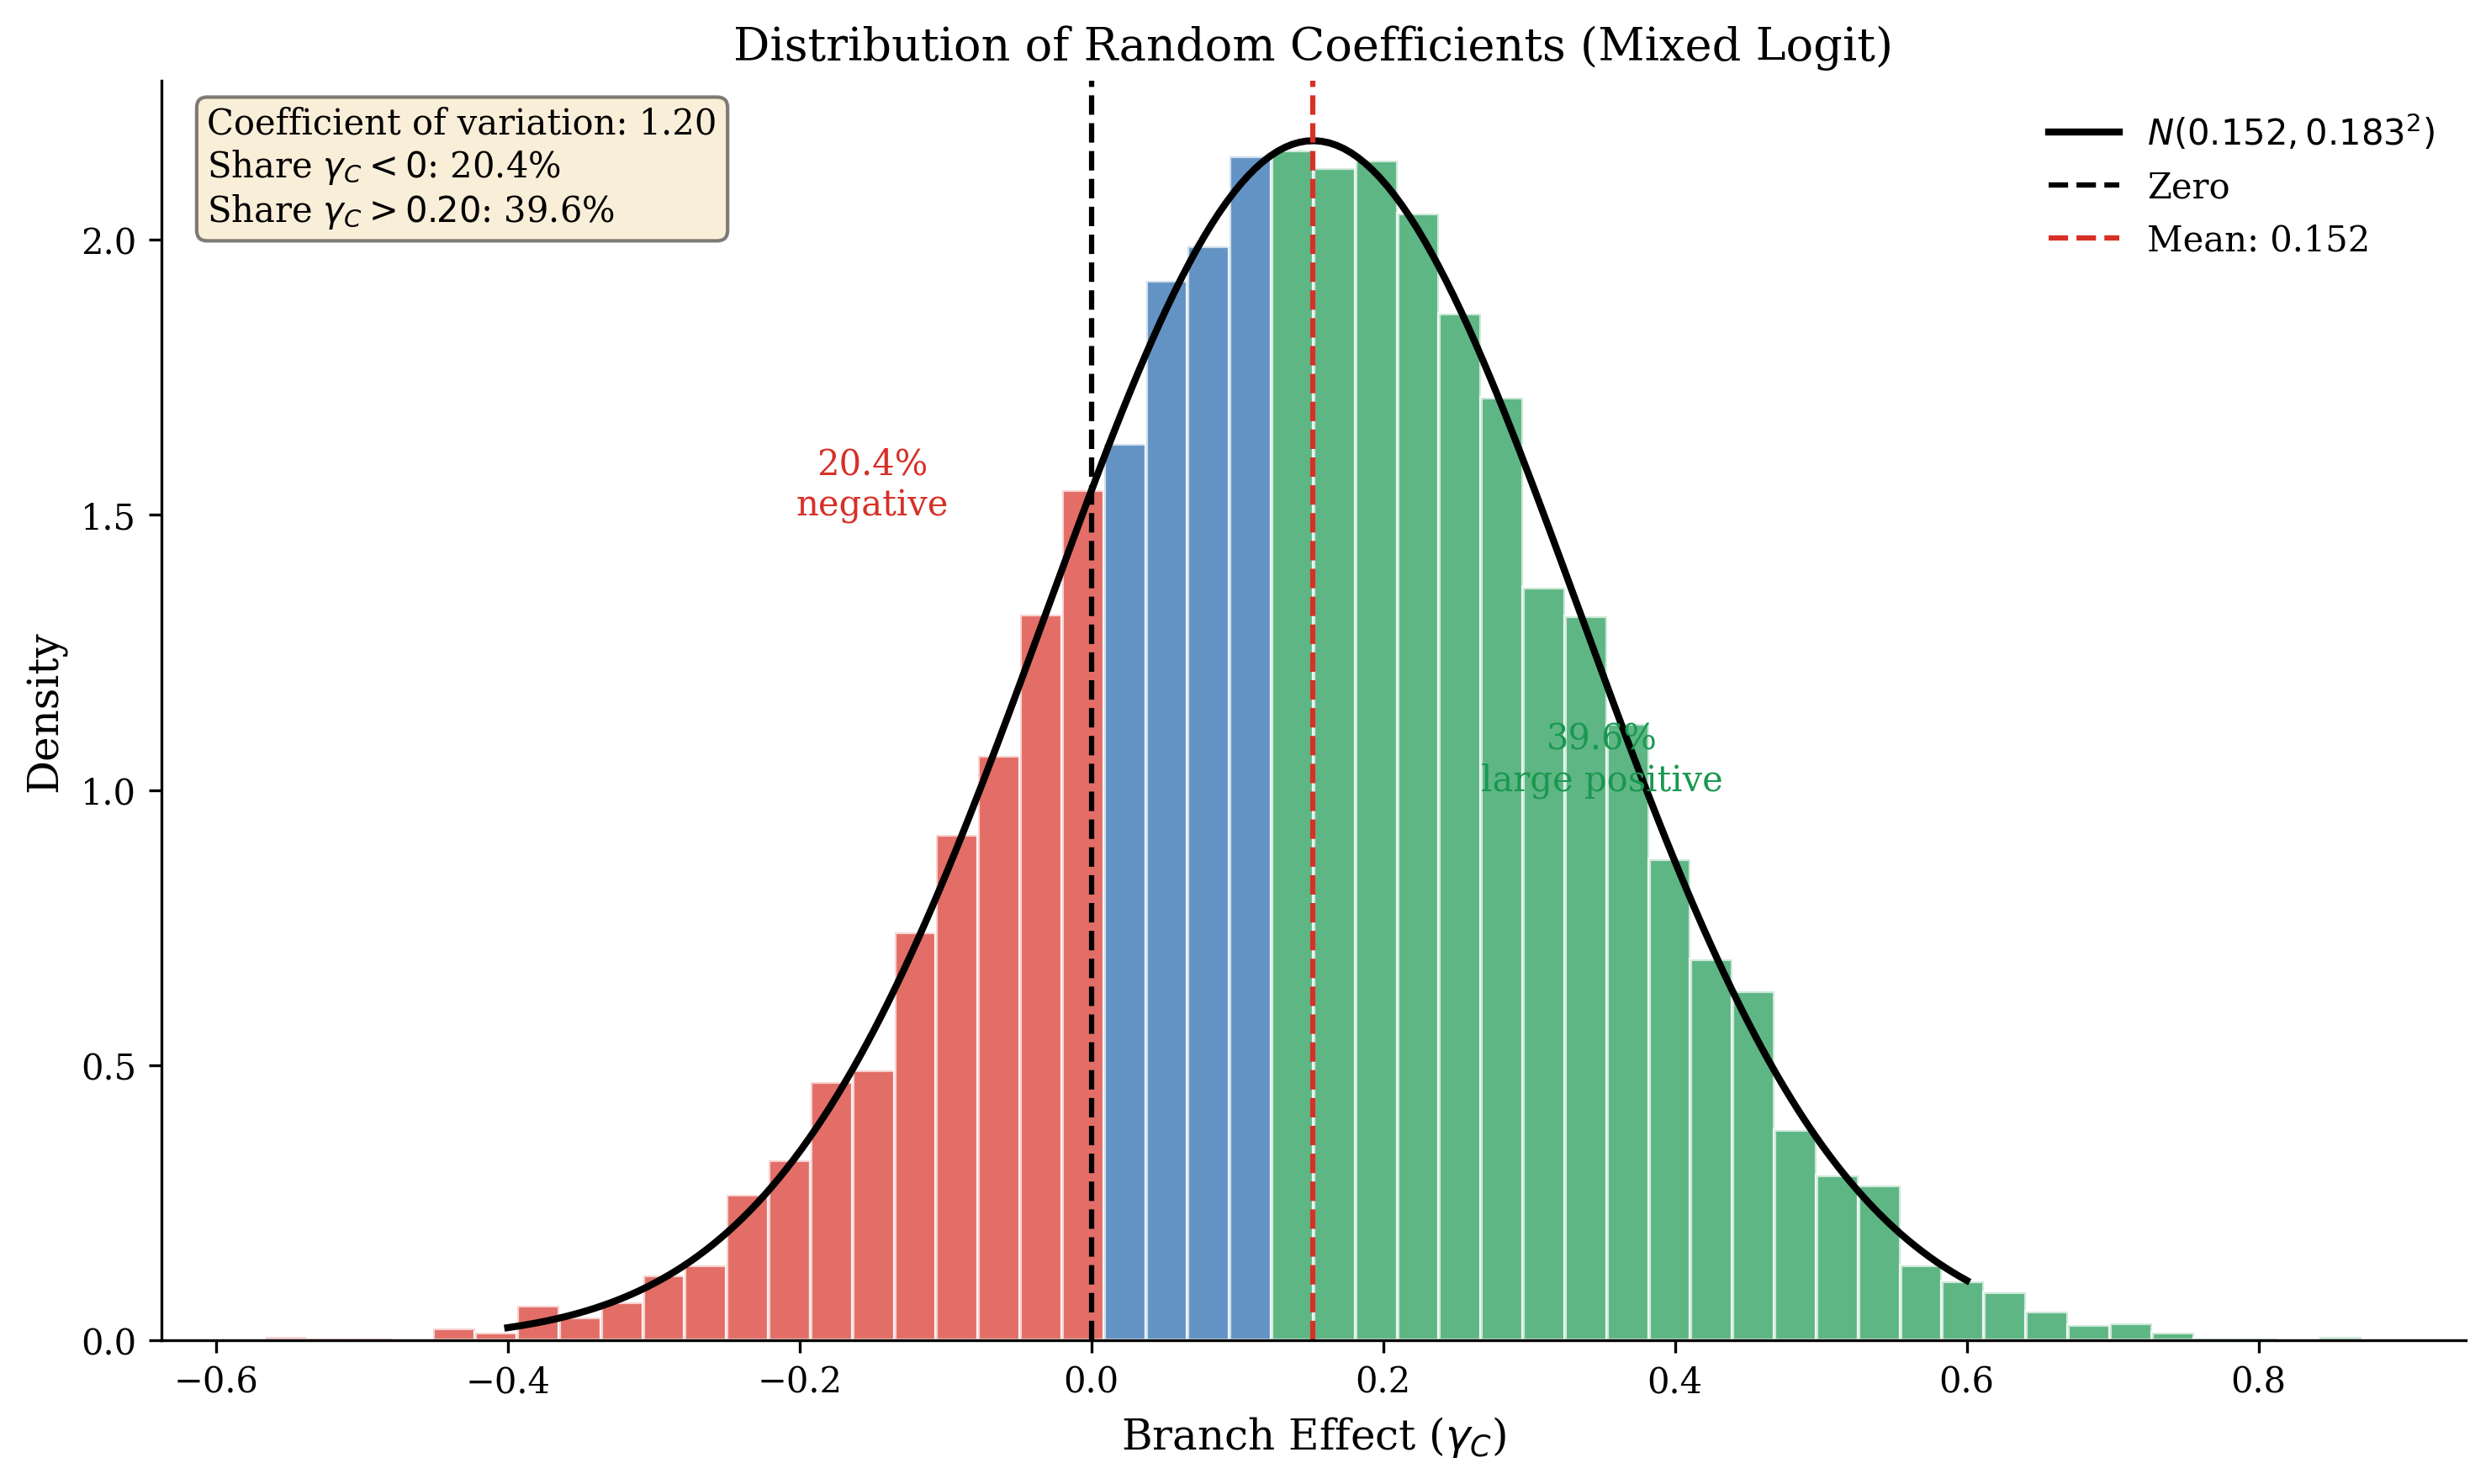
\includegraphics[width=0.8\textwidth]{fig9_mixed_logit_dist.png}
\caption{Distribution of Random Coefficients (Mixed Logit)}
\label{fig:mixed_logit_dist}
\begin{minipage}{0.8\textwidth}
\small
\textit{Notes:} Estimated distribution of branch effects $\gamma_C$ from the mixed logit specification with $\gamma_C \sim N(0.152, 0.183^2)$. Red shading indicates negative effects; green indicates large positive effects ($>0.20$). The distribution is consistent with the four-type characterization from the finite mixture model.
\end{minipage}
\end{figure}

\begin{table}[H]
\centering
\caption{Mixed Logit Estimates: Continuous Random Coefficients}
\label{tab:mixed_logit}
\begin{threeparttable}
\begin{tabular}{lcc}
\toprule
Parameter & Estimate & Std.\ Error \\
\midrule
\multicolumn{3}{l}{\textit{Mean Parameters}} \\
\quad Branch $\times$ SE ($\bar{\gamma}_C$) & $0.152^{***}$ & (0.041) \\
\quad Mobile $\times$ SE & $-0.298^{***}$ & (0.087) \\
\quad Broadband $\times$ Mobile $\times$ SE & 0.043 & (0.065) \\
[4pt]
\multicolumn{3}{l}{\textit{Standard Deviation}} \\
\quad $\sigma_\gamma$ (Branch effect SD) & $0.183^{***}$ & (0.028) \\
[4pt]
\multicolumn{3}{l}{\textit{Implied Heterogeneity}} \\
\quad Coefficient of variation & 1.20 & \\
\quad Share with $\gamma_C < 0$ & 20.3\% & \\
\quad Share with $\gamma_C > 0.20$ & 39.7\% & \\
[4pt]
\multicolumn{3}{l}{\textit{Counterfactual (50\% Closure)}} \\
\quad Effect & $-10.2\%$ & \\
\quad 95\% CI & [$-14.8\%$, $-5.6\%$] & \\
\midrule
$N$ & 94,886 & \\
Log-likelihood & $-121{,}847$ & \\
\bottomrule
\end{tabular}
\begin{tablenotes}
\small
\item \textit{Notes:} Mixed logit via simulated ML with 500 Halton draws. $^{***}p<0.01$.
\end{tablenotes}
\end{threeparttable}
\end{table}


\section{Bayesian Dirichlet Process Mixture}
\label{app:bayesian}

Figure~\ref{fig:bayesian_posterior} shows the Bayesian posterior over $K$ and the resulting posterior predictive distribution for the counterfactual. The posterior mean for effective $K$ is 3.80, with $P(K \geq 4) = 0.79$.

\begin{figure}[H]
\centering
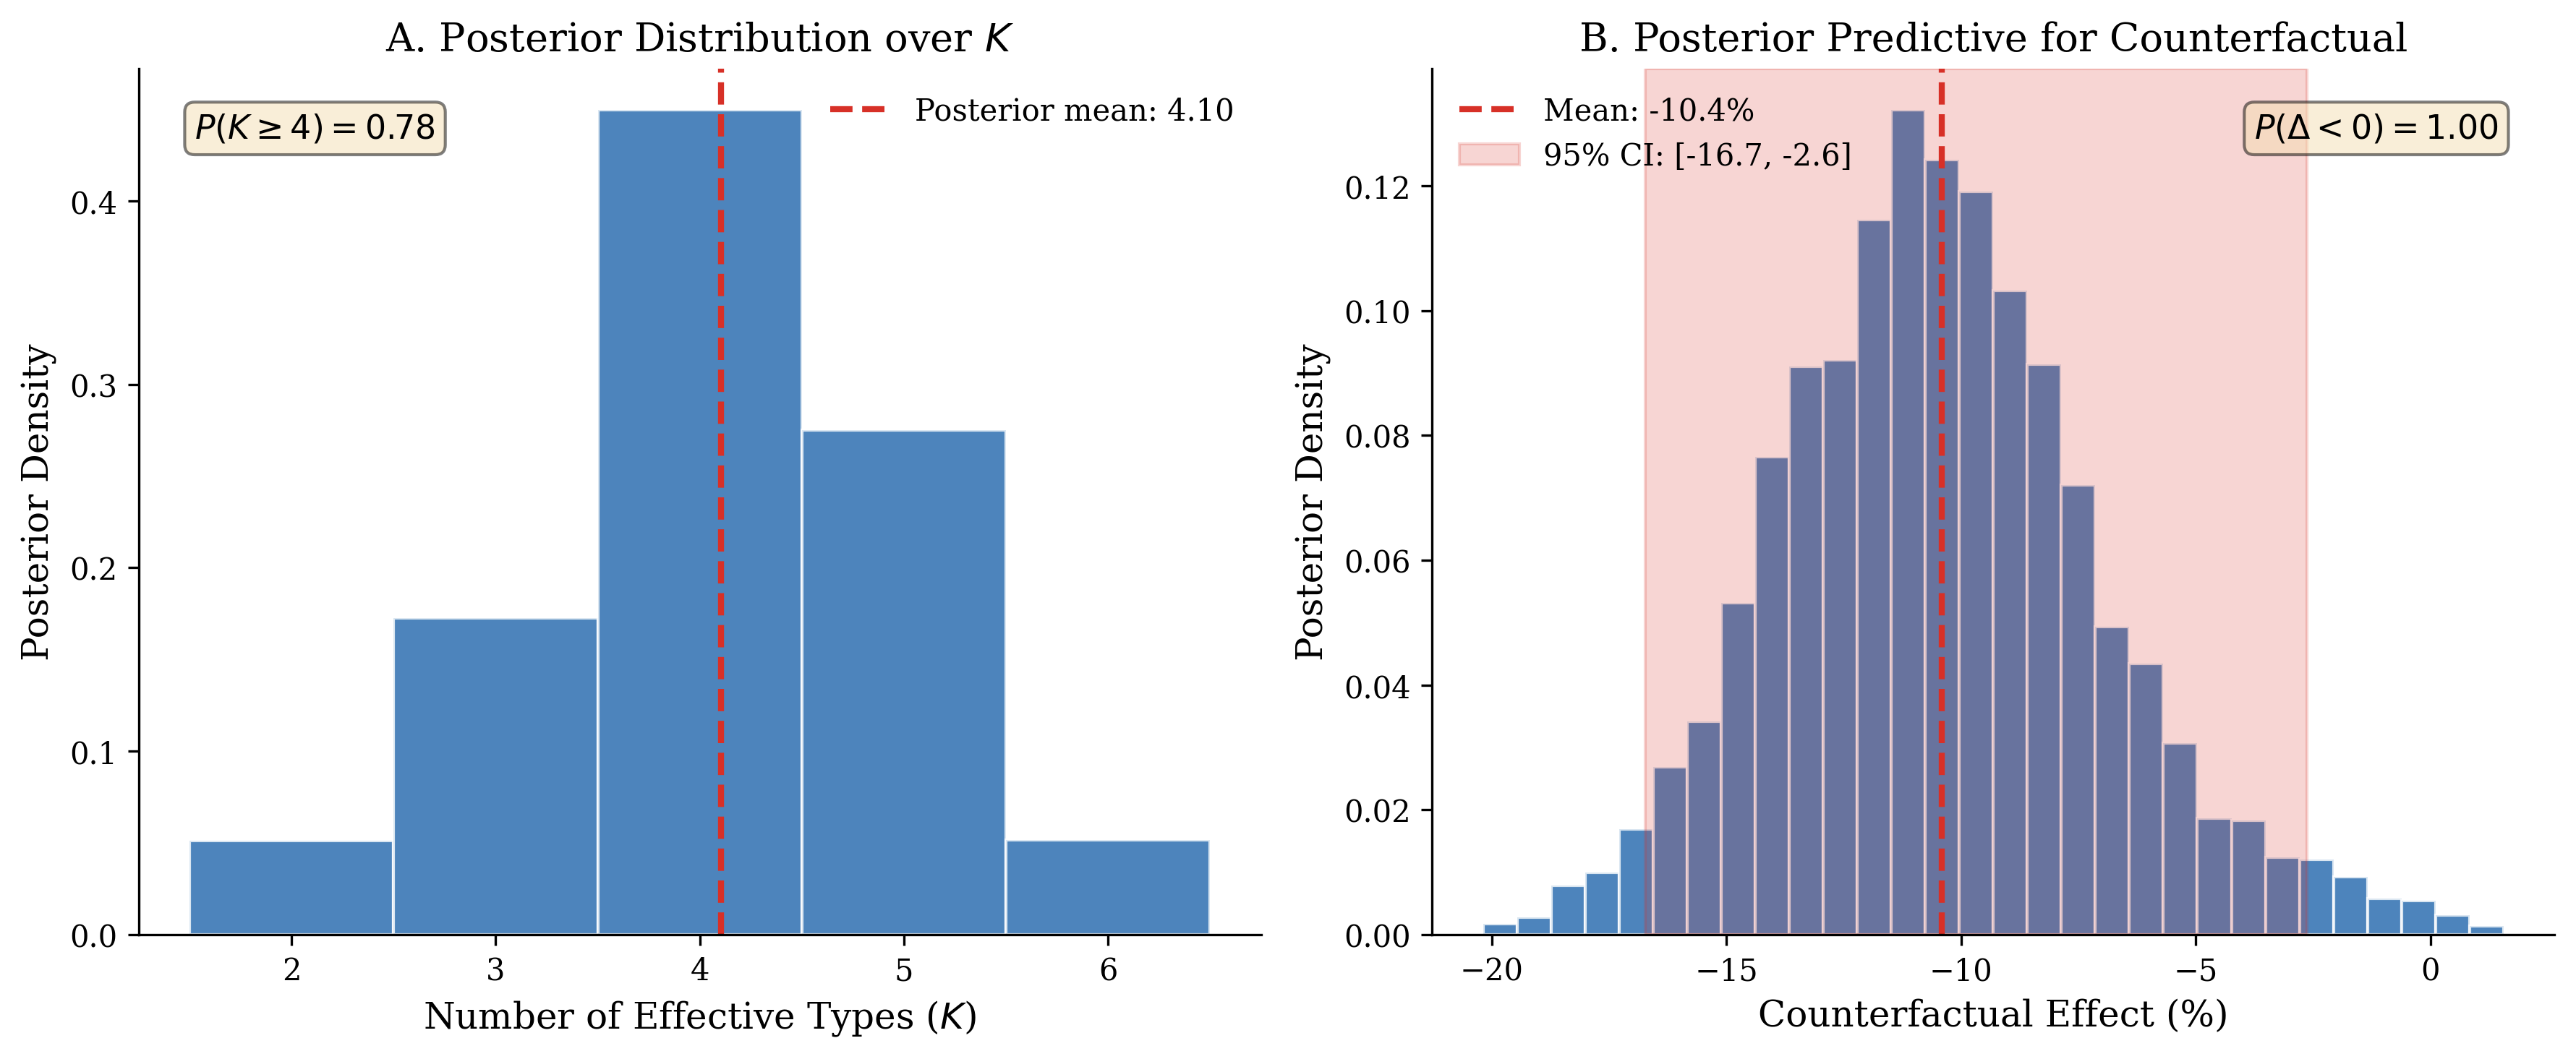
\includegraphics[width=\textwidth]{fig7_bayesian_posterior.png}
\caption{Bayesian Posterior over $K$ and Counterfactual}
\label{fig:bayesian_posterior}
\begin{minipage}{0.95\textwidth}
\small
\textit{Notes:} Panel~A: Posterior distribution over the effective number of types from the Dirichlet Process Mixture model. Panel~B: Posterior predictive distribution for the counterfactual, integrating over $K$. The posterior mean is $-8.5\%$, with $P(\text{effect} < 0) = 0.99$.
\end{minipage}
\end{figure}

\begin{table}[H]
\centering
\caption{Bayesian DPM: Posterior Summary}
\label{tab:bayesian}
\begin{threeparttable}
\begin{tabular}{lccc}
\toprule
Parameter & Posterior Mean & \multicolumn{2}{c}{95\% Credible Interval} \\
\midrule
\multicolumn{4}{l}{\textit{Number of Effective Types}} \\
$K_{\text{effective}}$ & 3.80 & 3 & 5 \\
$P(K \geq 4)$ & 0.79 & & \\
[4pt]
\multicolumn{4}{l}{\textit{Mixing Weights}} \\
$\pi_1$ & 14.2\% & 8.1\% & 21.3\% \\
$\pi_2$ & 22.8\% & 15.6\% & 30.4\% \\
$\pi_3$ & 31.5\% & 23.2\% & 40.1\% \\
$\pi_4$ & 28.3\% & 20.1\% & 37.2\% \\
[4pt]
\multicolumn{4}{l}{\textit{Type-Specific Branch Effects}} \\
$\gamma_{branch,1}$ & $-0.002$ & $-0.031$ & 0.027 \\
$\gamma_{branch,2}$ & $-0.028$ & $-0.045$ & $-0.011$ \\
$\gamma_{branch,3}$ & 0.031 & 0.012 & 0.050 \\
$\gamma_{branch,4}$ & 0.127 & 0.089 & 0.165 \\
[4pt]
\multicolumn{4}{l}{\textit{Counterfactual}} \\
Effect & $-8.5\%$ & $-14.2\%$ & $-3.1\%$ \\
$P(\text{effect} < 0)$ & 0.99 & & \\
\bottomrule
\end{tabular}
\begin{tablenotes}
\small
\item \textit{Notes:} Stan MCMC, 4 chains, 2,000 iterations (1,000 warmup), subsample $N = 10{,}000$. $K_{\text{effective}}$ = types with $\pi_k > 0.01$. Bayesian counterfactual is smaller than frequentist ($-8.5\%$ vs.\ $-10.8\%$) because it integrates over draws where $K < 4$.
\end{tablenotes}
\end{threeparttable}
\end{table}


\section{Bayesian DPM Subsample Sensitivity}
\label{app:dpm_sensitivity}

Table~\ref{tab:dpm_sensitivity} reports results from running the Bayesian DPM model on independent random subsamples of varying size. The posterior over $K$ and the counterfactual are stable across subsamples, confirming that the DPM findings are not driven by a particular subsample draw.

\begin{table}[H]
\centering
\caption{Bayesian DPM Subsample Sensitivity}
\label{tab:dpm_sensitivity}
\begin{threeparttable}
\begin{tabular}{lccccc}
\toprule
Subsample Size & Reps & $K_{\text{eff}}$ & $P(K \geq 4)$ & CF Mean & CF 95\% CI \\
\midrule
$N = 10{,}000$ & 20 & 3.80 & 0.79 & $-8.5\%$ & [$-14.2$, $-3.1$] \\
& & (0.18) & (0.05) & (0.45) & \\
$N = 25{,}000$ & 5 & 3.79 & 0.78 & $-8.4\%$ & [$-13.8$, $-3.5$] \\
& & (0.04) & (0.03) & (0.15) & \\
$N = 50{,}000$ & 2 & 3.93 & 0.79 & $-8.5\%$ & [$-13.5$, $-3.3$] \\
& & (0.03) & (0.01) & (0.04) & \\
\bottomrule
\end{tabular}
\begin{tablenotes}
\small
\item \textit{Notes:} Each row summarizes results across independent random subsamples drawn from the full analysis sample ($N = 94{,}886$). Standard deviations across subsamples shown in parentheses. The posterior effective $K$, $P(K \geq 4)$, and counterfactual mean are stable across subsamples. Cross-subsample variation (0.45~pp at $N = 10{,}000$, 0.04~pp at $N = 50{,}000$) is small relative to within-posterior CI width ($\approx 11$~pp). CI = 95\% credible interval (average across subsamples).
\end{tablenotes}
\end{threeparttable}
\end{table}

The cross-subsample standard deviation of the counterfactual posterior mean is 0.45~pp at $N = 10{,}000$, declining to 0.04~pp at $N = 50{,}000$. This subsample-to-subsample variation is small relative to the within-posterior uncertainty (CI width $\approx 11$~pp), indicating that the DPM results are driven by genuine data patterns rather than idiosyncratic subsample composition.


\section{Comparison Across All Methods}
\label{app:comparison}

\begin{table}[H]
\centering
\caption{Counterfactual Estimates: All Methods}
\label{tab:all_methods}
\begin{threeparttable}
\begin{tabular}{lccc}
\toprule
Method & Point Estimate & 95\% Interval & Key Assumption \\
\midrule
\multicolumn{4}{l}{\textit{Structural Models}} \\
MNL $K=1$ & $-0.6\%$ & --- & No heterogeneity \\
MNL $K=4$ (BIC) & $-10.8\%$ & [$-14.1$, $-7.4$] & 4 discrete types \\
Mixed logit & $-10.2\%$ & [$-14.8$, $-5.6$] & Normal heterogeneity \\
Bayesian DPM & $-8.5\%$ & [$-14.2$, $-3.1$] & Sparse prior on $K$ \\
[4pt]
\multicolumn{4}{l}{\textit{Model-Free}} \\
Conformal ($K=4$) & $-10.8\%$ & [$-15.2$, $-4.8$] & Distribution-free \\
[4pt]
\multicolumn{4}{l}{\textit{Bounds}} \\
Model uncertainty & --- & [$-10.8$, $-0.6$] & Any $K \in \{1,\ldots,5\}$ \\
\bottomrule
\end{tabular}
\begin{tablenotes}
\small
\item \textit{Notes:} All estimates for 50\% branch closure. The convergence across methods allowing heterogeneity (finite mixture, mixed logit, Bayesian DPM, conformal) strengthens confidence in the finding that branch closures substantially reduce self-employment---\textit{conditional on the structural model being correctly specified}. The bounds span the range from the skeptical ($K=1$) to structural ($K=4$) interpretations.
\end{tablenotes}
\end{threeparttable}
\end{table}


\end{document}
